% ===============================================
% ===============================================
% LaTeX Thesis Template
%
% Author: Julian Haase
% E-Mail: Julian.Haase@tu-dresden.de
% Date: 14.05.2018
% Please contact the author in case of questions.
% ===============================================
% ===============================================
%
%
% ===============================================
%	Include Header File --- all LaTeX definitions stand here
% ===============================================
% !TEX root = thesis.tex
% ===============================================
% ===============================================
% 	LaTeX Header File - Defines all used packages and options
% ===============================================
% ===============================================
%
%
% ===============================================
% A. DOCUMENT CLASS (options and packages to use)
% ===============================================
\RequirePackage[ngerman=ngerman-x-latest]{hyphsubst}	% better German hyphenation rules
\documentclass[
	paper		= a4,	% Use A4 paper
	english,
%	ngerman,
	BCOR=4mm,		% Additional border for binding the document
	scale=0.95,
	% BCOR depending on the number of pages
	% Bei 80g/m^2 Papier
	% 160 Seiten --> 8mm
	% 140 Seiten --> 7mm
	% 120 Seiten --> 6mm
	% ..
	% 60 Seiten --> 3mm
	% 40 Seiten --> 2mm
	% Bei 100g/m^2 Papier
	% 150 Seiten --> 9mm
	% 133 Seiten --> 8mm
	% 117 Seiten --> 7mm
	% 100 Seiten --> 6mm
	% 83 Seiten --> 5mm
	% 67 Seiten --> 4mm
	% 50 Seiten --> 3mm
	DIV=13,								% Proportion for empty and non-empty parts of a page
	%twoside,
	titlepage,							% Support for title environment
	headinclude		= true,				% Include header in typearea calculation
	footinclude		= false,			% Include footer in typearea calculation
	twoside			= false,			% Two-sided printing - true or false
	%cleardoublepage         = empty,	% Empty backsides for two-sided printing
	numbers 		= noenddot,			% Numbers (in headlines) without ending points
	parskip			= half,				% A half line to separate paragraphs
	chapterprefix	= false,			% Chapters with Prefix - true or false?
	appendixprefix	= false,			% Appendix with Prefix - true or false?
	headsepline,						% Line after header
	%headings 		= normal,			% Size of Headers (normal, small, big)
	bibliography	= totoc,			% Include Bibliography in Table of Contents
	listof 			= totoc,			% Include Lists in Table of Contents
	pagesize		= pdftex			% Define Typearea for pdftex usage
]{tudscrreprt} 			% load Koma-Script-Class for the CD of the TUD
\usepackage{scrhack}	% includes koma script patches for other packages
% ===============================================
%	Character coding and fonts for the document
% ===============================================
\usepackage[sfdefault]{noto}	% font for the CD
\usepackage[utf8]{inputenc}							% UTF-8 Support
\usepackage[T1]{fontenc}							% T1 Fonts for font encoding
%\usepackage[ngerman]{babel}							% German language with new orthography
\usepackage[english]{babel}						% English language	
\usepackage[babel]{microtype}						% better layout of the text
% ===============================================
%	Package for quotation marks
% ===============================================
%\usepackage[babel=false, style=swiss]{csquotes}		% Swiss style quotes
%\usepackage[babel=false, german=quotes]{csquotes}		% German style quotes
\usepackage[babel=false, english=american]{csquotes}	% American style quotes
%\usepackage[babel=false, german=quotes]{csquotes}		% German style quotes
% ===============================================
%	Packages for additional table features
% ===============================================
\usepackage{array}			% Additional commands for tables
\usepackage{tabularx}		% Automatic row wide with special parameter
\usepackage{booktabs}		% Packet for scientific table environments
\usepackage{longtable}		% Support for tables over multiple pages
\usepackage{multirow}		% Support for spanning cells over multiple rows
\usepackage{longtable}		% For tables longer than one site
\usepackage{ltxtable}		% use X column from tabularx in longtable
\usepackage{tabu}		% For the symbol table only
% ===============================================
%	Packages for additional mathemtical features
% ===============================================
\usepackage{amsmath, amsthm, amssymb}	% ASM Mathematic packages
\usepackage{pifont}						% used for circled numbers
\usepackage{siunitx}					% Numbers with nice untis
% ===============================================
%	Packages for figures and captions
% ===============================================
\usepackage{pdfpages}	% Einbinden von PDF als komplette Seite
\usepackage{graphicx}	% Einbinden von Bildern				
\usepackage{caption}	% Packet to support captions for subfigures
\usepackage{subcaption}	% Packet to support subfigure environments
%\renewcommand\thesubfigure{(\alph{subfigure})}% für Klammern bei Referenz der Subfigure(z. B. Abbildung 3.1(a))
% ===============================================
%	Additional packages
% ===============================================
\usepackage{isodate}			% for several date formats
\usepackage{xcolor}				% Packet for colour text support
\usepackage{enumitem}			% Alternitive Item environment for customizing lists
\usepackage{flafter}			% Never insert figures before the actual reference
\usepackage[section]{placeins}	% Insert floatbarriers before every section
\usepackage{ellipsis}			% Corrects wrong spaces after dots
\usepackage{blindtext}
%\usepackage{easy-todo}			% for colored Todo-Notes in the PDF
% ===============================================
%	Packages for references and citation
% ===============================================
\usepackage[%
	backend=biber,		% for sorting the entries and citing information with UTF-8 support
	style=numeric,	% style for citation
	url=false,			% url-field of the bib is not printet in the references
	maxalphanames=1,	% 
	maxcitenames=1,		%
	]%
{biblatex}	%
\addbibresource{bib/references.bib}	% Adding the bib-file to reference, if need more copy this command
% ===============================================
%	Packages for special PDF features and References
% ===============================================
\usepackage[%
	pdfauthor={Yike Jing},			%
	pdftitle={Thesis},		%
	pdfsubject={Master's Thesis},			%
	pdfkeywords={},						%
	pdfcreator={PdfLaTeX},				%
	pdfproducer	={LaTeX with hyperref},	%
	breaklinks=true,	%
	colorlinks=true,	%
	% 	PDF-options for PRINT OUT of the document			    
	%	urlcolor=black,     %
	%	citecolor=black,    %
	%	linkcolor=black,    %
	%	filecolor=black,	%
	% 	PDF-options for PDF file creation (e.g. coloured links)
	urlcolor=blue,      %
	citecolor=red,      %
	linkcolor=blue,     %
	filecolor=blue,		%		
	bookmarks,				%
	bookmarksopen,			%
	bookmarksopenlevel=1,	%
	bookmarksnumbered,		%	
	pdfpagelabels,			%
	pdfdisplaydoctitle, 	%
	pdfpagemode=UseOutlines,%
	linktoc=all, 			%
	]%
{hyperref}%
\usepackage[%
	open,			%
	openlevel=2, 	%
	]%
{bookmark}%
\usepackage[nameinlink,noabbrev]{cleveref} % simpler refs with \cref
% ===============================================
%	Packages for glossary (acronyms, symbols, etc.)
% ===============================================
\usepackage[%
	acronym,%
	symbols,%
	nomain,%
	nogroupskip,%
	toc,%
	section=chapter,%
	nostyles,%
	translate=babel,%
	%xindy={language=german-din},%
	%automake=immediate,
]{glossaries}
\makenoidxglossaries
%
%
% ===========================================================================
% B. SETTINGS (for the document and the packages)
% ===========================================================================
\pagestyle{headings}	% Headers with page title
\frenchspacing			% Limit the spacing after dots
\sisetup{locale = DE}	% german untis
%
%
% ===========================================================================
% C. NEW MAKROS AND ENVIRONMENTS (for later use in the document)
% ===========================================================================
%
% ===============================================
%	New Columtyps
% ===============================================
\newcolumntype{Y}{>{\centering\arraybackslash}X} % centered X columns for tablurarx
% ===============================================
%	\includegraphicstotab[..]{..}
% ===============================================
\newlength{\myx} % Saving the width of the figure
\newlength{\myy} % Saving the height of the figure
\newcommand\includegraphicstotab[2][\relax]{%
	% save the figure values
	\settowidth{\myx}{\includegraphics[{#1}]{#2}}%
	\settoheight{\myy}{\includegraphics[{#1}]{#2}}%
	% insert into to the cell of the table
	\parbox[c][1.1\myy][c]{\myx}{%
		\includegraphics[{#1}]{#2}}%
}%
% ===============================================
%	New Citation-Style [FirstAuthor Year]
% ===============================================
\renewcommand*{\labelalphaothers}{} %
\DeclareLabelalphaTemplate{%
	\labelelement{%
		\field[final]{shorthand}%
		\field{labelname}%
		\field{label}%
	}
	\labelelement{%
		\literal{\addhighpenspace}%
	}
	\labelelement{%
		\field{year}%
	}
}
% ===============================================
%	\newsymbol{label}{description}{symbol}{unit}
% ===============================================
\renewcommand*{\newsymbol}[5][]{%
	\newglossaryentry{#2}{%
		type=symbols,%
		name={#3},%
		description={\nopostdesc},%
		symbol={\ensuremath{#4}},%
		user1={\ensuremath{\mathrm{#5}}},%
		sort={#2},%
		#1%
	}%
}
\defglsentryfmt[symbols]{%
	\ifmmode%
	\glssymbol{\glslabel}%
	\else%
	\glsgenentryfmt~\glsentrysymbol{\glslabel}%
	\fi%
}
% ===============================================
%	Symbol table style for the glossary
% ===============================================
\newglossarystyle{symblongtabu}{%
	\renewenvironment{theglossary}{%
		\begin{longtabu}spread 0pt[l]{ccX<{\strut}l}%
		}{%
		\end{longtabu}%title
	}%
	\renewcommand*{\glsgroupheading}[1]{}%
	\renewcommand*{\glsgroupskip}{}%
	\renewcommand*{\glossaryheader}{%
		\toprule
		\bfseries Formelzeichen & \bfseries Einheit &
		\bfseries Bezeichnung & \bfseries Seite(n)
		\tabularnewline\midrule\endhead%
		\bottomrule\endfoot%
	}%
	\renewcommand*{\glossentry}[2]{%
		\glsentryitem{##1}% Entry number if required
		\glstarget{##1}{\glossentrysymbol{##1}} &
		\glsentryuseri{##1} &
		\glossentryname{##1} &
		##2\tabularnewline%
	}%
}
% ===============================================
%	Acronym table style for the glossary
% ===============================================
\newglossarystyle{acrotabularx}{%
    \renewenvironment{theglossary}{%
        \begin{longtable}{@{}%
            p{0.15\textwidth}%
            p{0.53\textwidth}%
            p{0.24\textwidth}%
        @{}}
    }{%
        \end{longtable}%
    }%
    \renewcommand*{\glossaryheader}{}%
    \renewcommand*{\glsgroupheading}[1]{}%
    \renewcommand*{\glsgroupskip}{}%
    \renewcommand*{\glossentry}[2]{%
        \glstarget{##1}{%
            \sffamily\bfseries\glossentryname{##1}%
        } &
        \glossentrydesc{##1} &
        \raggedright ##2\tabularnewline
    }%
}
% ===============================================
%	Macros for fixme entries etc.
% ===============================================
% Macro for fixme entries
\newcommand{\fixme}[1]{\textcolor{blue}{FIXME: #1}}
% Macro for change entries
\newcommand{\change}[1]{\textcolor{green}{CHANGE: #1}} 
% Macro for remark entries
\newcommand{\remarks}[1]{\textcolor{magenta}{REMARKS: #1}} 
\newcommand{\re}{\textcolor{cyan}{\textbf{[ref]}}} 
% A Makro to support rephrase suggestions
% use as follows: rephrase{original}{new(suggestion)}{reason}, for no reason leave last argument empty!
\definecolor{darkgreen}{rgb}{0.0,0.6,0.0}
\newcommand{\rephrase}[3]{\textcolor{red}{#1}\footnote{REPHRASE: #3} \textcolor{darkgreen}{#2}}
% ===============================================
%	Placeholder for figures
% ===============================================
\newcommand{\missingfigure}[2][]{%
	\par
	\noindent
	\begin{tikzpicture}
	\draw[fill=black!40, draw = white, line width=0pt](-2, -2.5) rectangle +(\columnwidth, 4cm);
	\draw (2, -0.3) node[right, text width=\columnwidth-4.5cm] {#2};
	\draw[red, fill=white, rounded corners = 5pt, line width=10pt](30:2cm) -- (150:2cm) -- (270:2cm) -- cycle;
	\draw (0, 0.3) node {Missing};
	\draw (0, -0.3) node {Figure};
	\end{tikzpicture}
}% Ending \missingfigure command
%
%
% ===========================================================================
% D. ACTIONS AND OPERATIONS
% ===========================================================================
%
% ===========================================================================
% EOF
% ===========================================================================

% ===============================================
%	Symbols and acronyms for the glossaries package
% ===============================================
%\input{symbols}
% !TEX root = thesis.tex
% ===============================================
% ===============================================
% 	Acronyms
% ===============================================
% ===============================================
\newacronym{ai}{AI}{Artificial Intelligence}
\newacronym{ann}{ANN}{Artificial Neural Network}
\newacronym{asic}{ASIC}{Application-Specific Integrated Circuit}
\newacronym{bram}{BRAM}{Block Random-Access Memory}
\newacronym{cmos}{CMOS}{Complementary Metal-Oxide-Semiconductor}
\newacronym{cpu}{CPU}{Central Processing Unit}
\newacronym{ddr}{DDR}{Double Data Rate}
\newacronym{sdram}{SDRAM}{Synchronous Dynamic Random-Access Memory}
\newacronym{dfx}{DFX}{Dynamic Function Exchange}
\newacronym{dma}{DMA}{Direct Memory Access}
\newacronym{dpr}{DPR}{Dynamic Partial Reconfiguration}
\newacronym{dsp}{DSP}{Digital Signal Processing}
\newacronym{ff}{FF}{Flip-Flop}
\newacronym{fpga}{FPGA}{Field-Programmable Gate Array}
\newacronym{gpu}{GPU}{Graphics Processing Unit}
\newacronym{hdl}{HDL}{Hardware Description Language}
\newacronym{icap}{ICAP}{Internal Configuration Access Port}
\newacronym{if}{IF}{Integrate-and-Fire}
\newacronym{iot}{IoT}{Internet of Things}
\newacronym{ip}{IP}{Intellectual Property}
\newacronym{lif}{LIF}{Leaky Integrate-and-Fire}
\newacronym{lut}{LUT}{Lookup Table}
\newacronym{pcap}{PCAP}{Processor Configuration Access Port}
\newacronym{pl}{PL}{Programmable Logic}
\newacronym{ps}{PS}{Processing System}
\newacronym{ram}{RAM}{Random-Access Memory}
\newacronym{rm}{RM}{Reconfigurable Module}
\newacronym{rom}{ROM}{Read-Only Memory}
\newacronym{rp}{RP}{Reconfigurable Partition}
\newacronym{rtl}{RTL}{Register-Transfer Level}
\newacronym{sdsp}{SDSP}{Spike-Driven Synaptic Plasticity}
\newacronym{snn}{SNN}{Spiking Neural Network}
\newacronym{soc}{SoC}{System-on-Chip}
\newacronym{stdp}{STDP}{Spike-Timing-Dependent Plasticity}
%\newacronym{label}{acronym}{description}


\begin{document}
% ===============================================
%	Title Page
% ===============================================
\pagenumbering{Alph} % Alphanumeric (capital) numbering for the PDF starting with A
% !TEX root = thesis.tex
% ===============================================
%	Heading for the chair
% ===============================================
%\faculty{Fakultät Informatik}
\faculty{Faculty of Computer Science}
%\institute{Institut für Technische Informatik}
\institute{Institute of Computer Engineering}
%\chair{Professur für Adaptive Dynamische Systeme}
\chair{Chair of Adaptive Dynamic Systems}
\headlogo{logo/ADS_Logo.png}
\title{%
	FPGA-based Real-Time Learning Architecture with Partial
	Reconfiguration for Spiking Neural Networks
}
\subject{master} % or \thesis diploma, bachelor, student -> for details take a look at table 2.1 in tudscr.pdf
\title{%
  FPGA-based Real-Time Learning Architecture with Partial Reconfiguration for Spiking Neural Networks
}
\graduation[M.Sc.]{Master of Science}
\author{
	Yike Jing
	\matriculationnumber{5201619}%
	\dateofbirth{3.9.2000}%
	\placeofbirth{Zhejiang}%
	\matriculationyear{2023}%
	\course{Nanoelectronic Systems}
}
\supervisor{Gloria Sepanta \and Dr.-Ing. Lester Kalms}
\professor{Prof. Dr. Diana Göhringer \and Prof. Dr. rer. nat. Josef Weidendorfer \and Prof. Dr. Ir. Nele Mentens}
\date{\today}
%\makecover
\maketitle
	
% ===============================================
%	Task
% ===============================================
\IfFileExists{../TaskDescription.pdf}{
  \includepdf[pages=-]{../TaskDescription.pdf}  % Use the created Artifact in CI/CD environment; This will either be the compiled version in the TaskDescription directory or the printed version of the TaskDescriptionSigned.pdf
}{
  \IfFileExists{TaskDescriptionSigned.pdf}
  {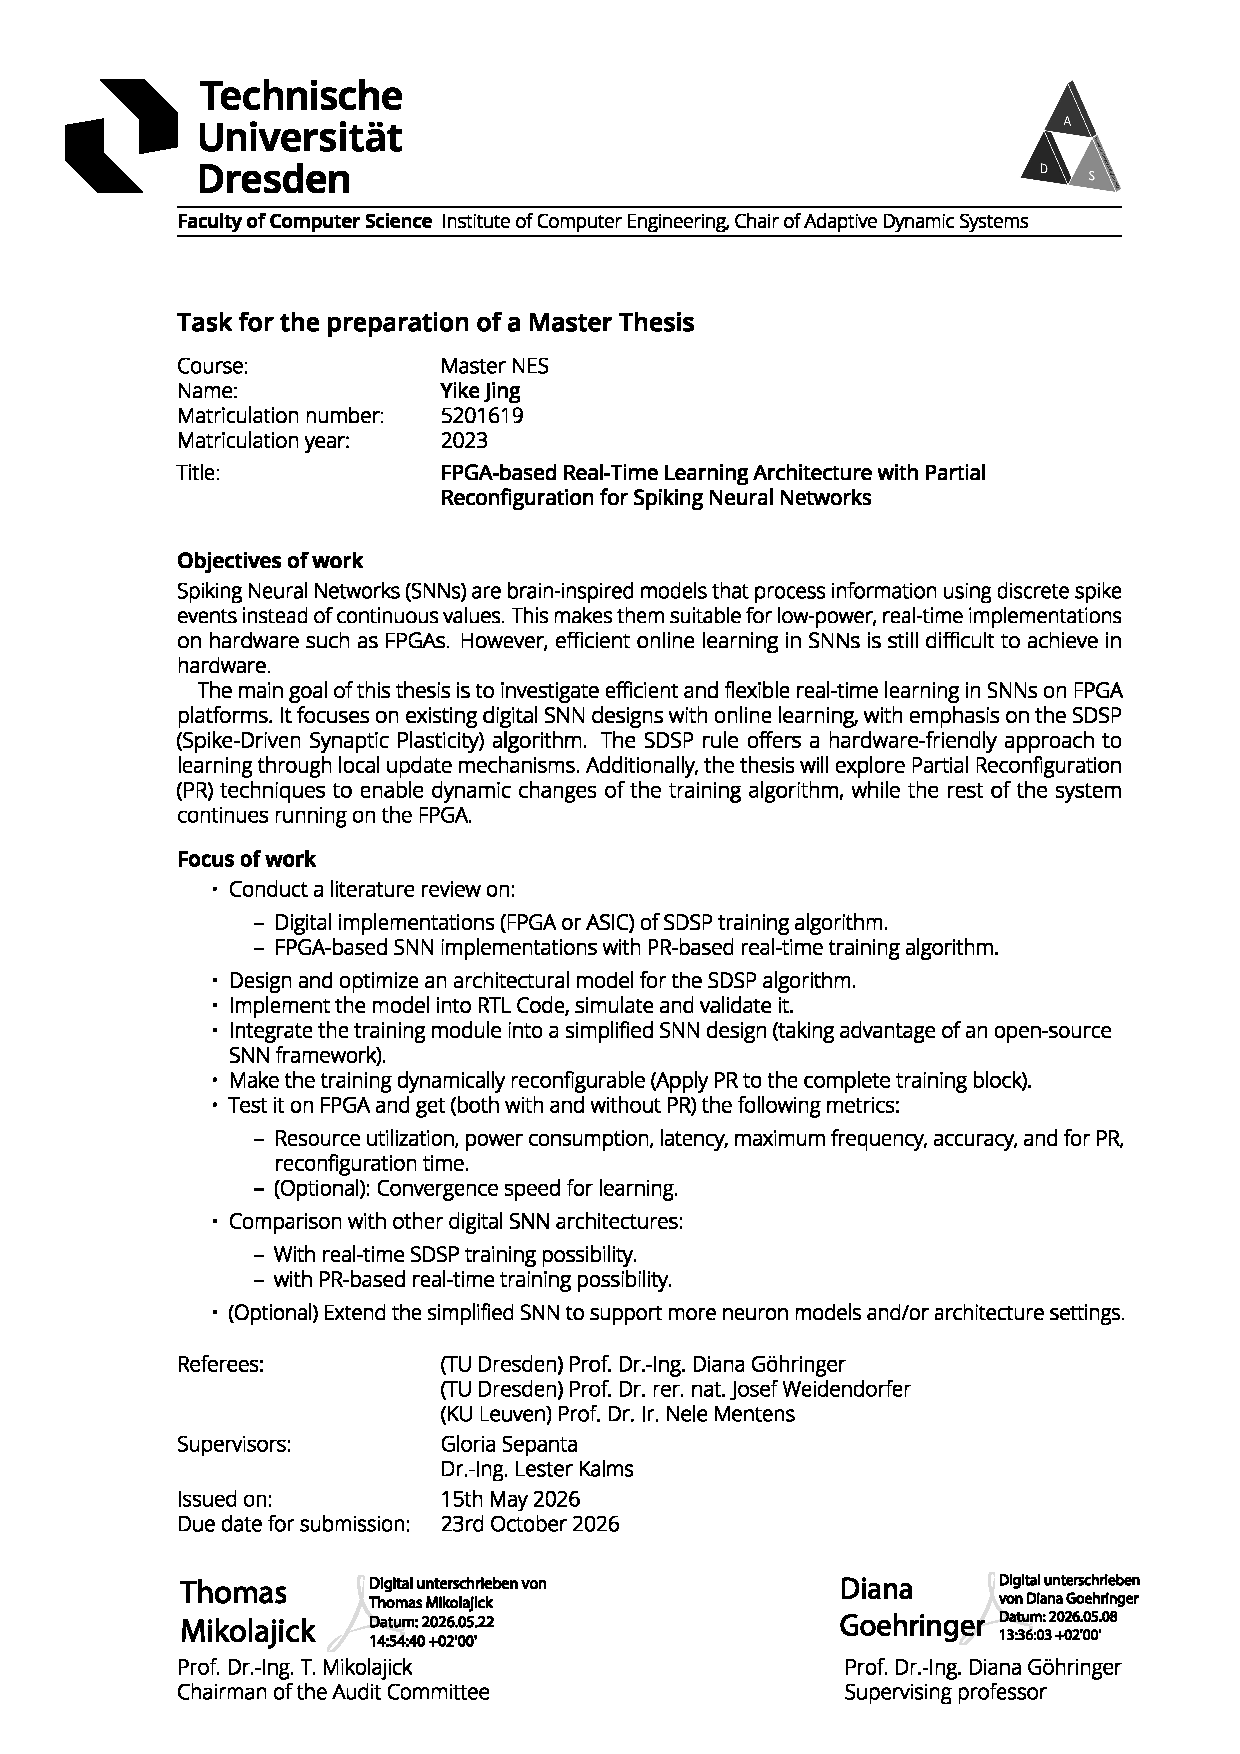
\includepdf[pages=-]{TaskDescriptionSigned.pdf}}   % Use the signed (non-printed) version of the task description second, else the compiled or the fallback.
  {
\includepdf[pages=-]{TaskDescription.pdf}}         % Use local file in normal LaTeX environment if artifact is not available
}
\bookmark[page=2]{Aufgabenstellung}
% ===============================================
%	Confirmation
% ===============================================
% Comment this line if Statementofauthorship.pdf exist
\confirmationclosing{%
  \medskip\noindent Dresden,\nobreakspace\today\\[8ex]%
  \begin{minipage}{5cm}%
    Yike Jing\\[0.5ex]%
    
\includegraphics[width=4.4cm]{figures/signature.jpg}%
  \end{minipage}%
}
\confirmation[supporter=Gloria Sepanta \and Dr.-Ing. Lester Kalms,pagestyle=empty.tudheadings]

\IfFileExists{./Statementofauthorship.pdf}
  {\includepdf[pages=-]{./Statementofauthorship.pdf}} 
\bookmark[page=3]{Selbstständigkeitserklärung}
% ===============================================
%	Abstract
% ===============================================	
% !TEX root = thesis.tex
% ===============================================
% ===============================================
%	Abstract in german and english
% ===============================================
% ===============================================
\TUDoption{abstract}{multiple,section,notoc}
\renewcaptionname{english}{\abstractname}{Abstract}
\begin{abstract}[pagestyle=empty.tudheadings]%
Spiking Neural Networks (SNNs) offer a promising approach to energy-efficient and low-latency edge intelligence by processing information through discrete spike events. Field-Programmable Gate Arrays (FPGAs) are well suited to this model because they provide configurable parallelism and deterministic execution. However, most FPGA-based SNN accelerators use fixed synaptic weights, whereas online learning additionally requires neuron state, writable weight storage, and coordinated memory access. Previous neuromorphic processors demonstrate local learning but often rely on fixed, task-specific architectures, leaving a gap between specialized systems and reusable FPGA-generation frameworks.

This thesis addresses that gap by extending an accelerator generated by the open-source Spiker+ framework with a synthesizable Spike-Driven Synaptic Plasticity (SDSP) learning path. The Spiker+ hierarchy is retained while the postsynaptic states required by SDSP are exposed. The architecture combines local state evaluation, bounded updates, writable excitatory-weight memory, and an address-aligned read--modify--write mechanism that preserves the association between updated weights and their original addresses. Learning is selectable at runtime, and the same hardware retains an inference-only mode without issuing new weight writes.

The modified SNN and its learning and communication modules are packaged as a reusable Vivado IP core and deployed on a PYNQ-Z1. AXI4-Lite and AXI DMA connect the accelerator to a PYNQ runtime that prepares inputs, configures operation, transfers spike data, and retrieves classification results. Self-checking simulations, interface tests, and board-level experiments confirm correct supervision, persistent weight-dependent behaviour, and continuous operation across complete training epochs.

The implemented system meets timing at 100~MHz on the XC7Z020 and uses 5,056 lookup tables, 5,294 flip-flops, and four block RAMs. Including processor and transfer overhead, the complete application achieves approximately 66--68 images per second. In one continuous experiment, the accelerator completed 180,000 supervised transactions over three MNIST epochs. Strict accuracy on a fixed 1,000-image validation set increased from 5.9\% to 39.6\%. The single-layer 784--10 network provides a structural reference to TEDOP, while differences in models, precision, and measurement boundaries prevent a direct performance ranking. Overall, the results demonstrate persistent online adaptation and successful system-level integration into the reusable Spiker+ flow. They establish hardware feasibility, but not learning convergence, because only one parameter configuration and three epochs were evaluated. Longer training, parameter exploration, increased network capacity, and reduced processor-side overhead remain future work.
\end{abstract}

\bookmark[page=4]{Kurzfassung/Abstract}

\pagenumbering{Roman} % Roman numbering for the PDF starting with I
% ===============================================
%	Table of contents
% ===============================================
\tableofcontents
\clearpage
% ===============================================
%	Table of figures
% ===============================================
\listoffigures
\clearpage
% ===============================================
%	Table of tables
% ===============================================
\listoftables
\clearpage
% ===============================================
%	Table of listings
% ===============================================
%
% ===============================================
%	Table of acronyms
% ===============================================
\printnoidxglossary[style=acrotabularx,title={Acronyms}]
  \clearpage

\pagenumbering{arabic} % arabic numbering for the PDF starting with 1
% ===============================================
%	Start of mainmatter - chapter 1 and so on...
% ===============================================
%\include{chapters/examples}%
% !TEX root = thesis.tex
\chapter{Introduction}
\label{sec:introduction}

The rapid development of \gls{ai} has led to its increasing use in areas such as autonomous systems, robotics, healthcare, and \gls{iot} devices. Many of these applications require data to be processed directly at the edge, where decisions must be made with low latency and limited communication with cloud servers. However, traditional \gls{ai} models often require considerable computational resources, memory bandwidth, and energy, which makes their deployment on resource-constrained embedded devices challenging. These limitations have increased the demand for specialized hardware architectures that can provide efficient \gls{ai} processing while supporting real-time operation and adaptation to changing environments.

\section{Motivation and Problem Statement}
\label{subsec:motivation-and-problem-statement}

\Glspl{snn} are brain-inspired neural networks in which information is represented and communicated through discrete spike events. In contrast to conventional \glspl{ann}, their temporal state and binary event communication allow specialized hardware to exploit sparse activity and avoid some unnecessary computation and data movement. This processing model is attractive for low-latency and resource-constrained edge systems, provided that the hardware architecture preserves the event-driven characteristics of the network \cite{Carpegna2025}.

\Glspl{fpga} provide a suitable platform for exploring such architectures because they offer configurable parallelism, deterministic execution, and direct control over data flow, numerical representation, and memory organization. Neural operations can therefore be mapped to application-specific datapaths while the implementation remains modifiable during development. Spiker+ follows this approach by generating configurable VHDL accelerators for \gls{snn} inference from a high-level network description \cite{Carpegna2025}.

Many \gls{fpga}-based \gls{snn} accelerators, including the baseline Spiker+ flow considered in this work, focus on inference using parameters obtained through offline training. Their synaptic weights are initialized when the hardware is generated and remain fixed during normal execution. This approach separates training from deployment, but it prevents the implemented network from adapting its synaptic state directly on the target device. Adding online learning is not only a matter of implementing a learning equation: the required neuron state must be available at the correct time, the weight memory must support runtime writes, and every update must remain synchronized with the synaptic address being processed.

\Gls{sdsp} is well suited to this problem because a synaptic update is triggered by a presynaptic event and depends on information available locally at the synapse and postsynaptic neuron, including the membrane potential and a calcium-related estimate of recent firing activity \cite{Brader2007}. It avoids a global error-propagation datapath, but its integration still requires coordinated access to neuron state, bounded digital weights, and writable synaptic storage. The central problem addressed by this thesis is therefore how to introduce persistent \gls{sdsp}-based weight adaptation into the generated Spiker+ hierarchy without replacing its established inference schedule and neuron organization.

\section{Objective and Contributions}
\label{subsec:objective-and-contributions}

The objective of this thesis is to design, implement, and evaluate an \gls{fpga}-based \gls{snn} accelerator that supports \gls{sdsp} weight updates during network operation. The open-source Spiker+ framework is used as the inference baseline \cite{Carpegna2025}. The architecture generated by Spiker+ is extended while preserving its multi-cycle control, neuron datapaths, and recurrent output competition. When learning is enabled, the modified accelerator updates selected synaptic weights and retains them for subsequent input events. When learning is disabled, the same hardware remains available for inference without issuing new weight writes.

The implemented system also includes the hardware and software interfaces required for board-level operation. The complete accelerator is packaged as a Vivado \gls{ip} core and connected to the Zynq processing system through AXI4-Lite control, an AXI DMA input path, and an interrupt interface. A PYNQ runtime prepares the spike representation, configures inference or supervised learning, transfers complete samples from DDR, and retrieves the output spike counts and classification result. This system boundary allows the learning architecture to be evaluated on the PYNQ-Z1 rather than only through RTL simulation.

The main contributions of this thesis are:

\begin{itemize}
    \item a synthesizable digital \gls{sdsp} datapath that combines membrane-potential and calcium conditions with bounded, finite-width weight updates;
    \item the integration of ten local learning lanes, writable excitatory memory, and an address-aligned read--modify--write path into the generated Spiker+ layer while retaining an inference-only operating mode;
    \item the packaging and deployment of the complete accelerator in a PYNQ-Z1 system with processor control, DDR-to-stream data movement, runtime learning configuration, and observable transaction results; and
    \item multilevel verification and hardware evaluation demonstrating persistent teacher-guided weight adaptation, timing closure at 100~MHz, continuous execution of 180,000 training transactions, and an increase in strict MNIST validation accuracy from 5.9\% to 39.6\% over three epochs.
\end{itemize}

The reported accuracy is an intermediate result rather than a converged performance claim. The training experiment uses a single-layer network, one parameter configuration, and three epochs; the results were still changing at the final checkpoint. The evaluation therefore supports the functionality and integration of the online-learning architecture more strongly than it supports the classification performance of the selected configuration.

\Gls{dpr} was considered during the design process but was not implemented in the final system. The \gls{sdsp} module depends on algorithm-specific neuron state, memory organization, and update timing, and neither a second interface-compatible learning module nor a runtime-switching use case was available. A dedicated reconfigurable partition would consequently add implementation and verification complexity without providing useful functionality for the evaluated system. Chapter \ref{sec:design_methodology} documents this applicability assessment and the resulting scope decision.

\section{Thesis Organization}
\label{subsec:thesis-organization}

The remainder of this thesis is organized as follows. Chapter \ref{sec:background} introduces \glspl{snn}, the \gls{lif} neuron model, \gls{sdsp}, \gls{fpga}-based acceleration, the concepts required for the \gls{dpr} assessment, and the Spiker+ framework. Chapter \ref{sec:related_work} reviews digital online-learning processors and positions the proposed Spiker+ extension relative to existing \gls{sdsp}- and \gls{stdp}-based systems. Chapter \ref{sec:design_methodology} derives the online-learning architecture, describes the digital weight-update path and its integration into Spiker+, and assesses the applicability of \gls{dpr}. Chapter \ref{sec:implementation} presents the final RTL hierarchy, the packaged accelerator IP, the Vivado block design, the PYNQ runtime, and the verification infrastructure. Chapter \ref{sec:results_and_evaluation} reports the functional, implementation, runtime, and three-epoch learning results and compares them with TEDOP. Finally, Chapter \ref{sec:conclusion_and_future_work} summarizes the findings and identifies directions for improving training, encoding, network structure, and measurement.

% !TEX root = thesis.tex
\chapter{Background}
\label{sec:background}

This chapter introduces the theoretical and technical background required for the design and implementation presented in this thesis. It first describes the fundamental principles of Spiking Neural Networks and the Leaky Integrate-and-Fire neuron model. It then reviews the main learning approaches for \gls{snn}s and introduces the Spike-Driven Synaptic Plasticity rule in detail. The final sections present the concepts of \gls{fpga}-based neural-network acceleration and Dynamic Partial Reconfiguration required for the later design assessment, followed by the Spiker+ framework on which the implemented accelerator is based.

\section{Spiking Neural Networks}
\label{subsec: spiking neural networks}

\gls{snn}s are a class of biologically inspired neural networks that process and transmit information through discrete events known as spikes \cite{Maass1997,Gerstner2014}. They are commonly described as the third generation of \gls{ann}s. In traditional \gls{ann}s, neurons generally receive continuous-valued inputs, calculate a weighted sum, and apply an activation function to produce a continuous-valued output \cite{Maass1997}. In contrast, a spiking neuron maintains an internal state that evolves over time and generates an output spike only when a firing condition is satisfied. Therefore, \gls{snn}s introduce an explicit temporal dimension into neural information processing.

An \gls{snn} generally consists of interconnected spiking neurons and synapses \cite{Gerstner2014}. Each synapse connects a presynaptic neuron to a postsynaptic neuron and is associated with a synaptic weight. When a presynaptic spike arrives, it changes the internal state of the postsynaptic neuron according to the corresponding weight. Excitatory synapses increase the likelihood that the postsynaptic neuron will fire, whereas inhibitory synapses reduce it. The neuron integrates these synaptic events over time and produces an output spike when its membrane potential reaches a defined threshold.

\begin{figure}[t]
	\centering
	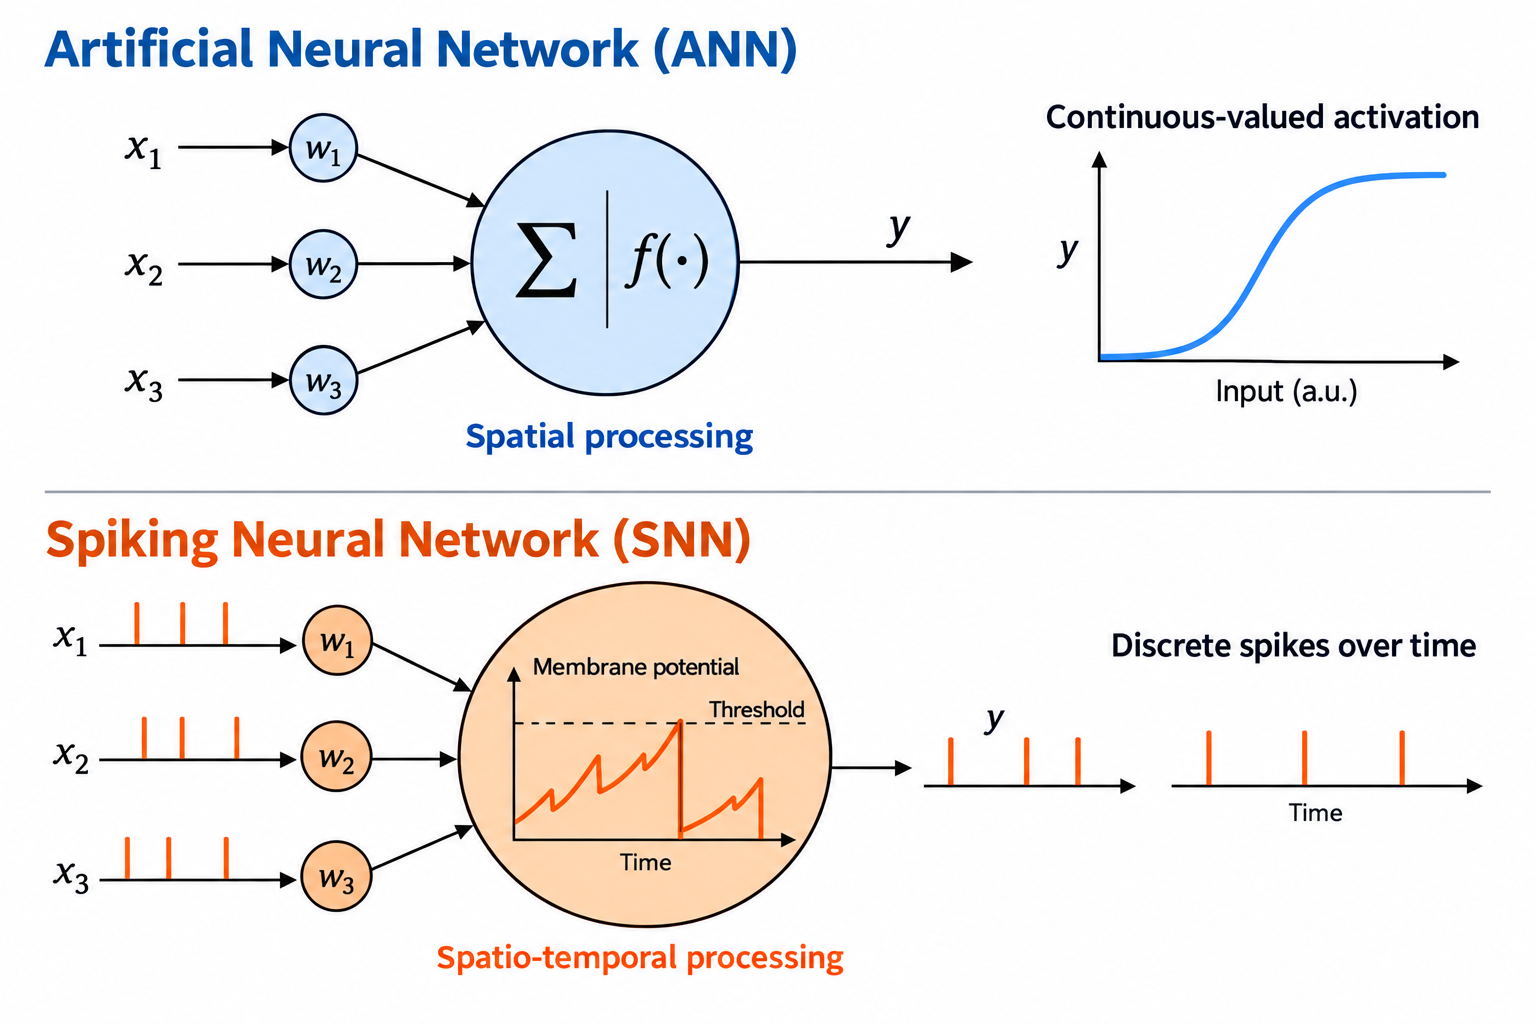
\includegraphics[width=.9\linewidth]{figures/ann_snn_comparison.png}
	\caption{Comparison of Information Processing in Artificial and Spiking Neurons}
	\label{fig:ann_snn_comparison}
\end{figure}

Figure \ref{fig:ann_snn_comparison} illustrates the main conceptual differences between a traditional artificial neuron and a spiking neuron. In an \gls{ann}, the weighted inputs are combined and transformed by an activation function, producing a continuous-valued output. The computation is mainly determined by the values presented to the neuron during a processing step. In an \gls{snn}, the inputs and outputs are represented by spike events distributed over time. Incoming spikes modify the membrane potential, which accumulates and gradually decays. When the membrane potential reaches the firing threshold, the neuron generates an output spike and its state is reset. Consequently, the behaviour of a spiking neuron depends not only on the presence of input events but also on their timing and the previous state of the neuron.

This distinction is often described as spatial processing in traditional \gls{ann}s and spatio-temporal processing in \gls{snn}s \cite{Maass1997}. The synaptic weights describe the spatial relationships between connected neurons, while the timing of spikes provides an additional temporal component. This does not imply that traditional neural networks cannot process temporal data. Instead, the difference concerns the fundamental communication mechanism and the explicit internal dynamics of the neuron model.

Information in an \gls{snn} can be encoded in several ways. In rate-based encoding, a larger input value is generally represented by a larger number of spikes within a defined time interval \cite{Gerstner2014}. In temporal encoding, information is represented by characteristics such as the time of the first spike or the relative timing between spikes \cite{Thorpe2001}. The selected encoding method influences the processing latency, spike activity, and complexity of the hardware implementation.

\gls{snn}s can be organized using network structures similar to those of traditional neural networks. For example, a feedforward \gls{snn} transfers spikes from an input layer through one or more processing layers to an output layer. Recurrent connections may also be included to preserve temporal information and model dynamic behaviour. In a classification task, the input data are first converted into spike trains and applied to the input neurons. The spikes propagate through weighted synapses to the output neurons, and the predicted class can be determined from their firing activity, for example, by identifying the neuron that produces the largest number of spikes during the observation period.

A major characteristic of \gls{snn}s is their event-driven operation \cite{Davis2018,Maass1997}. Computation is mainly triggered by the arrival of spikes rather than being performed continuously for every neuron and synapse. If spike activity is sufficiently sparse, inactive parts of the network do not need to perform synaptic operations \cite{Davis2018}. This property can reduce the number of computations and memory accesses. However, these potential advantages depend strongly on the network architecture, spike-encoding method, activity level, and hardware implementation. An inefficient implementation may not benefit from the sparsity of the spike events.

The event-driven and parallel characteristics of \gls{snn}s make them suitable for specialized hardware platforms \cite{Carpegna2025}. Neuromorphic processors, \gls{asic}s, and \gls{fpga}s can exploit parallelism between neurons and process spike events with deterministic latency. \Glspl{fpga} are particularly useful for \gls{snn} research because their configurable logic and memory resources allow different neuron models, numerical representations, and network structures to be implemented and evaluated without manufacturing a dedicated chip \cite{Carpegna2022}.

Despite their potential advantages, \gls{snn}s also present several challenges. Their temporal behaviour makes training and evaluation more complex than for traditional \gls{ann}s. Spike generation is non-differentiable, which prevents the direct application of standard gradient-based training methods without approximation. Hardware implementations must additionally manage neuron states, spike timing, synaptic memory, and communication between neurons. Supporting online learning further increases the complexity because synaptic weights must be updated during network operation instead of remaining fixed after offline training.

Therefore, the choice of neuron model and learning rule has an important effect on the computational complexity and hardware requirements of an \gls{snn}. Simplified neuron models are commonly used to retain the essential temporal behaviour of biological neurons while reducing implementation cost. The following sections introduce the spiking-neuron model and learning principles used as the theoretical basis of this work.

\section{Spiking Neuron Models}
\label{subsec: spiking neuron models}

Spiking-neuron models describe how neurons receive input spikes, update their internal states, and generate output spikes. Different models provide different levels of biological accuracy and computational complexity. The Hodgkin--Huxley model describes biological ion-channel dynamics in detail but requires several nonlinear differential equations \cite{HodgkinHuxley1952}. The Izhikevich model is computationally simpler while reproducing various biological firing patterns \cite{Izhikevich2003}. For digital hardware implementations, simplified models such as the \gls{if} and \gls{lif} models are more commonly used \cite{Gerstner2014}.

The \gls{lif} model provides a suitable compromise between biological plausibility and implementation efficiency. Its main state variable is the membrane potential \(V(t)\), which represents the electrical state of the neuron. Incoming spikes change the membrane potential according to their synaptic weights. In the absence of input, the membrane potential gradually returns towards its resting value. This behaviour is referred to as membrane leakage.

The membrane-potential dynamics of an \gls{lif} neuron are described by \cref{eq:lif-membrane-dynamics} \cite{Gerstner2014}.

\begin{equation}
    \tau_m \frac{\mathrm{d}V(t)}{\mathrm{d}t}
    =
    -\left(V(t)-V_{\mathrm{rest}}\right)
    + R_m I(t)
    \label{eq:lif-membrane-dynamics}
\end{equation}

where \(\tau_m\) is the membrane time constant, \(V_{\mathrm{rest}}\) is the resting potential, \(R_m\) is the membrane resistance, and \(I(t)\) represents the total input current. The leakage term causes the membrane potential to decay over time, while the input current term increases or decreases it in response to synaptic events.

The total synaptic input is determined by the received presynaptic spikes and their associated weights, as shown in \cref{eq:total-input-current} \cite{Gerstner2014}.

\begin{equation}
    I(t)
    =
    \sum_{i} w_i s_i(t)
    \label{eq:total-input-current}
\end{equation}

where \(w_i\) is the weight of synapse \(i\), and \(s_i(t)\) indicates the occurrence of a presynaptic spike. Excitatory synapses increase the membrane potential, whereas inhibitory synapses decrease it. Because spikes can be represented as binary events, synaptic processing can often be implemented using additions and subtractions rather than general multiplication operations.

\begin{figure}[t]
	\centering
	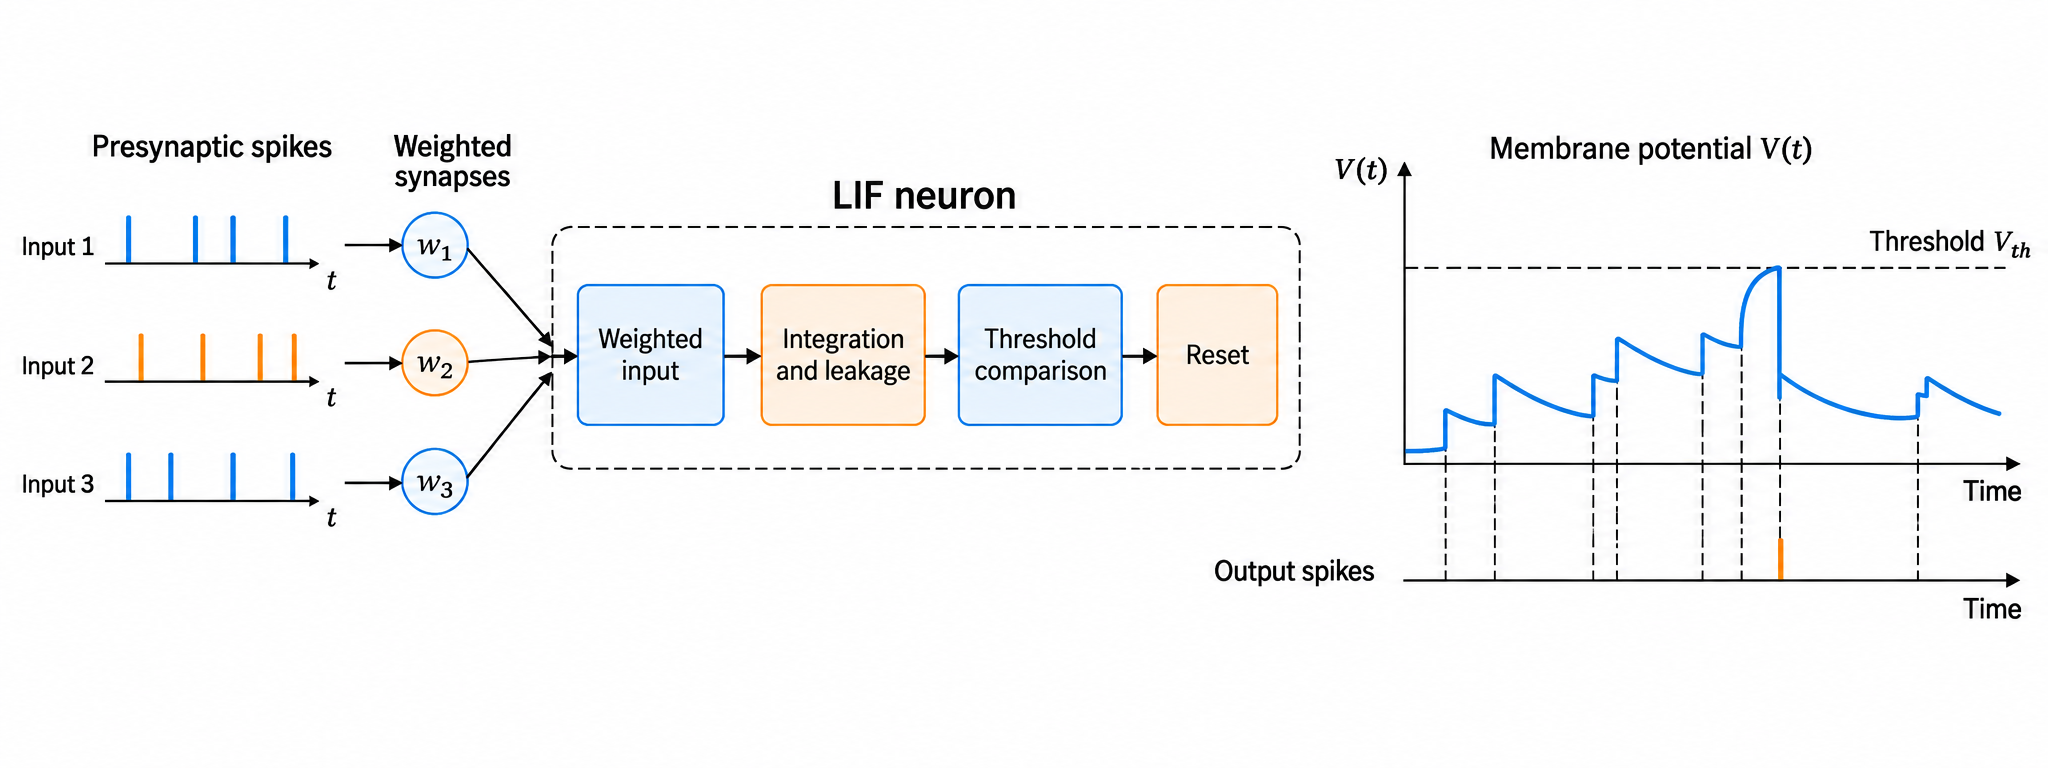
\includegraphics[width=.98\linewidth]{figures/lif_neuron_model.png}
	\caption{\gls{lif} Neuron Model Operating Principle}
	\label{fig:lif-neuron-model}
\end{figure}

Figure \ref{fig:lif-neuron-model} illustrates the operating principle of the \gls{lif} neuron model. Each presynaptic spike produces a weighted change in the membrane potential. Between input events, the potential decreases because of leakage. When several input spikes arrive within a sufficiently short interval, their effects accumulate and may cause the membrane potential to reach the firing threshold \(V_{\mathrm{th}}\). The output of the neuron can be represented as

\begin{equation}
    s_{\mathrm{out}}(t)
    =
    \begin{cases}
        1, & V(t) \geq V_{\mathrm{th}} \\
        0, & V(t) < V_{\mathrm{th}}
    \end{cases}
    \label{eq:output-spike-generation}
\end{equation}

After an output spike is generated, the neuron state must be reset. In a hard-reset model, the membrane potential is directly set to a predefined reset value. In a subtractive-reset model, the firing threshold is subtracted from the membrane potential:

\begin{equation}
    V(t) \leftarrow V(t) - V_{\mathrm{th}}
    \label{eq:subtractive-reset}
\end{equation}

Unlike a hard reset, the subtractive reset preserves the portion of the membrane potential that exceeds the firing threshold \cite{Rueckauer2017}. This remaining potential can contribute to subsequent spike generation. A refractory period may also be introduced to prevent the neuron from firing again immediately after an output spike.

For implementation in synchronous digital hardware, the continuous-time equation is converted into a discrete-time form. A simplified representation is

\begin{equation}
    V[k+1]
    =
    \alpha V[k]
    +
    \sum_{i} w_i s_i[k]
    \label{eq:discrete-membrane-update}
\end{equation}

where \(k\) denotes the current time step and \(\alpha\) is a decay factor representing membrane leakage. After the membrane potential is updated, it is compared with the firing threshold. If the threshold is reached, an output spike is generated and the reset operation is applied.

This discrete formulation mainly requires registers, adders, comparators, and simple leakage logic, making the \gls{lif} model well suited to \gls{fpga} implementation \cite{Carpegna2025}. Fixed-point or integer arithmetic can be used instead of floating-point arithmetic to reduce hardware complexity. The selected bit width and numerical precision influence both the accuracy of the neuron dynamics and the required hardware resources.

In this work, an \gls{lif} neuron model with subtractive reset is used as the processing element of the \gls{snn}. In addition to determining the generation of output spikes, its membrane potential is used by the \gls{sdsp} learning rule to control synaptic weight updates, which will be introduced in the following sections.

\section{Learning in Spiking Neural Networks}
\label{subsec: learning in spiking neural networks}

Learning enables an \gls{snn} to adapt its synaptic weights according to input data, neuronal activity, or external feedback. During inference, synaptic weights remain fixed and the network only processes incoming spikes. During learning, the weights are modified so that the network can adapt its response to particular input patterns. Because \gls{snn}s process information through discrete spikes and time-dependent neuron states, their learning mechanisms must consider not only neuronal activation but also the timing and sequence of spike events \cite{Gerstner2014,Neftci2019}.

This section first introduces the main learning approaches used in \gls{snn}s. It then focuses on \gls{sdsp}, which is the local online learning rule implemented in this work.

\subsection{Learning Approaches for Spiking Neural Networks}
\label{subsec: learning approaches for snns}

\gls{snn} learning methods can first be classified according to whether weight adaptation is performed offline or online. In offline learning, the network is trained before being deployed on the target hardware. Training can therefore be performed using \gls{cpu} or \gls{gpu}, and the resulting weights are subsequently transferred to the hardware accelerator. During normal hardware execution, these weights remain fixed. This approach avoids the additional control logic and writable weight storage required for training, but it prevents the deployed system from independently adapting to new data or changing operating conditions.

In online learning, synaptic weights are updated while the \gls{snn} is operating. The learning rule is evaluated directly from the observed network activity, allowing the system to adapt after deployment. However, the relevant neuron states must be available to the learning circuit, and inference and learning operations must be coordinated when accessing the same synaptic memory \cite{Frenkel2019ODIN}.

Learning methods can also be classified according to the source of the learning signal. In supervised learning, the desired output or class label is known during training, and the difference between the observed and desired output is used to guide the weight updates. In unsupervised learning, no explicit target output is available. Instead, synaptic weights are modified according to statistical patterns or correlations in the neuronal activity. Reinforcement learning uses a reward or penalty to evaluate the behaviour of the network without specifying the desired activity of every individual neuron \cite{Neftci2019}.

These classifications describe different aspects of the learning process and should not be considered mutually exclusive. For example, supervised learning may be performed offline using a gradient-based training algorithm or online using a teacher signal. Similarly, an unsupervised local rule may be implemented directly in hardware or simulated offline during network development.

Traditional \gls{ann}s are commonly trained using backpropagation and gradient descent. Applying these methods directly to \gls{snn}s is difficult because the spike-generation function is discontinuous. For a deterministic spiking neuron, its derivative is zero almost everywhere and undefined at the firing threshold. Consequently, the standard gradient cannot be propagated directly through the spike function. Surrogate-gradient methods address this problem by replacing the derivative of the spike function with a smooth approximation during training \cite{Neftci2019}. Such methods can train multilayer \gls{snn}s effectively, but they generally require error propagation and the storage of intermediate neuron states, which complicates direct online hardware implementation \cite{Zenke2018}.

Local learning rules provide an alternative approach. A local rule updates a synaptic weight using information that is available at or close to the corresponding synapse. This information may include presynaptic spikes, postsynaptic spikes, membrane potential, or a local activity trace. Because a complete error gradient does not need to be propagated through the network, local rules can reduce communication and memory requirements.

\gls{stdp} is a well-known example of local synaptic learning. In its basic form, the direction of the weight change depends on the relative timing of presynaptic and postsynaptic spikes. A presynaptic spike occurring shortly before a postsynaptic spike commonly causes synaptic potentiation, whereas the opposite order commonly causes synaptic depression \cite{BiPoo1998}. Evaluating \gls{stdp} requires information about the timing difference between the two spike events.

For resource-constrained online-learning hardware, local rules that require only a small number of neuron-state variables are particularly attractive. \gls{sdsp} follows this principle by triggering weight-update decisions on presynaptic spike events and determining the update direction from the current postsynaptic neuron state \cite{Brader2007}. The rule is described in detail in Section \ref{subsec: sdsp}.

\subsection{Spike-Driven Synaptic Plasticity}
\label{subsec: sdsp}

\gls{sdsp} was introduced by Brader, Senn, and Fusi as a local learning mechanism for networks that learn temporal spike patterns \cite{Brader2007}. The rule was designed so that synaptic updates depend only on information locally available at the synapse and the postsynaptic neuron. It therefore avoids the backward propagation of a global error signal and is suitable for event-driven online learning.

An \gls{sdsp} update is evaluated when a presynaptic spike arrives. At that moment, the rule observes the postsynaptic membrane potential and a calcium-related activity variable. The membrane potential describes the current state of the postsynaptic neuron, while the calcium variable provides an estimate of its recent firing activity. These two variables determine whether the active weight should be increased, decreased, or left unchanged \cite{Brader2007,Frenkel2019ODIN}.

The calcium variable \(C(t)\) can be represented as an activity trace that increases when the postsynaptic neuron produces a spike and decreases over time. A general continuous-time representation is

\begin{equation}
    \frac{\mathrm{d}C(t)}{\mathrm{d}t}
    =
    -\frac{C(t)}{\tau_C}
    +
    J_C \sum_{k}
    \delta\left(t-t_k^{\mathrm{post}}\right)
    \label{eq:calcium-dynamics}
\end{equation}

where \(\tau_C\) is the calcium decay time constant, \(J_C\) is the increase caused by a postsynaptic spike, and \(t_k^{\mathrm{post}}\) denotes the occurrence time of the \(k\)-th postsynaptic spike \cite{Brader2007}. Consequently, a high calcium value indicates strong recent postsynaptic activity, whereas a low value indicates limited activity.

In a digital implementation, the continuous calcium variable can be approximated using a counter. The counter is incremented when a postsynaptic spike occurs and decremented when a leakage event is received. This replaces continuous decay with discrete state updates and avoids the need for complex arithmetic. The calcium value is then compared with a set of programmable thresholds \cite{Frenkel2019ODIN}.

A commonly used hardware-oriented formulation of the \gls{sdsp} update rule can be expressed as

\begin{equation}
    \Delta w
    =
    \begin{cases}
        +1,
        & V_{\mathrm{mem}}\left(t_{\mathrm{pre}}\right) > \theta_m
          \ \text{and}\
          \theta_1 < C\left(t_{\mathrm{pre}}\right) < \theta_3
        \\[2pt]
        -1,
        & V_{\mathrm{mem}}\left(t_{\mathrm{pre}}\right) \leq \theta_m
          \ \text{and}\
          \theta_1 < C\left(t_{\mathrm{pre}}\right) < \theta_2
        \\[2pt]
        0,
        & \text{otherwise}
    \end{cases}
    \label{eq:sdsp-weight-update}
\end{equation}

where \(t_{\mathrm{pre}}\) is the arrival time of the presynaptic spike, \(V_{\mathrm{mem}}\) is the postsynaptic membrane potential, \(\theta_m\) is the membrane-potential threshold, and \(\theta_1\), \(\theta_2\), and \(\theta_3\) are calcium thresholds with \(\theta_1 < \theta_2 < \theta_3\) \cite{Frenkel2019ODIN}.

When the membrane potential is above \(\theta_m\), the postsynaptic neuron is considered sufficiently activated. If the calcium value is also within the potentiation interval, the synaptic weight is increased. When the membrane potential is below or equal to \(\theta_m\) and the calcium value is within the depression interval, the weight is decreased. In all other cases, the weight remains unchanged.

The calcium thresholds prevent learning when the postsynaptic neuron is either insufficiently active or excessively active. The lower threshold \(\theta_1\) prevents updates when the recent postsynaptic activity is too low. The upper thresholds \(\theta_2\) and \(\theta_3\) define the activity ranges in which depression and potentiation are permitted. This behaviour acts as a stop-learning mechanism and limits continuous weight modification outside the desired activity range \cite{Brader2007}.

Figure \ref{fig:conceptual-operation-of-sdsp} summarizes the information flow of the \gls{sdsp} learning rule.

\begin{figure}[t]
	\centering
	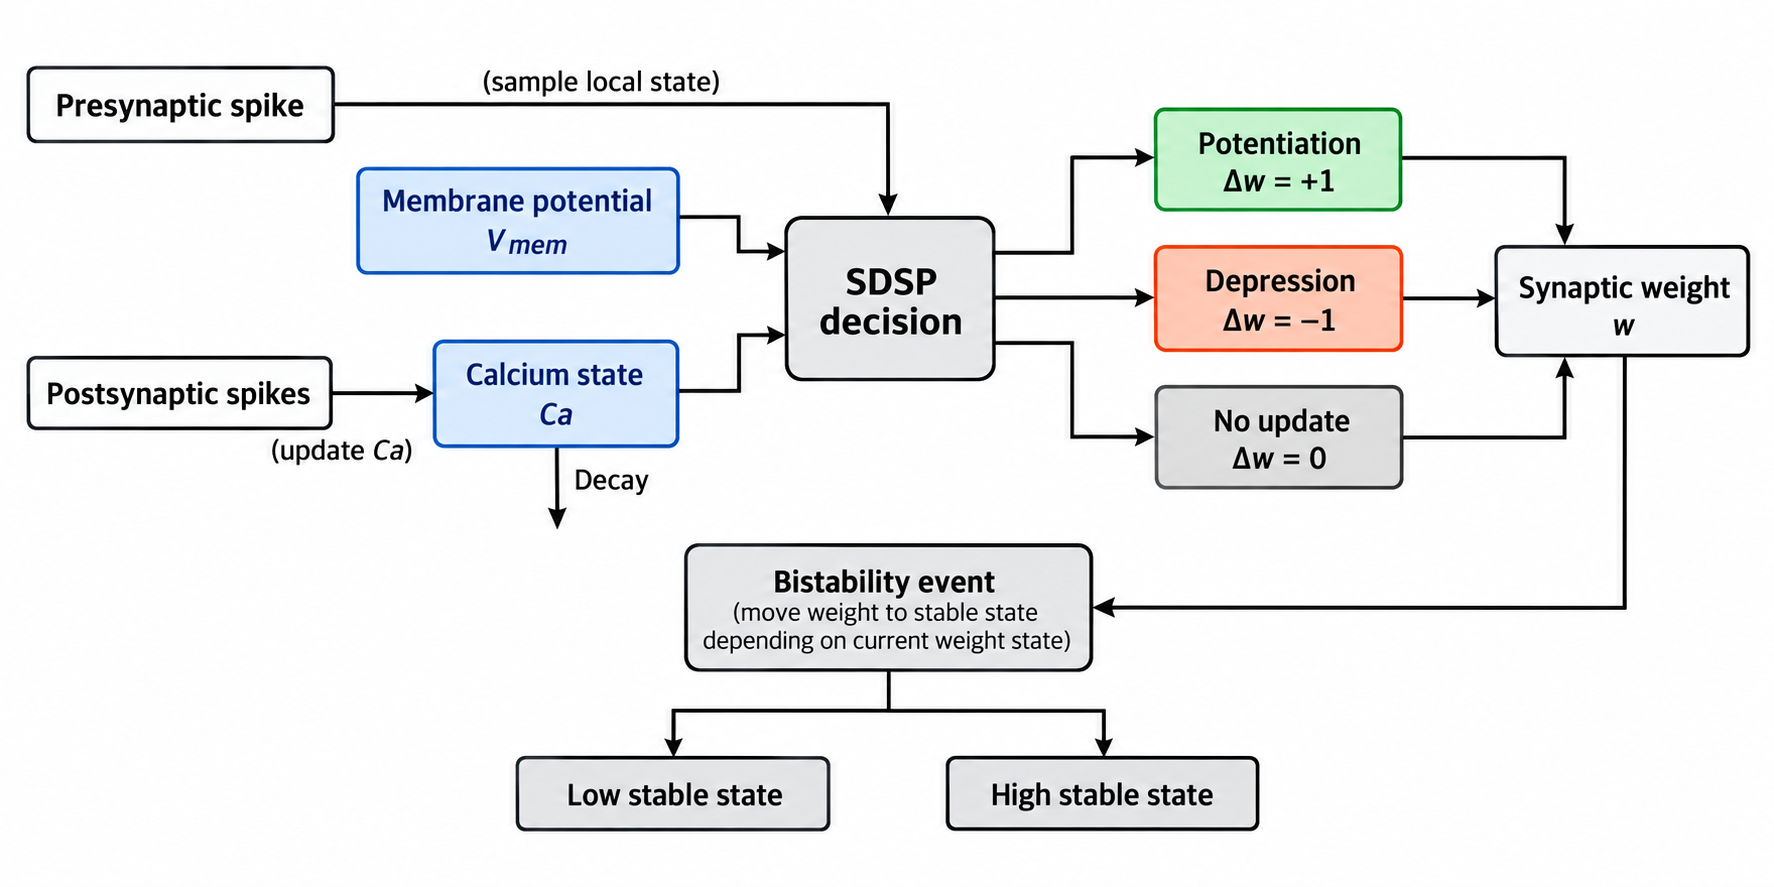
\includegraphics[width=.9\linewidth]{figures/sdsp_learning_rule.png}
	\caption{\gls{sdsp} Weight-Update Decisions and Bistability Mechanism}
	\label{fig:conceptual-operation-of-sdsp}
\end{figure}

\gls{sdsp} also includes a bistability mechanism. In the absence of a spike-driven update, the synaptic state gradually moves towards either a low or a high stable state. In the original formulation, this behaviour can be represented as

\begin{equation}
    \frac{\mathrm{d}w}{\mathrm{d}t}
    =
    \begin{cases}
        +\alpha, & w > \theta_w, \\
        -\beta,  & w \leq \theta_w
    \end{cases}
    \label{eq:synaptic-weight-drift}
\end{equation}

where \(\theta_w\) separates the two attraction regions, and \(\alpha\) and \(\beta\) determine the corresponding drift rates \cite{Brader2007}. This mechanism reduces the likelihood that a synaptic weight remains indefinitely in an unstable intermediate state.

In digital hardware, bistability can be implemented using periodic update events. When such an event occurs, the weight is incremented if it belongs to the upper region and decremented if it belongs to the lower region. The update continues until the weight reaches one of its numerical boundaries. With an unsigned binary representation, the most significant weight bit can be used to distinguish the two regions, avoiding a separate numerical comparison.

The \gls{sdsp} rule is suitable for hardware implementation because it requires only local state variables, threshold comparisons, and bounded weight increments or decrements. It does not require multiplication, global gradient computation, or the storage of precise presynaptic-to-postsynaptic timing differences. Digital processors such as ODIN have demonstrated that \gls{sdsp} can be implemented using time-multiplexed learning logic and on-chip writable synaptic memory \cite{Frenkel2019ODIN}.

In this work, the hardware-oriented \gls{sdsp} rule is adapted for integration with the \gls{snn} generated by Spiker+. The membrane potential and calcium state are represented using finite-width digital values, while the synaptic weights are modified using bounded integer updates. The exact numerical representation, threshold selection, control signals, and \gls{rtl} architecture are design-specific choices and are therefore presented later in Chapter \ref{sec:design_methodology} and Chapter \ref{sec:implementation}.

\section{FPGA-Based Neural Network Acceleration}
\label{subsec: fpga-based neural network acceleration}

\gls{fpga}s are reconfigurable integrated circuits whose hardware functionality can be defined after manufacturing. In contrast to processors that execute instructions sequentially, an \gls{fpga} allows application-specific datapaths and control structures to be implemented directly in hardware. This enables operations to be executed concurrently and makes \gls{fpga}s suitable for applications requiring low latency, deterministic timing, and adaptable hardware architectures.

\gls{fpga}s occupy a useful position between general-purpose processors and \gls{asic}s. \gls{cpu}s and \gls{gpu}s provide a convenient programming environment but execute applications on a predefined architecture. \gls{asic}s can offer higher efficiency, but their functionality is fixed after fabrication and their development requires considerable time and cost. \gls{fpga}s retain hardware-level parallelism while allowing the design to be modified and reprogrammed. These characteristics make them suitable for the development and evaluation of \gls{snn} accelerators \cite{Karamimanesh2025}.

A simplified overview of the main \gls{fpga} resources is shown in Figure \ref{fig:fpga-architecture-overview}. The main computational resources of an \gls{fpga} are configurable logic blocks. These blocks contain \gls{lut}s and \gls{ff}s that can be configured to implement combinational and sequential logic. \gls{lut}s can realize Boolean functions and small arithmetic operations, while \gls{ff}s store intermediate values and system states. Together, these resources can implement neuron update logic, comparators, counters, state machines, and learning-rule control circuits \cite{UG474}.

\begin{figure}[t]
	\centering
	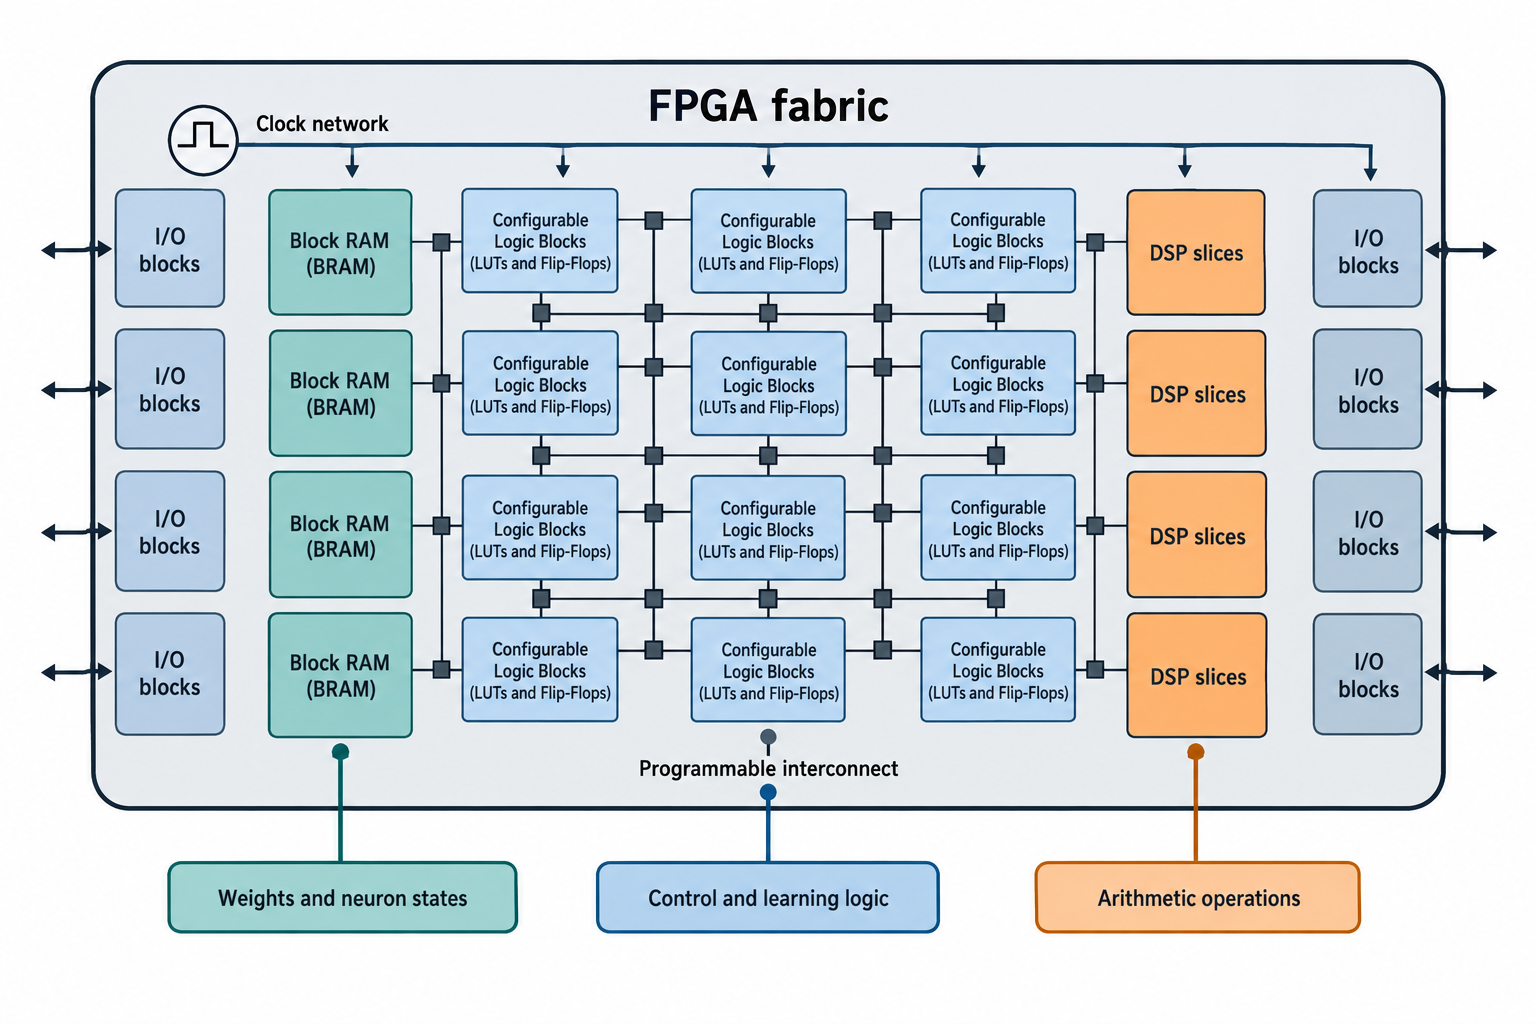
\includegraphics[width=.9\linewidth]{figures/fpga_architecture_overview.png}
	\caption{Principal \gls{fpga} Resources for \gls{snn} Acceleration}
	\label{fig:fpga-architecture-overview}
\end{figure}

Modern \gls{fpga}s also contain dedicated on-chip memory resources, commonly referred to as \gls{bram}. \gls{bram} provides larger and more structured storage than registers implemented using \gls{ff}s. In an \gls{snn} accelerator, it can be used to store synaptic weights, neuron membrane potentials, thresholds, input spikes, and intermediate network states. Since memory access often determines the performance and scalability of a neural-network accelerator, the organization of these memories is an important architectural decision \cite{UG473}.

Dedicated \gls{dsp} slices are provided for arithmetic operations such as multiplication, addition, and accumulation \cite{UG479}. They are particularly useful for traditional neural networks, which frequently require large numbers of multiply-accumulate operations. However, an \gls{snn} may require fewer multiplications because spikes are typically represented as binary events. Synaptic integration and local learning rules can often be implemented using additions, comparisons, and conditional updates. Depending on the selected neuron and learning models, these operations may therefore be implemented using configurable logic without requiring a large number of \gls{dsp} slices.

The parallel and configurable nature of an \gls{fpga} matches the computational characteristics of \gls{snn}s. Multiple neurons or synapses can be updated concurrently by allocating separate hardware resources to them. Alternatively, a smaller number of processing units can be reused across several neurons through time multiplexing. A fully parallel architecture can reduce processing latency but requires more hardware resources, whereas a time-multiplexed architecture reduces resource consumption at the cost of additional execution cycles. \gls{fpga}-based \gls{snn} design therefore involves a trade-off between resource utilization, latency, throughput, and supported network size.

An \gls{fpga} design is commonly described using a \gls{hdl} such as VHDL or Verilog. The \gls{rtl} description is first verified through simulation and then transformed into a hardware netlist through synthesis \cite{UG901}. During implementation, the synthesized logic is mapped to physical \gls{fpga} resources, placed on the device, and connected through the programmable routing network. After timing requirements have been verified, a configuration bitstream is generated and loaded onto the \gls{fpga} \cite{UG904}.

The main evaluation metrics for an \gls{fpga}-based neural network accelerator include the utilization of \gls{lut}s, \gls{ff}s, \gls{bram}, and \gls{dsp} slices. Timing characteristics such as maximum clock frequency, processing latency, and throughput are also important. In applications targeting embedded or edge systems, power consumption and energy efficiency may additionally be considered. These metrics allow different hardware architectures and resource-sharing strategies to be compared.

In this thesis, the Spiker+ framework is used as the basis for generating an \gls{fpga}-based \gls{snn} accelerator \cite{Carpegna2025}. The original inference-oriented architecture is extended with \gls{sdsp}-based online learning, which requires writable synaptic-weight storage and additional control logic for weight updates. \gls{fpga} technology makes it possible to integrate these functions into a customized hardware architecture while retaining the ability to modify the implementation. Its reconfigurable nature also motivated an assessment of whether learning functions could be exchanged at runtime. The following section introduces the \gls{dpr} concepts required for that assessment; Section \ref{subsec:dpr-applicability} explains why \gls{dpr} was excluded from the final implementation.

\section{Dynamic Partial Reconfiguration}
\label{subsec: dynamic partial reconfiguration}

\gls{fpga}s can be reprogrammed after manufacturing by loading configuration data into the device. In a conventional configuration process, a complete bitstream defines the functionality of the entire programmable logic. Loading a new full bitstream replaces the complete hardware design and normally interrupts all functions implemented in the \gls{fpga} fabric. Partial reconfiguration provides a more flexible alternative by modifying only a selected region of the device while leaving the remaining logic unchanged \cite{VipinFahmy2018}.

When partial reconfiguration is performed during system operation, it is commonly referred to as \gls{dpr}. AMD/Xilinx currently uses the term \gls{dfx} for this technology. Both terms describe the ability to exchange hardware functionality within a predefined region without reconfiguring the complete \gls{fpga} \cite{UG909}. In this thesis, the term \gls{dpr} is used as the general technological concept.

A \gls{dfx} design is divided into a static region and one or more reconfigurable partitions. The static region contains logic that remains configured throughout system operation, such as communication interfaces, memories, system controllers, and functions that must remain continuously available. A Reconfigurable Partition (RP) is a physically defined region of the \gls{fpga} reserved for dynamically replaceable functionality. The alternative hardware functions that can be loaded into this region are referred to as \glspl{rm} \cite{UG909}.

Each \gls{rm} may implement different functionality, but all modules assigned to the same \gls{rp} must use a compatible boundary interface. The interface defines the signals exchanged between the static logic and the reconfigurable module. The physical size of the \gls{rp} must also be sufficient for the largest \gls{rm} because every alternative module must be placed and routed within the same reserved \gls{fpga} region \cite{UG909,VipinFahmy2018}.

\begin{figure}[t]
	\centering
	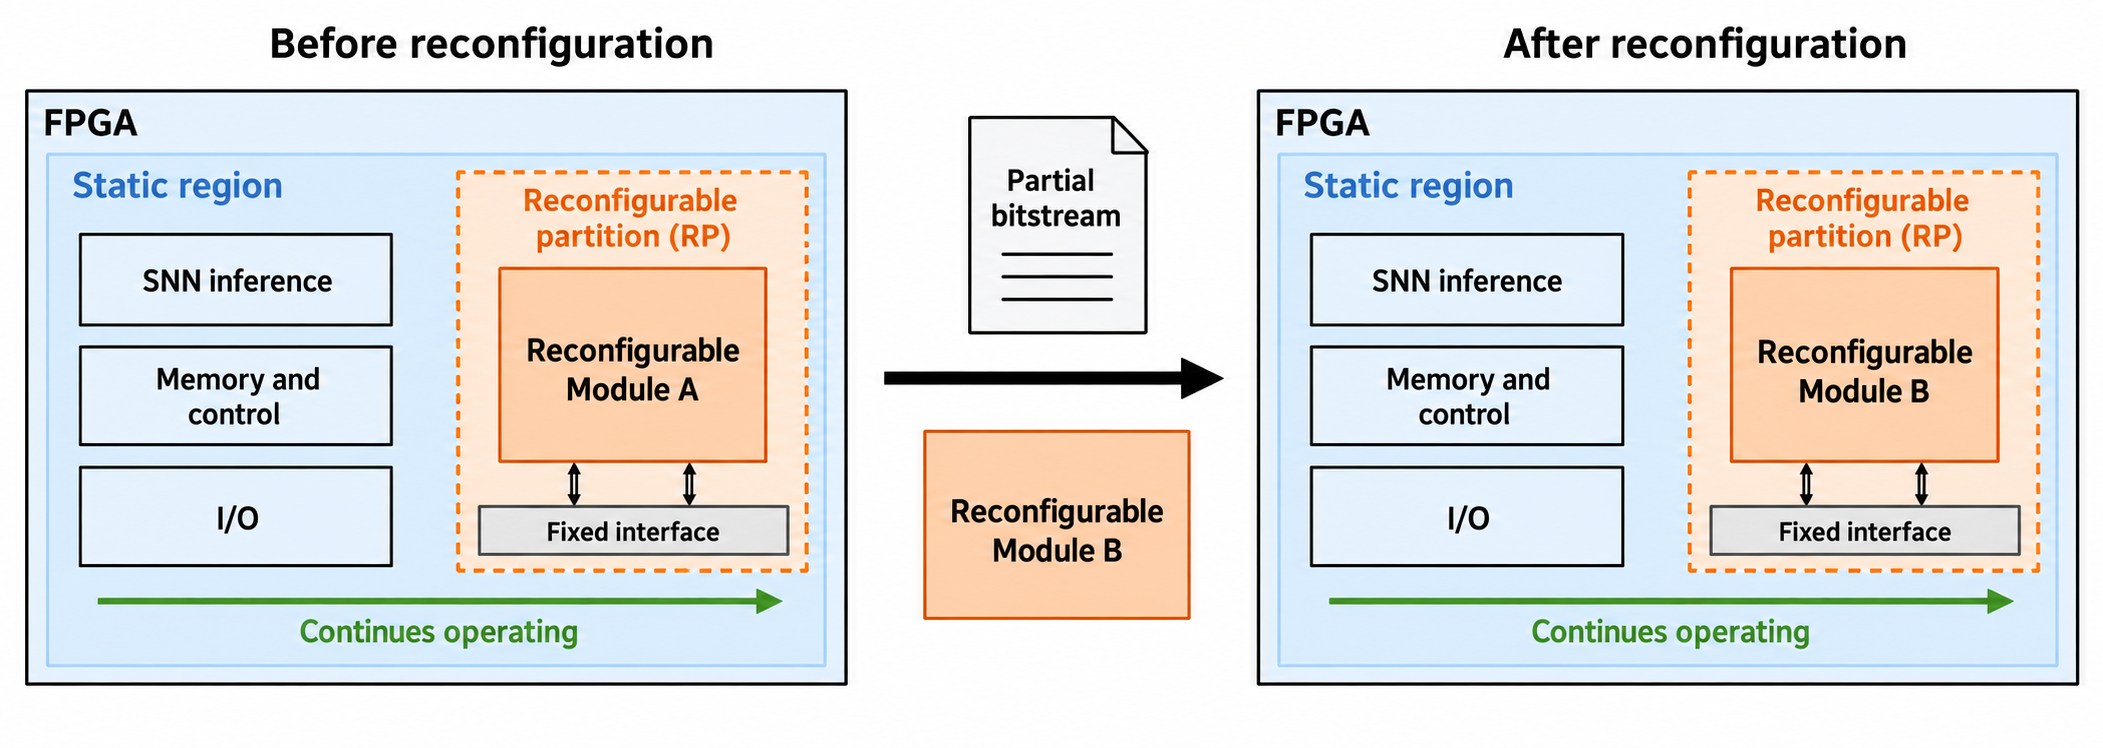
\includegraphics[width=.9\linewidth]{figures/dynamic_partial_reconfiguration.png}
	\caption{Basic Operating Principle of \gls{dpr}}
	\label{fig:basic-operating-principle-of-dpr}
\end{figure}

As shown in Figure \ref{fig:basic-operating-principle-of-dpr}, the initial \gls{fpga} configuration contains the static region and Reconfigurable Module A. To change the functionality, a partial bitstream containing the configuration data for Reconfigurable Module B is transferred to the \gls{fpga} configuration interface. Only the configuration frames associated with the \gls{rp} are modified. After the partial bitstream has been loaded, Module B occupies the same physical region and communicates with the static design through the same boundary interface.

The static region can continue operating during this process. However, the \gls{rp} itself is temporarily unavailable, and its output signals may be undefined while its configuration memory is being modified. Logic connected to the \gls{rp} must therefore not use these signals during reconfiguration. A decoupling mechanism can isolate the \gls{rp} boundary, while a controller stops new transactions, initiates the reconfiguration, waits for completion, and reconnects the new module afterwards \cite{UG909}. Therefore, \gls{dpr} does not guarantee that every function in the system continues without interruption; it allows the unaffected static logic to remain operational while the selected partition is temporarily replaced.

The \gls{dpr} implementation flow begins by separating the design hierarchy into static and reconfigurable components. An \gls{rp} is assigned to a physical region of the \gls{fpga} through floorplanning constraints, and each \gls{rm} is synthesized and implemented for this region. The static logic and \gls{rp} boundary must remain consistent across all configurations. The completed implementations are then verified for compatibility before full and partial bitstreams are generated \cite{UG909}.

A full bitstream is initially required to configure the complete device, including the static design and an initial \gls{rm}. During runtime, partial bitstreams are used to exchange only the content of the \gls{rp}. Depending on the \gls{fpga} platform, these bitstreams may be transferred through configuration interfaces such as the \gls{icap}, \gls{pcap}, JTAG, or another supported configuration path \cite{UG909}.

\section{Spiker+ Framework}
\label{subsec: spiker framework}

Spiker+ is an open-source framework for configuring, training, quantizing, and generating \gls{fpga} accelerators for \gls{snn} inference. It builds on the original Spiker accelerator, which introduced an FPGA-oriented, fixed-point architecture based on parallel neuron updates, sequential input-spike processing, and simplified \gls{lif} arithmetic \cite{Carpegna2022}. The original design demonstrated that these choices could reduce the hardware cost of an SNN accelerator, but it was developed primarily as a task-specific inference architecture. Spiker+ generalizes this foundation into a Python-controlled generation framework so that a user can describe an SNN at a higher abstraction level instead of manually constructing its complete \gls{rtl} hierarchy \cite{Carpegna2025}.

\subsection{Supported Design Space}

The built-in design space includes fully connected feedforward and recurrent networks. Its neuron library provides \gls{if}, first-order \gls{lif}, and second-order \gls{lif} models, each with either a fixed-reset or subtractive-reset implementation. A Python dictionary describes the selected network architecture, the number and size of its layers, the neuron model and parameters, the number of temporal processing steps, and the required feedback connections. The framework's network-builder module converts this description into a Python network object that is subsequently used by the training, optimization, and hardware-generation stages \cite{Carpegna2025}.

This separation between the high-level network description and the generated hardware is an important property of Spiker+. Network-level choices are expressed in Python, whereas implementation details such as control-unit instantiation, neuron datapaths, synchronization, and parameter initialization are produced by the generator. The framework is nevertheless not a general compiler for every possible SNN topology: its built-in generation flow targets the network structures and neuron models provided by its component library \cite{Carpegna2025}.

\subsection{Configuration and Generation Flow}

The complete Spiker+ configuration and generation process is illustrated in Figure \ref{fig:spikerplus-configuration-framework}. The flow consists of four principal stages: network construction, software training, numerical optimization, and VHDL generation \cite{Carpegna2025}.

\begin{figure}[t]
	\centering
	\makebox[\linewidth][c]{%
		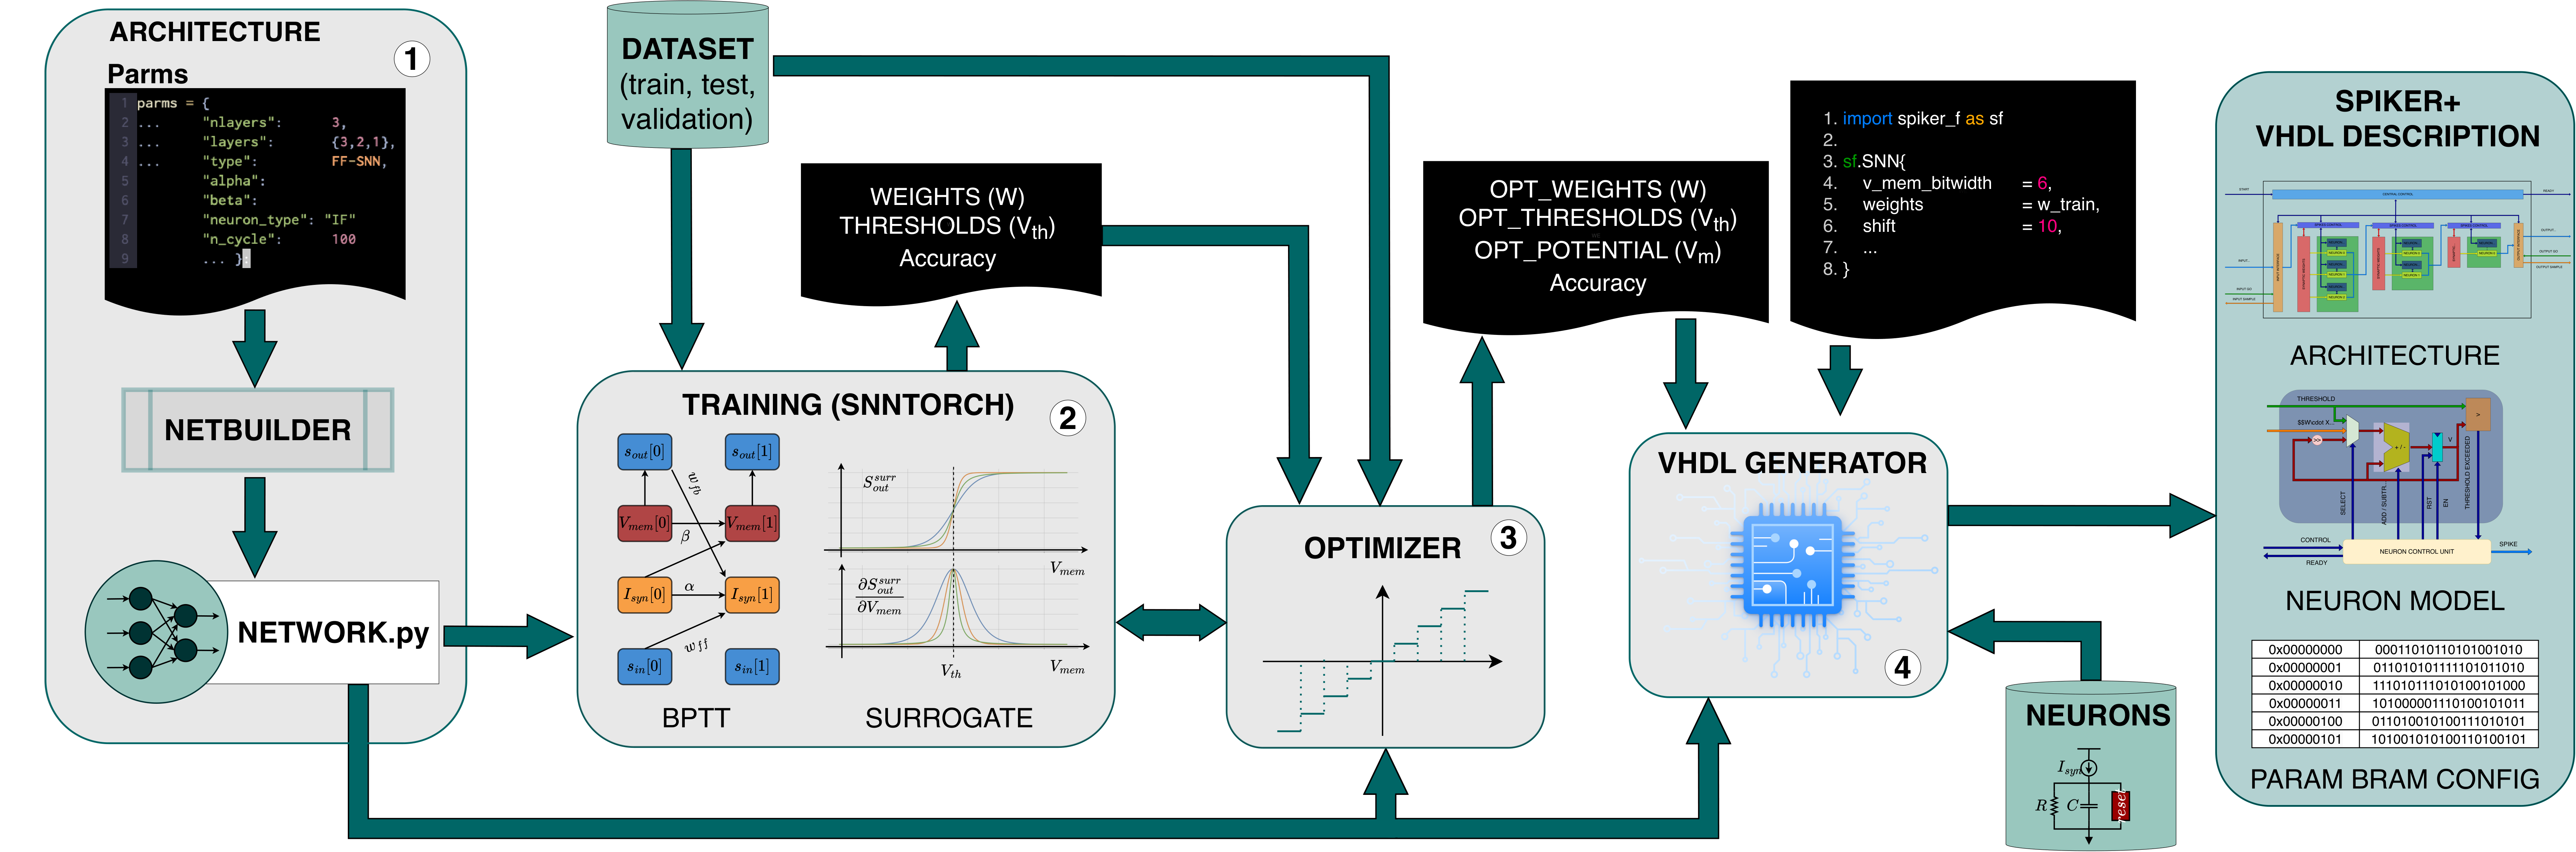
\includegraphics[width=1.10\linewidth]{figures/spikerplus_configuration_framework_original.png}%
	}
	\caption{Spiker+ Configuration, Optimization, and VHDL Generation Workflow \cite{Carpegna2025}}
	\label{fig:spikerplus-configuration-framework}
\end{figure}

In the first stage, the network builder creates the configured software model. The second stage trains this model using the framework's built-in integration with snnTorch and PyTorch. The training process produces the synaptic weights, firing thresholds, and other neuron parameters used during inference. Hardware-oriented approximations, such as restricting constant decay factors to shift-compatible values, can already be considered during training so that the software model reflects the arithmetic later used by the accelerator \cite{Carpegna2022,Carpegna2025}.

The third stage converts the floating-point training result into a signed \(N\)-bit fixed-point representation. Values outside the representable range are saturated, and the framework can evaluate several quantization widths to determine how reduced precision affects inference accuracy. This exploration is relevant because weight and membrane-potential widths influence both memory consumption and arithmetic cost. Reducing the weight width can also increase the number of weights obtained from an on-chip memory access, but the selected representation must retain sufficient numerical accuracy for the target network \cite{Carpegna2025}.

In the fourth stage, the VHDL generator translates the selected network object and its quantized parameters into synthesizable modules. It also produces parameter-initialization files for the synaptic memories and a file-driven testbench for simulation. The generated output is therefore not merely a parameter file for a fixed accelerator: it is a network-specific VHDL hierarchy that can subsequently be synthesized and implemented for the selected \gls{fpga} \cite{Carpegna2025}.

\subsection{Generated Hardware Architecture}

The generated accelerator follows three control levels. A Network Control Unit coordinates the temporal evolution of the complete network and synchronizes the layers and external interfaces. Each Layer Control Unit supplies the input spikes associated with one layer and waits for its neurons to complete the requested operation. At the lowest level, a Neuron Control Unit sequences the operations performed by its Neuron Datapath, including synaptic integration, leakage, threshold comparison, firing, and reset. Communication between adjacent blocks uses a two-signal \texttt{start}/\texttt{ready} handshake, which keeps the hierarchy modular and allows a controller to wait until all participating blocks have completed their current operation \cite{Carpegna2025}.

Spiker+ deliberately combines spatial parallelism with temporal reuse. All neurons in a layer can process the currently selected presynaptic input in parallel, whereas the individual inputs connected to that layer are supplied sequentially. The temporal steps of the spike train are also evaluated in sequence because each step depends on the evolving neuron state. This organization avoids instantiating one arithmetic datapath for every synapse while retaining parallel execution across the postsynaptic neurons. When no input spike is active in a time step, the layer controller can skip the otherwise unnecessary scan of its input connections, allowing sparse spike activity to reduce latency and switching activity \cite{Carpegna2022,Carpegna2025}.

The neuron datapaths exploit properties of the SNN model to simplify the arithmetic. Because a spike is binary, multiplying a synaptic weight by a spike becomes a conditional selection between zero and the weight. Fixed-point decay factors that are chosen as, or approximated by, powers of two allow constant multiplications to be replaced by shifts. These transformations reduce the need for general multipliers while preserving the neuron operations represented by the trained software model \cite{Carpegna2022,Carpegna2025}.

Synaptic weights are quantized and initialized from generated files. For the on-chip implementation, weights can be stored in \gls{bram}, whose independent memory blocks provide the bandwidth required to supply the weights of several neurons in parallel. Spiker+ also defines a synapse interface based on the same \texttt{start}/\texttt{ready} protocol, allowing an alternative memory organization to deliver the current weights before the layer proceeds. Using external memory can increase capacity, but the transfer required before each operation reduces the achievable accelerator speed \cite{Carpegna2025}.

The framework leaves the board-specific input and output implementation outside the generated neural core. Inputs may already be encoded as spike streams or may be converted from numerical data by a separate encoding block. At the output, the firing activity of the final layer can be accumulated and post-processed, for example by selecting the neuron with the largest spike count. The external interfaces must follow the accelerator's handshake protocol, but their concrete realization depends on the surrounding system \cite{Carpegna2025}. This boundary is used in Chapter \ref{sec:implementation}, where the generated network is connected to an AXI-based PYNQ data path.

\subsection{Relevance to This Thesis}

Spiker+ provides the baseline network hierarchy, neuron arithmetic, synchronization, and generated parameter memories used in this work. However, the framework version considered here targets inference with parameters obtained through offline training. Its generated synaptic weights are initialized for read access and remain fixed during network execution. Online learning consequently requires changes below the Python configuration level: the neuron state must be exposed to the learning rule, the excitatory memory must support runtime writes, and the layer schedule must retain the association between each update and its original synaptic address. Chapters \ref{sec:design_methodology} and \ref{sec:implementation} describe how these extensions are introduced while retaining the principal Spiker+ hierarchy and handshake structure.

% !TEX root = thesis.tex
\chapter{Related Work}
\label{sec:related_work}

This chapter reviews representative digital hardware architectures that support on-chip or online learning in \gls{snn}s. The selected works cover both custom \gls{asic} processors and \gls{fpga}-based implementations, with particular attention to local synaptic plasticity rules, event-driven processing, writable weight storage, and the relationship between the learning algorithm and the neuron model. The chapter first discusses \gls{sdsp}-based \gls{asic} processors, then examines \gls{fpga} implementations of \gls{sdsp} and \gls{stdp}, and finally compares their architectural choices and experimental results. Based on this comparison, the research gap addressed by this thesis is identified.

\section{ASIC-Based Online-Learning Spiking Neural Network Processors}
\label{subsec: asic online learning processors}

Custom neuromorphic processors allow neuron, synapse, memory, and learning circuits to be co-designed as one event-driven system. Among the selected works, ODIN and MorphIC are particularly relevant because both implement variants of \gls{sdsp} and store plastic synaptic weights on chip.

\subsection{ODIN}

ODIN is a fully digital neuromorphic processor fabricated in 28-nm \gls{cmos} technology \cite{Frenkel2019ODIN}. Rather than assigning dedicated update logic to every synapse, it stores neuron and synapse states in on-chip memories and processes them sequentially using shared update circuitry. This time-multiplexed organization integrates event-driven execution and online learning within the same programmable neuron architecture.

The processor supports online learning through a hardware-oriented implementation of \gls{sdsp}. Each synaptic update is determined from locally available information, including the presynaptic event, the postsynaptic membrane potential, and an activity-dependent calcium state. The synapses use a compact $(3+1)$-bit representation, and the neurons can be configured either as \gls{lif} neurons or as a phenomenological model supporting multiple firing behaviours. With a 256--10 classifier and a single presentation of downsampled MNIST training samples, ODIN reports online-learning accuracies of 85.0\% using rate coding and 84.5\% using rank-order coding. The result shows that \gls{sdsp} can be embedded in a complete event-driven processor. Its fixed silicon organization, however, makes it less suitable as a directly modifiable platform for investigating alternative \gls{fpga} architectures.

\subsection{MorphIC}

MorphIC extends the same general design direction towards multi-core networks and binary synaptic weights \cite{Frenkel2019MorphIC}. Its four neuromorphic cores are connected through a hierarchical event-routing structure that supports communication within the chip and between multiple chips.

Because a deterministic increment or decrement cannot be applied directly to a binary weight, MorphIC introduces stochastic \gls{sdsp} (S-\gls{sdsp}). The usual potentiation and depression conditions are evaluated from the postsynaptic state, but the binary weight transition is additionally controlled by a probability. MorphIC demonstrates this rule with an on-chip eight-pattern learning task. The reported 97.8\% MNIST accuracy is instead obtained with offline-trained binary weights and must therefore not be interpreted as an online-learning result. MorphIC consequently shows that the learning rule, weight representation, and evaluation task must be considered together.

\section{FPGA-Based Plasticity and Online Learning}
\label{subsec: fpga online learning processors}

An \gls{fpga} offers a shorter development cycle than a custom \gls{asic} and allows the neuron model, learning rule, and memory organization to be modified after deployment. The following works illustrate different \gls{fpga} design points, ranging from an individual high-resolution plastic synapse to complete online-learning processors.

\subsection{High-Resolution Multiplier-Less Digital SDSP Synapse}

Asgari et al. propose multiplier-less digital architectures for \gls{sdsp} and synaptic-strength-based \gls{stdp} \cite{Asgari2020SDSP}. Their \gls{sdsp} architecture uses 32-bit fixed-point registers; with one bit assigned to the integer part and 31 bits to the fractional part, the nominal numerical resolution of the synaptic state can reach $2^{-31}$. The term \emph{high precision}, as used in the original paper, therefore refers to the fine numerical resolution of the digital representation rather than to an exact hardware realization of the original continuous model.

The arithmetic is simplified by realizing the calcium dynamics with shift-and-add operations and by replacing the thresholded sigmoidal postsynaptic-potential function with a linear approximation. The resulting architecture consequently trades some model fidelity for a simpler digital realization while retaining a fine-grained representation of synaptic changes. The lookup-table and piecewise-linear approximations presented in the same paper primarily concern its synaptic-strength-based \gls{stdp} architectures and should not be interpreted as components of the proposed \gls{sdsp} circuit.

The \gls{sdsp} design is evaluated on a Xilinx Spartan-6 \gls{fpga} using a minimal network containing two neurons and one plastic synapse. The experiments reproduce both long-term potentiation and long-term depression and confirm the expected synaptic behaviour. This work is valuable as a detailed implementation study of a numerically high-resolution plasticity circuit. However, it does not evaluate a complete classification network, memory organization for a large number of synapses, or the coordination of learning with a full \gls{snn} accelerator. It therefore serves primarily as a reference for the plasticity circuit rather than as a complete online-learning system.

\subsection{Adaptive Event-Driven SNN Processor}

Li et al. present an \gls{fpga}-based \gls{snn} processor that supports both inference and online \gls{stdp} learning \cite{Li2021SNN}. The architecture combines an adaptive clock- and event-driven computation scheme with processing-element sharing and compressed spike routing. Inactive operations can be skipped, while a common datapath is reused between neuron-state computation and synaptic learning. The design is implemented on a Virtex-7 \gls{fpga} at 100\,MHz.

For MNIST inference using weights converted from an offline-trained network, the processor reports 92.93\% accuracy. In the online-learning experiment, randomly initialized weights reach 85.28\% accuracy. When noise reduces this accuracy to 63.69\%, an additional learning phase recovers it to 82.52\%. These results demonstrate adaptation after deployment and illustrate how online \gls{stdp} can restore classification performance after a change in the input conditions.

\subsection{TEDOP}

TEDOP is a compact event-driven \gls{fpga} core designed specifically for supervised on-chip learning \cite{Shi2022TEDOP}. It combines a simplified Temporal-Integrate neuron model with a stochastic supervised \gls{sdsp} variant referred to as S4DSP. Neuron states and weights are stored in on-chip memories, while a single pipelined core sequentially processes incoming address events. The learning engine implements the stochastic update decision using comparisons, additions, and a linear-feedback shift register.

At 250\,MHz, the Zynq-7010 implementation reports 90.4\% accuracy on MNIST and learning and inference rates above 11,000 frames per second. TEDOP demonstrates that a highly specialized event-driven datapath can provide fast on-chip learning. Its result is enabled partly by the simplified neuron model and a task-oriented architecture, which limits direct reuse in a framework supporting a wider range of \gls{snn} configurations.

\subsection{RAINE}

RAINE targets a broader range of network types and combines event-driven execution with trace-based \gls{stdp} learning \cite{Fang2022RAINE}. Its pipelined event-driven architecture contains 16 unified learning engines that share arithmetic units between \gls{lif} neuron updates, trace updates, potentiation, and depression. A topology-aware data-reuse strategy selects suitable reuse patterns for feedforward, recurrent, and convolutional networks in order to reduce repeated memory accesses.

Implemented on an Alveo U250 \gls{fpga} at 75\,MHz, RAINE reports 96.2\% accuracy for ECG classification, approximately 91.9\% for EEG classification, and 98.26\% for MNIST using a convolutional \gls{snn} with rewarded trace-based \gls{stdp}. RAINE demonstrates that sharing a common datapath across inference and learning operations can support several network classes and application domains.

\section{Comparison of Existing Approaches}
\label{subsec: comparison of existing approaches}

Table \ref{tab:related-work-comparison} summarizes the six reviewed architectures at the algorithmic and application levels. The reported results should be interpreted with care because the implementations use different network topologies, numerical representations, datasets, and evaluation procedures. In particular, offline and online accuracy values are not directly equivalent.

A more detailed quantitative comparison is provided in Table~\ref{tab:sdsp-evaluation-comparison} of Section~\ref{subsec:comparison-with-related-work}. That evaluation focuses specifically on the \gls{sdsp}-based implementations, adds the results of the system developed in this thesis, and compares their implementation characteristics, power or energy figures, learning results, and measurement boundaries.

% Comparison table for Chapter 3 (Related Work).
% Required packages are already loaded in Thesis/header.tex:
% array, tabularx, and booktabs.

\begin{table}[p]
	\centering
	\caption{Comparison of related online-learning SNN hardware architectures}
	\label{tab:related-work-comparison}
	\begingroup
	\scriptsize
	\sloppy
	\setlength{\tabcolsep}{2pt}
	\renewcommand{\arraystretch}{1.08}
	\begin{tabularx}{\textwidth}{@{}
		>{\raggedright\arraybackslash}p{1.55cm}
		*{6}{>{\raggedright\arraybackslash}X}@{}}
		\toprule
		\textbf{Metric} &
		\shortstack[l]{\textbf{ODIN}\\IEEE TBioCAS\\2019 \cite{Frenkel2019ODIN}} &
		\shortstack[l]{\textbf{MorphIC}\\IEEE TBioCAS\\2019 \cite{Frenkel2019MorphIC}} &
		\shortstack[l]{\textbf{Asgari et al.}\\IJCTA\\2020 \cite{Asgari2020SDSP}} &
		\shortstack[l]{\textbf{Li et al.}\\IEEE TCAS-I\\2021 \cite{Li2021SNN}} &
		\shortstack[l]{\textbf{TEDOP}\\IEEE ICTA\\2022 \cite{Shi2022TEDOP}} &
		\shortstack[l]{\textbf{RAINE}\\IEEE A-SSCC\\2022 \cite{Fang2022RAINE}} \\
		\midrule

		\textbf{Platform} &
		28-nm ASIC &
		65-nm ASIC &
		Spartan-6 XC6SLX45 FPGA &
		VC707, Virtex-7 FPGA &
		Zynq-7010 FPGA &
		Alveo U250 FPGA \\

		\textbf{Topology} &
		256--10 &
		Four-core hierarchy; eight-class online benchmark &
		1--1 test network &
		784--100 &
		784--10 &
		Convolutional SNN for MNIST \\

		\textbf{Neuron and representation} &
		LIF or configurable Izhikevich-like neuron; 3-bit weights &
		LIF neurons; binary weights &
		LIF with calcium estimator; 32-bit fixed-point weights &
		LIF neurons; precision N/R &
		16-bit Temporal-Integrate state; 8-bit weights &
		LIF neurons; 8-bit fixed-point weights \\

		\textbf{Learning rule} &
		Teacher-supervised SDSP &
		Stochastic SDSP &
		High-resolution multiplier-less SDSP &
		Trace-based STDP &
		Supervised stochastic S4DSP &
		Rewarded trace-based STDP \\

		\textbf{Frequency} &
		75\,MHz &
		55\,MHz &
		131\,MHz &
		100\,MHz &
		250\,MHz &
		75\,MHz \\

		\textbf{Dataset} &
		16 $\times$ 16 MNIST &
		Eight-pattern benchmark; MNIST &
		Synthetic spike trains &
		MNIST &
		MNIST; additional static and event-based datasets &
		ECG; EEG; MNIST \\

		\textbf{Reported result} &
		85.0\% rate; 84.5\% rank order &
		800/800 on eight-pattern benchmark; 97.8\% MNIST offline &
		LTP and LTD verified; no classification task &
		85.28\% online; 82.52\% after noisy relearning; 92.93\% offline &
		90.4\% on MNIST &
		ECG: 96.2\%; EEG: ${\sim}$91.9\%; MNIST: 98.26\% \\
		\bottomrule
	\end{tabularx}
	\endgroup
\end{table}


ODIN demonstrates multi-bit \gls{sdsp} with configurable neuron dynamics, whereas MorphIC combines binary weights with stochastic updates in a multi-core organization. Together, they establish that local state-based learning can be integrated with on-chip synaptic memory, but their fabricated architectures cannot be modified as readily as an \gls{fpga} prototype.

The \gls{fpga} works explore a wider range of architectural choices. The implementation by Asgari et al. prioritizes numerical resolution at the level of an individual plastic synapse, but does not demonstrate a complete learning application. Li et al. integrate online \gls{stdp} into a larger processor and demonstrate recovery from input noise. TEDOP jointly simplifies the neuron and learning models for a specialized single-layer classifier, whereas RAINE emphasizes support for multiple network classes and the reuse of computation and data. These differences show that online-learning hardware cannot be compared using accuracy alone; the learning rule, weight precision, topology, supported workload, and evaluation protocol must be considered together.

\section{Research Gap and Positioning of This Work}
\label{subsec: research gap and positioning of this work}

The reviewed literature confirms that event-driven local learning is feasible in both \gls{asic} and \gls{fpga} hardware. Nevertheless, a gap remains between isolated plasticity circuits or task-specific online-learning processors and reusable \gls{snn}-generation frameworks. Existing \gls{sdsp}-based \gls{asic}s are fixed after fabrication. The \gls{fpga} implementation by Asgari et al. focuses on a high-resolution synapse rather than system-level integration, while TEDOP couples its learning rule to a specialized neuron and processing architecture. The more general \gls{fpga} processors use \gls{stdp}-based learning and do not provide an \gls{sdsp} extension for the Spiker+ generation flow.

This thesis addresses this gap by extending the open-source Spiker+ framework with hardware support for \gls{sdsp}-based online learning. The work focuses on integrating the learning decision with the existing neuron datapath, providing writable and bounded synaptic weights, and coordinating inference and weight-update operations within the generated VHDL architecture. The resulting system is intended to preserve the modularity of Spiker+ while adding local online adaptation. Its functional behaviour and measured implementation results are evaluated in the following chapters against the design considerations identified in this review.

% !TEX root = thesis.tex
\chapter{Design Methodology}
\label{sec:design_methodology}

This chapter presents the design methodology used to extend the Spiker+ framework with hardware support for \gls{sdsp}-based online learning. The original Spiker+ architecture provides a configurable hardware generation flow for \gls{fpga}-based \gls{snn}s, but the synaptic weights used by the generated accelerator are primarily prepared through offline training and remain unchanged during network operation \cite{Carpegna2025}.

To enable online learning, the existing inference architecture must be extended so that synaptic weights can be modified according to the activity of the network. This requires more than the addition of an isolated learning circuit. The neuron states required by the \gls{sdsp} rule must be made available to the learning logic, the synaptic weight storage must support runtime write operations, and the inference and learning processes must be coordinated to avoid inconsistent memory accesses.

The proposed methodology therefore begins with an analysis of the original Spiker+ data and control flow. Based on this analysis, a hardware-oriented \gls{sdsp} module is designed and connected to the neuron and synapse-processing path. The overall design aims to preserve the modular structure of Spiker+ while introducing the additional state variables, interfaces, and control operations required for online weight adaptation. The following sections describe the design requirements, the proposed system architecture, the digital implementation of the learning rule, and the integration of the learning functionality into the existing \gls{snn} accelerator.

\section{Design Objectives and Requirements}
\label{subsec: design objectives and requirements}

The central objective of this work is to extend an \gls{snn} accelerator generated by Spiker+ so that its synaptic weights can be updated during network operation. The learning mechanism is based on \gls{sdsp}, for which a presynaptic event triggers a local decision using the current synaptic weight and the state of the corresponding postsynaptic neuron \cite{Brader2007}. The resulting weight change must be retained by the hardware and used when the same synapse is accessed again. Consequently, online learning must become part of the normal data and control flow of the accelerator rather than an independent post-processing step.

The first functional requirement is to preserve the original inference behaviour. Adding the learning path must not change the interpretation of input spikes, the update of the neuron state, or the generation of output spikes. Learning must therefore be controllable independently of inference. When learning is inactive, the accelerator must leave the stored weights unchanged and behave as an inference-only Spiker+ design. When learning is active, the modified weight must influence subsequent synaptic operations without requiring the network to be regenerated or restarted.

The second requirement is architectural compatibility with Spiker+. The existing hierarchy of network, layer, and neuron components should be retained as far as possible so that the learning extension does not remove the configurability of the framework. Instead of replacing the original neuron datapath, the proposed design adds clearly defined interfaces through which the learning logic obtains the required neuron and synapse information. This modular organization also separates the learning decision from the remaining neuron operations and allows both parts to be verified independently.

Correct \gls{sdsp} operation requires the relevant state values to be available at the same time as the synapse being processed. These values include the current synaptic weight, the postsynaptic membrane potential, and an activity-related state representing recent postsynaptic firing. The design must also maintain the association between these values and the addresses of the active pre- and postsynaptic neurons. A weight update applied to an incorrect address would change the behaviour of a different connection and therefore invalidate the learning process.

Online learning also changes the requirements of the synaptic weight storage. Whereas an inference-oriented accelerator can use weights that remain constant after initialization, the proposed system requires a writable storage structure and a controlled write-back path. Weight reads used for synaptic processing and weight writes produced by the learning unit must be performed in a deterministic order. The controller must prevent a new transaction from overwriting or bypassing an unfinished update and must guarantee that later accesses observe the most recently stored weight.

All learning-related quantities must be represented using finite-width digital values. The weight, membrane potential, activity state, and learning thresholds must therefore be mapped to suitable integer or fixed-point representations. The selected width must provide sufficient resolution for the required behaviour while avoiding unnecessary logic and memory consumption. Because the synaptic weight has a finite numerical range, the update must be bounded. Potentiation at the maximum value must not cause overflow, and depression at the minimum value must not cause underflow.

Finally, the learning extension should introduce limited computational overhead and remain suitable for synthesis on the target \gls{fpga}. The hardware-oriented formulation of \gls{sdsp} is advantageous in this respect because its update decision can be implemented mainly with comparisons, additions, subtractions, and control logic rather than multipliers or global gradient calculations \cite{Frenkel2019ODIN}. The added modules and interfaces should remain parameterizable where practical and should expose observable control and state signals for module-level and system-level verification.

Together, these requirements define the design space of the proposed system. The architecture must combine correct local learning, writable and bounded synaptic state, deterministic coordination with inference, and compatibility with the modular Spiker+ structure. The following section uses these requirements to derive the overall architecture of the online-learning accelerator.

\section{Baseline Spiker+ Architecture}
\label{subsec: baseline spikerplus architecture}

Spiker+ generates synthesizable VHDL descriptions from a high-level \gls{snn} configuration. Its hardware architecture is organized hierarchically: a network-level control unit coordinates the complete inference process, each layer has a dedicated controller and synaptic-weight storage, and every neuron is divided into a control unit and a datapath \cite{Carpegna2022,Carpegna2025}. Understanding this hierarchy is necessary before introducing online learning because the required neuron states, weight values, addresses, and synchronization signals are distributed across several modules.

Figure \ref{fig:spikerplus-generated-architecture} reproduces the high-level architecture presented in the Spiker+ paper. The illustrated three-layer feed-forward network is a generic example rather than the exact network instance used in this thesis, but it shows the same structural principles. Red paths carry spike data, green paths provide synaptic weights, and blue paths represent control and synchronization. A Network Control Unit (Network CU) coordinates the layers, each Layer Control Unit (Layer CU) distributes input events, and every neuron contains a Neuron Control Unit (Neuron CU) connected to a Neuron Datapath (Neuron DP).

\begin{figure}[t]
	\centering
	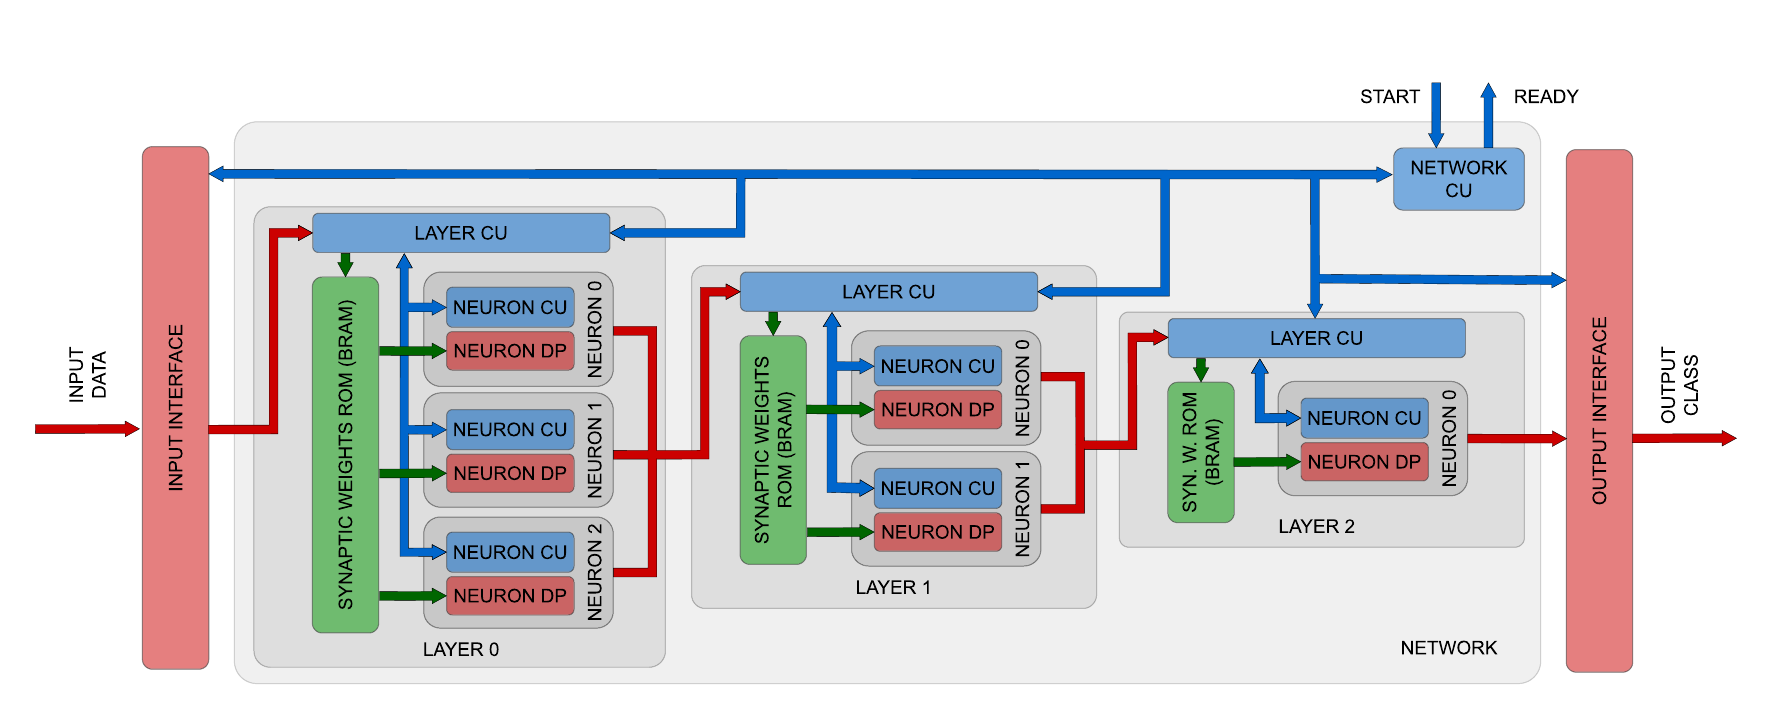
\includegraphics[width=\linewidth]{figures/spikerplus_generated_architecture_original.png}
	\caption{High-level Spiker+ Architecture for a Feed-Forward Fully Connected \gls{snn} \cite{Carpegna2025}}
	\label{fig:spikerplus-generated-architecture}
\end{figure}

\subsection{Architecture Hierarchy and Baseline Instance}

At the accelerator boundary, an input interface converts encoded spike addresses into the internal spike-vector representation expected by the network. In the generated baseline, the \texttt{full\_accelerator} module performs this conversion using a decoder and a bank of input registers. The network output is represented internally as a vector of neuron spikes, while an output multiplexer allows an individual output spike to be selected through the external interface.

The \texttt{network} module instantiates the network controller and the generated layer modules. The Network CU governs the temporal evolution of the \gls{snn} over a configurable number of processing cycles. It distributes a start condition to the layers, waits for their completion signals, and generates a restart signal when the state of the network must be initialized for a new sample.

The baseline instance examined in this work contains 784 external excitatory inputs and a layer of ten output neurons. The output spikes are returned to the same layer as inhibitory inputs, creating recurrent competition between the output neurons. The layer therefore contains separate excitatory and inhibitory input paths, their corresponding weight memories, ten neuron instances, and a barrier that collects the neuron outputs. Although these dimensions are specific to the generated baseline, the same hierarchy is used by Spiker+ for other supported network configurations.

\subsection{Processing and Synchronization}

Spiker+ combines sequential synapse processing with parallel neuron processing. Within a layer, the input controller iterates over the excitatory input addresses and then over the inhibitory inputs. For each address, the corresponding input spike and one weight for every postsynaptic neuron are selected. The ten neurons can consequently process the same presynaptic event in parallel, while the individual presynaptic connections are supplied sequentially. This organization avoids implementing a separate processing datapath for every synapse while retaining parallelism across the neurons of a layer.

Communication between the control levels follows a start/ready handshake. The Network CU starts a network cycle only when the participating layers are ready. At the layer level, the Layer CU initiates the next input operation and waits until the neurons report completion. Their \texttt{neuron\_ready} signals are combined with the barrier status to form the layer-level completion condition. The barrier stores the produced output spikes and prevents the controller from advancing while one or more neuron operations are unfinished.

This synchronization mechanism is directly relevant to online learning. A weight update must remain associated with the input address and postsynaptic neuron that produced the learning decision. The layer must therefore retain the relevant address and state information until the update is complete, and its ready condition must account for any additional learning and write-back latency.

\subsection{Neuron Datapath and Weight Storage}

Each baseline neuron is separated into a finite-state control unit and an arithmetic datapath, as indicated in Figure \ref{fig:spikerplus-generated-architecture}. The controller selects operations for initialization, excitatory integration, inhibitory integration, leakage, firing, and idle behaviour. The datapath stores the membrane potential in a signed register, selects the appropriate update value, performs addition or subtraction, and compares the result with the firing threshold. Leakage is implemented through a shift operation, and firing uses a subtractive reset so that the residual membrane potential is preserved.

In the original neuron interface, the membrane potential remains internal to the datapath. The surrounding layer receives only the output spike and the completion status. This interface is sufficient for inference, but it does not expose the postsynaptic state required by \gls{sdsp}. Integrating the learning rule therefore requires an additional connection between the neuron state and the learning logic without changing the existing inference operations.

The baseline layer stores excitatory and inhibitory weights in separate generated memories. The current input index is used as the read address, and one access returns the weights connected to all ten postsynaptic neurons. This memory organization matches the processing schedule because all neurons operate on the selected presynaptic input in parallel. In the examined design, the membrane potential uses a 16-bit representation and both excitatory and inhibitory weights use three-bit values.

The weight memories are initialized from the parameters produced during offline training. Their generated interfaces contain a clock, a read address, and weight outputs, but no write-enable signal, write data, or runtime update path. The stored values therefore remain constant during inference. This is the principal storage limitation that prevents the baseline accelerator from supporting online learning.

\subsection{Implications for the Learning Extension}

The architecture shown in Figure \ref{fig:spikerplus-generated-architecture} already provides a modular separation between network control, layer control, neuron computation, and synaptic storage. This structure makes it possible to introduce learning without replacing the complete accelerator. Nevertheless, the baseline analysis identifies three required modifications.

First, the postsynaptic membrane potential and the additional activity state required by \gls{sdsp} must be made available outside the original neuron datapath. Second, the static excitatory-weight memory must be replaced or extended with writable storage and a correctly addressed write-back interface. Third, the layer-level control and ready logic must coordinate inference, the learning decision, and completion of the weight update. These requirements guide the architecture developed in the following sections.

\section{Proposed Online-Learning Architecture}
\label{subsec: proposed online learning architecture}

The proposed architecture extends the generated Spiker+ accelerator with a local online-learning path while retaining the original network, layer, and neuron hierarchy. The existing datapath continues to process spikes and update the neuron states, whereas the added path observes the current synaptic and postsynaptic states, evaluates the learning conditions, and writes an updated excitatory weight back to memory. Figure \ref{fig:proposed-online-learning-architecture} presents this relationship at the system level. Blue connections indicate the original inference path, while orange connections show the learning and write-back path introduced in this work.

\begin{figure}[t]
	\centering
	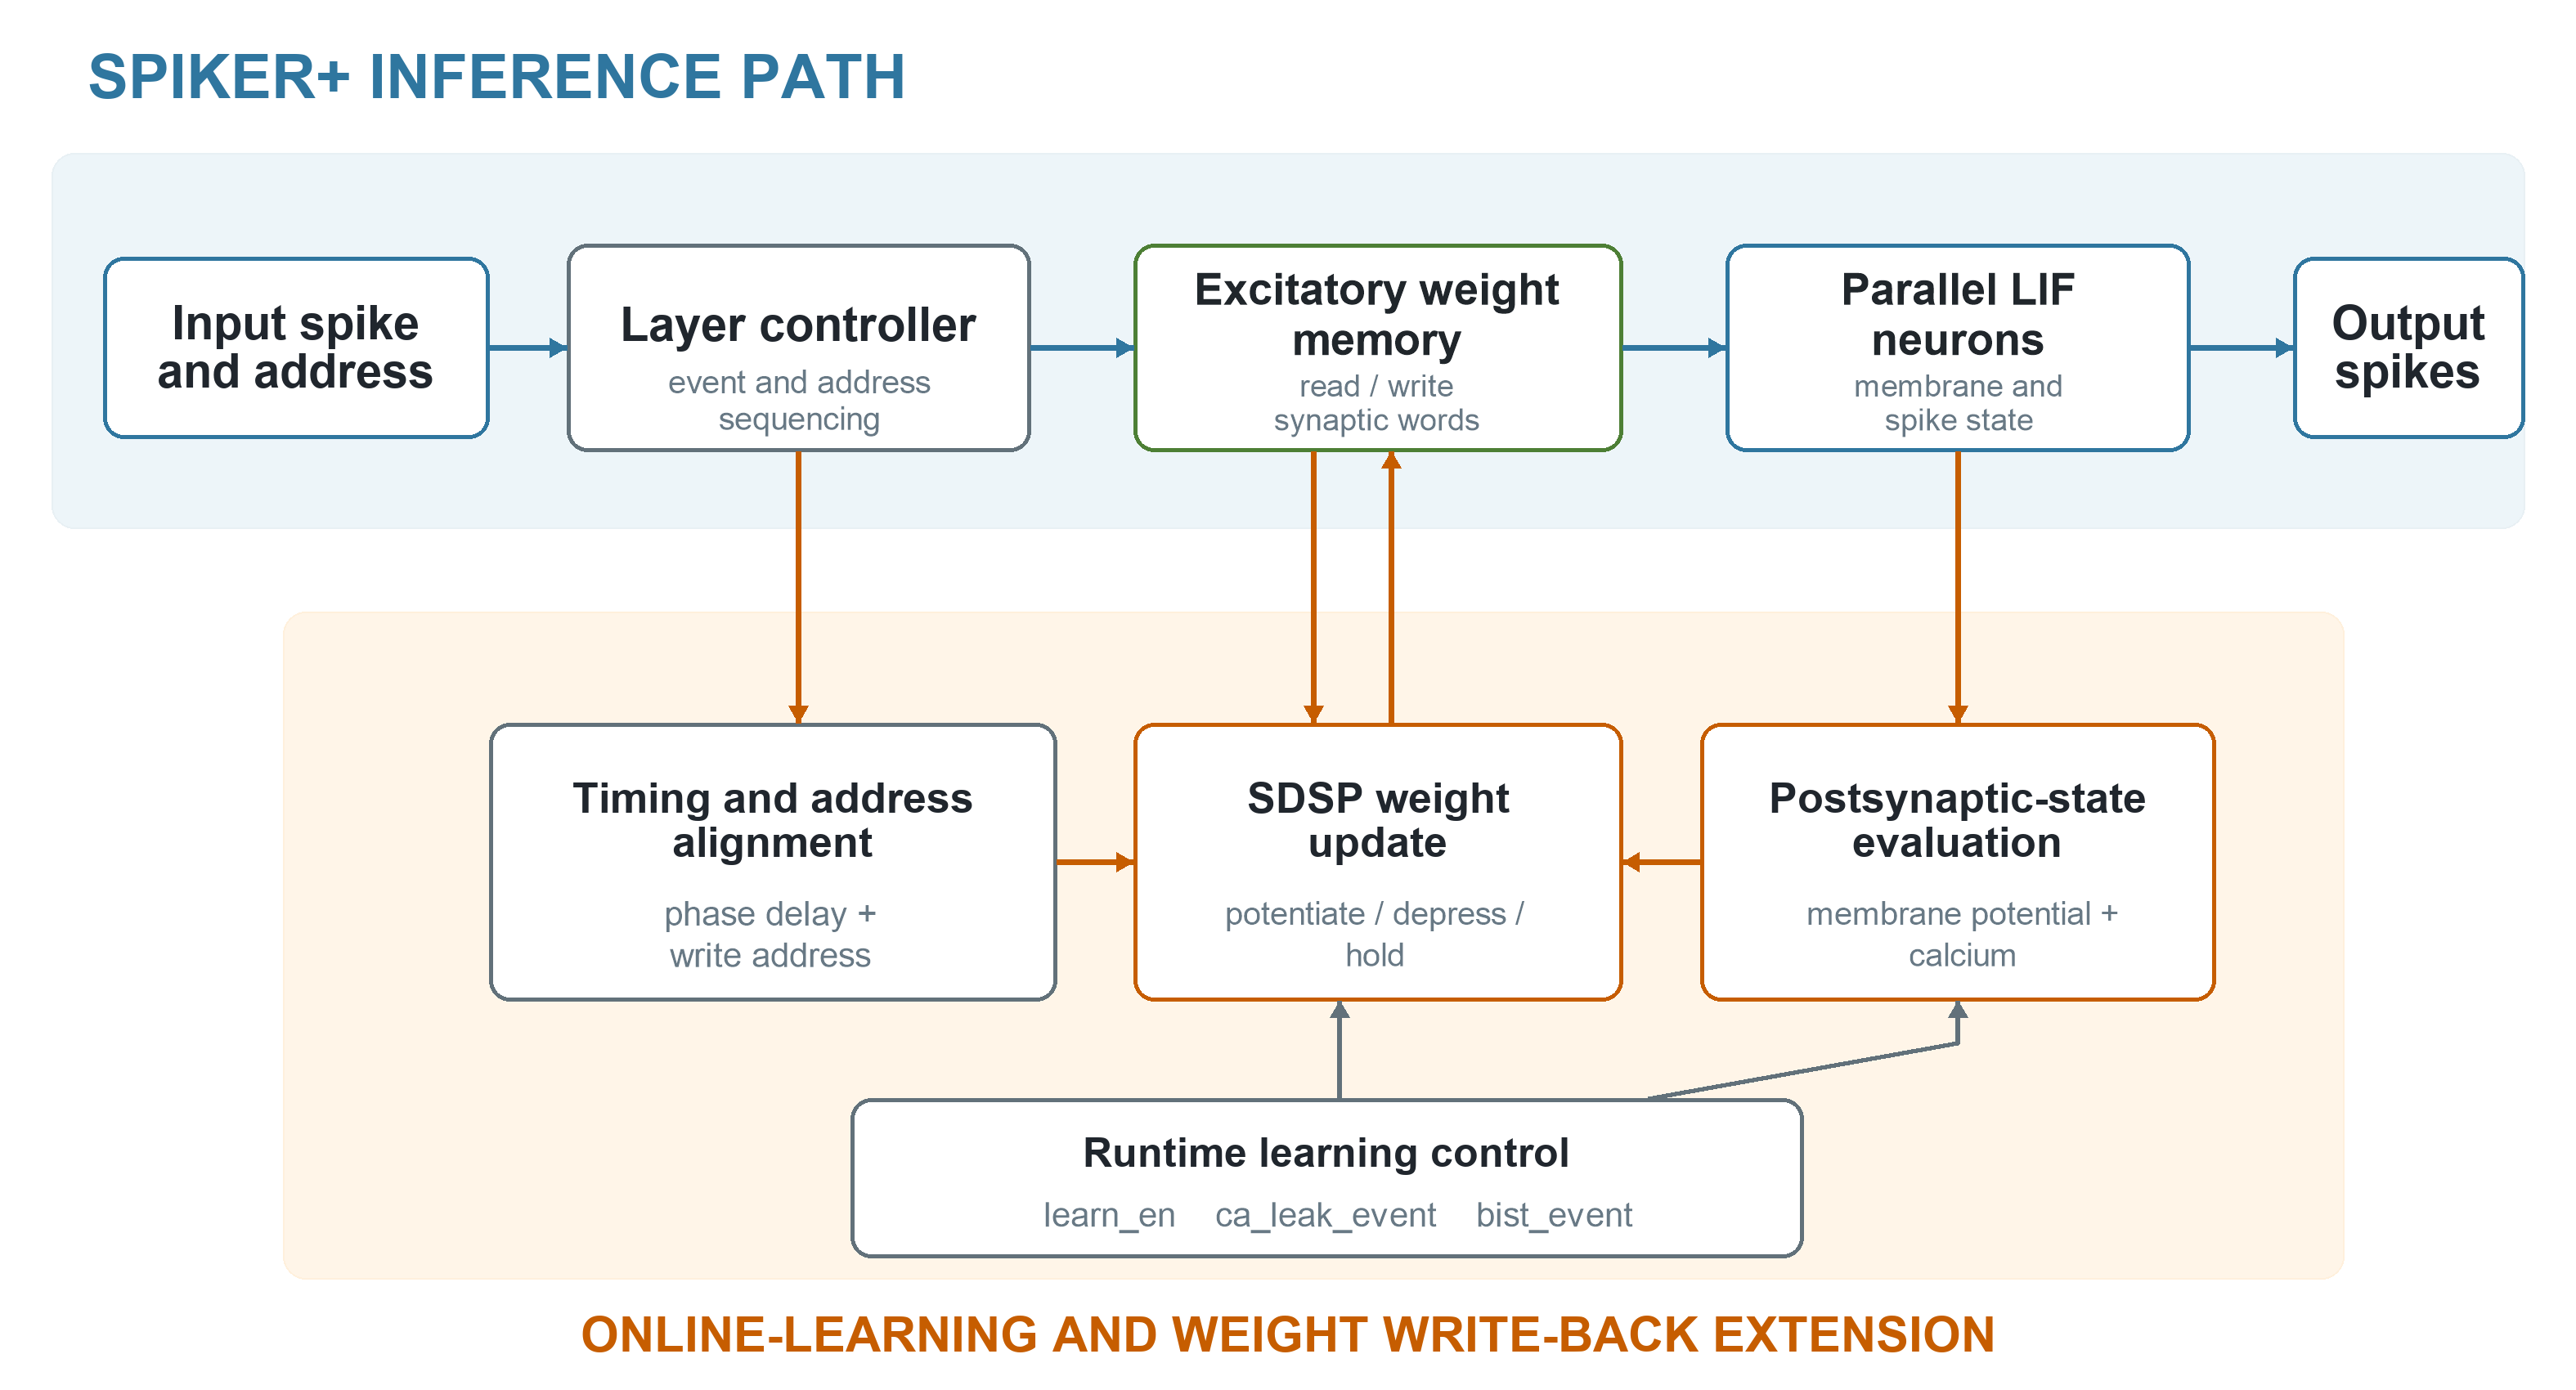
\includegraphics[width=\linewidth]{figures/proposed_online_learning_architecture.png}
	\caption{Integration of the \gls{sdsp} Learning and Weight Write-Back Path into the Spiker+ Architecture}
	\label{fig:proposed-online-learning-architecture}
\end{figure}

\subsection{Overall Organization}

As shown in Figure \ref{fig:proposed-online-learning-architecture}, the network-level controller and the original start/ready coordination remain responsible for executing the generated \gls{snn}. At the layer level, the controller selects a presynaptic address and reads the corresponding synaptic weights. The excitatory weight word is then distributed to the parallel \gls{lif} neuron datapaths, while the fixed inhibitory memory continues to support the recurrent competition between the output neurons. The inference path therefore preserves the processing model of the baseline Spiker+ accelerator \cite{Carpegna2025}.

The principal architectural change is the feedback path from the postsynaptic neurons to the excitatory-weight memory. The modified neuron datapath exposes its membrane potential without changing the existing integration, leakage, firing, or subtractive-reset operations. Each postsynaptic neuron is additionally associated with a calcium counter that represents its recent firing activity. The membrane potential and calcium state are evaluated together to generate the potentiation and depression conditions required by the \gls{sdsp} rule \cite{Brader2007}.

One \gls{sdsp} update unit is instantiated for each postsynaptic neuron. Consequently, all weights contained in the currently read word can be evaluated in parallel, matching the parallel organization of the neuron datapaths. The resulting weight fields are reassembled into an updated word and returned to the excitatory memory. The learning extension is restricted to the feed-forward excitatory synapses; the inhibitory memory and its inference path remain unchanged.

\subsection{Learning and Weight Write-Back Flow}

For every excitatory input transaction, the layer controller supplies a presynaptic event and selects the associated weight word. The same weights are used by the neuron datapaths for synaptic integration and by the learning units as the current synaptic state. In parallel, the learning path receives the postsynaptic membrane potentials, calcium states, and the externally supplied learning-control events. These local quantities determine whether each weight is potentiated, depressed, or retained.

Online learning requires the update to remain associated with the address from which the original weight was read. This is non-trivial because the generated Spiker+ layer prefetches the next weight word while advancing through the presynaptic addresses. The proposed architecture therefore delays the indication of the excitatory processing phase and retains the valid write address. A pending-write signal transfers the update request across the clock boundary so that the completed weight word is written to the correct memory entry. The same mechanism also retains the update belonging to the final excitatory input when the layer controller changes to the next processing phase.

The original read-only excitatory storage is replaced by a writable memory with separate read and write addresses. A read supplies the weights required for the current synaptic operation, while a subsequent write commits the learning result. This organization permits a completed update to be stored while the controller prepares the next input access. Because the entire word is written together, the parallel results produced for all postsynaptic neurons remain synchronized.

During the inhibitory phase, the layer follows the original inference path. Inhibitory weights are read from the unchanged memory and supplied only to the neuron datapaths; no learning request or write-back operation is generated. This separation confines the additional memory and control logic to the synapses that are adapted by the implemented learning rule.

\subsection{Operating Modes and Synchronization}

Three control inputs are added at the accelerator boundary and propagated through the network to the modified layer. The \texttt{learn\_en} signal enables weight updates. When it is disabled, the excitatory-memory write interface remains inactive, the initialized weights are retained, and the accelerator operates in its original inference-only mode. Training and evaluation can therefore be selected at runtime without regenerating the hardware.

The \texttt{ca\_leak\_event} signal controls the decay of the calcium counters independently of the synapse-processing rate. The \texttt{bist\_event} signal activates the bistability mechanism that drives intermediate weights toward stable states. These two events are distributed globally, whereas the membrane potential, calcium state, learning decision, and synaptic weight remain local to the relevant postsynaptic neuron and connection.

The original start/ready synchronization between the network, layer, neurons, and output barrier is retained. The learning request and write-back are aligned with the existing layer schedule by the phase-delay, registered-address, and pending-write logic shown in Figure \ref{fig:proposed-online-learning-architecture}. Therefore, no independent training controller or global learning handshake is required. The modified layer additionally reports when an input event has been accepted and when the corresponding output step is valid, providing precise transaction boundaries for system-level integration and verification.

In summary, the proposed architecture preserves the original event-processing datapath and introduces a local feedback loop for online adaptation. The postsynaptic state determines the learning condition, the presynaptic event identifies the active synaptic word, and the aligned write-back path stores the updated result at the correct address. The next section describes the digital realization of the \gls{sdsp} update function used inside this architecture.

\section{Digital Realization of the SDSP Learning Rule}
\label{subsec: digital sdsp realization}

The digital learning path follows the hardware-oriented organization used in ODIN: the postsynaptic state is evaluated separately from the synaptic weight update, and the resulting direction information is supplied to a compact arithmetic datapath \cite{Frenkel2019ODIN}. The proposed design applies this separation to every postsynaptic neuron while retaining the parallel weight organization of the generated Spiker+ layer.

\subsection{Learning Conditions and Compact Update Flow}

Each postsynaptic neuron is associated with a calcium counter that represents its recent firing activity. A postsynaptic spike increments the counter, whereas \texttt{ca\_leak\_event} decrements it. The counter saturates at its upper and lower limits, holds its value when neither operation is requested, and is cleared at the beginning of a new sample. This follows the interpretation of the calcium state used in the digital \gls{sdsp} implementation of ODIN \cite{Frenkel2019ODIN}.

At the arrival time \(t_{\mathrm{pre}}\) of a presynaptic spike, the current calcium state and membrane potential determine the direction of the possible weight change. The two update cases are expressed as

\begin{equation}
\begin{cases}
w \rightarrow w+1, &
V_{\mathrm{mem}}(t_{\mathrm{pre}}) \geq V_{\mathrm{th}},
\quad \theta_1 \leq C(t_{\mathrm{pre}}) < \theta_3\\
w \rightarrow w-1, &
V_{\mathrm{mem}}(t_{\mathrm{pre}}) < V_{\mathrm{th}},
\quad \theta_1 \leq C(t_{\mathrm{pre}}) < \theta_2
\end{cases}
\label{eq:sdsp-weight-update-conditions}
\end{equation}

Figure \ref{fig:sdsp-weight-update-overview} shows the inputs and outputs of the \gls{sdsp} online-learning module. The comparator evaluates the conditions in Equation \ref{eq:sdsp-weight-update-conditions} and exposes them through the Boolean signals \texttt{up} and \texttt{down}. When \texttt{spk\_pre} is asserted, the update datapath samples these conditions and either increments, decrements, or retains the current weight. If no presynaptic spike is active, the separate \texttt{bistability} input can request an update based on the most significant bit of the current weight. Separating the condition state from the update trigger allows the arithmetic datapath to read only the decision required at the event time. The detailed arithmetic implementation is described in the next subsection.

\begin{figure}[t]
	\centering
	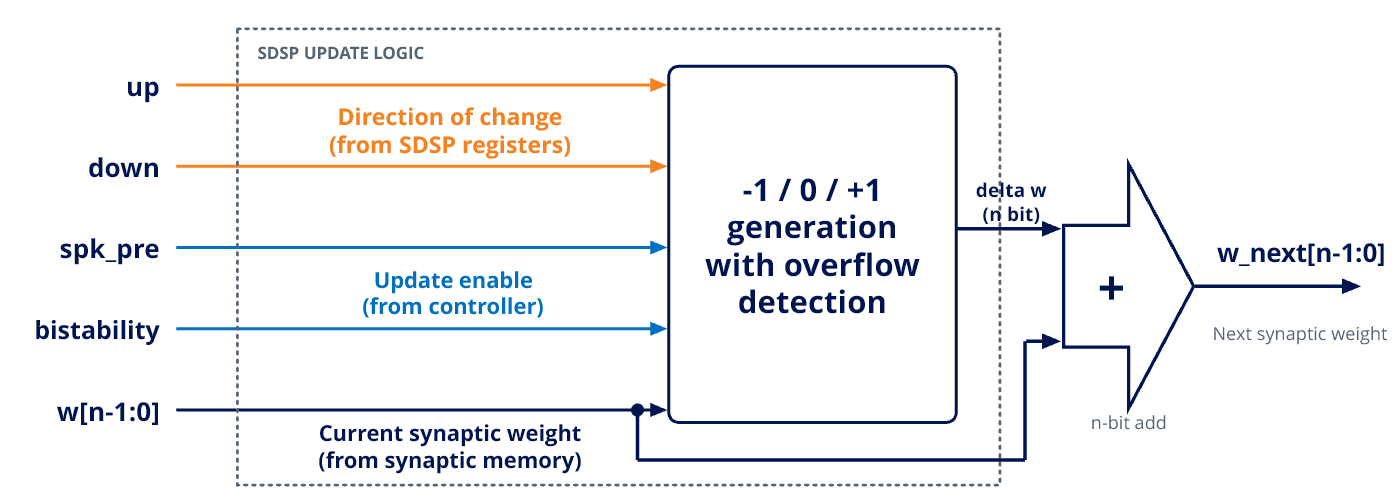
\includegraphics[width=\linewidth]{figures/sdsp_weight_update_overview.png}
	\caption{Control and Arithmetic Organization of the \gls{sdsp} Weight-Update Datapath}
	\label{fig:sdsp-weight-update-overview}
\end{figure}

This organization keeps the learning decision simple. The neuron-side state determines only the direction of change, while the synaptic datapath performs the bounded arithmetic update. It also matches the memory organization of the modified Spiker+ layer: all weights belonging to the selected presynaptic address are read together, and one update datapath evaluates each postsynaptic weight in parallel.

\subsection{Detailed Weight-Update Datapath}

Figure \ref{fig:sdsp-weight-update-datapath} shows the detailed structure of \texttt{sdsp\_top}. The \texttt{delta\_w\_generator} receives \texttt{up}, \texttt{down}, \texttt{spk\_pre}, \texttt{bist}, and the most significant bit of the current weight. It converts the requested operation into the \texttt{delta\_w} word and the carry input \texttt{cin} used by the \(N\)-bit adder.

The generator does not produce a signed arithmetic value such as \(-1\) directly. Instead, addition and subtraction are represented through an \(N\)-bit two's-complement encoding and the carry input of the adder. For an increment, \texttt{delta\_w} is set to all zeros and \texttt{cin} is asserted, so that the adder evaluates \(w_{\mathrm{current}}+0+1\). For a decrement, \texttt{delta\_w} is set to all ones and \texttt{cin} is cleared. The all-one word represents \(2^N-1\), which is equivalent to \(-1\) modulo \(2^N\), and the same unsigned adder therefore evaluates \(w_{\mathrm{current}}-1\). When no update is requested, both outputs are zero and the current weight is passed through unchanged. This encoding explains why both \texttt{delta\_w} and \texttt{cin} are supplied by the generator to the adder: together they express the complete update operation without requiring a separate subtractor or a signed datapath.

\begin{figure}[t]
	\centering
	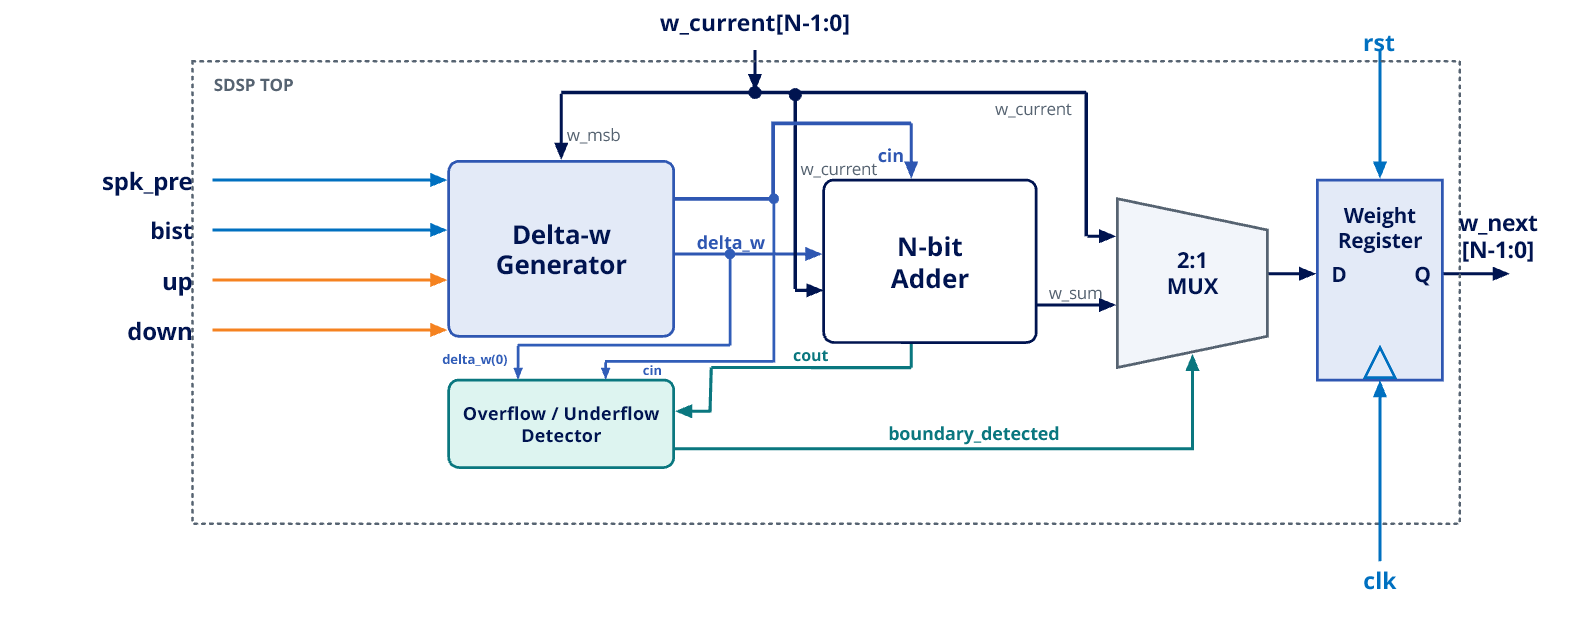
\includegraphics[width=\linewidth]{figures/sdsp_digital_datapath.png}
	\caption{\gls{rtl} Datapath for Bounded \gls{sdsp} Weight Increment and Decrement}
	\label{fig:sdsp-weight-update-datapath}
\end{figure}

For spike-driven learning, \texttt{spk\_pre} has priority and the generator uses the current \texttt{up}/\texttt{down} state. When no presynaptic spike is active, \texttt{bist} can apply the bistability mechanism described for ODIN \cite{Frenkel2019ODIN}. The most significant weight bit identifies the lower or upper half of the numerical range. A bistability event then moves an intermediate weight toward the corresponding low or high stable region.

The adder combines the encoded change with \texttt{w\_current} and produces \texttt{w\_sum} together with the carry output \texttt{cout}. The overflow/underflow detector evaluates \texttt{delta\_w(0)}, \texttt{cin}, and \texttt{cout}. The solid junctions in Figure \ref{fig:sdsp-weight-update-datapath} indicate that the detector inputs branch from the same \texttt{delta\_w} and \texttt{cin} signals used by the adder. If an increment at the maximum value or a decrement at zero would wrap the unsigned weight, \texttt{boundary\_detected} makes the multiplexer retain \texttt{w\_current}. Otherwise, the multiplexer forwards \texttt{w\_sum}. The weight register captures the selected value on the active clock edge and is reset through \texttt{rst}.

One \gls{sdsp} datapath is instantiated for each postsynaptic neuron, and the resulting fields are combined into the complete word written back to the excitatory memory. The arithmetic update therefore remains local, while the address-alignment logic described in Section \ref{subsec: proposed online learning architecture} preserves the association between the updated word and the correct presynaptic input.

\section{Integration into the Spiker+ Accelerator}
\label{subsec:integration-into-spikerplus}

The learning extension is integrated at the layer level because this is the lowest level of the Spiker+ hierarchy at which the presynaptic address, the synaptic weight word, and all postsynaptic neuron states are available together. The network-level scheduler and the original neuron-control sequence are retained \cite{Carpegna2025}. The modified layer adds only the state-observation, update, and memory-write functions required for online learning.

\begin{figure}[t]
	\centering
	\makebox[\linewidth][c]{%
		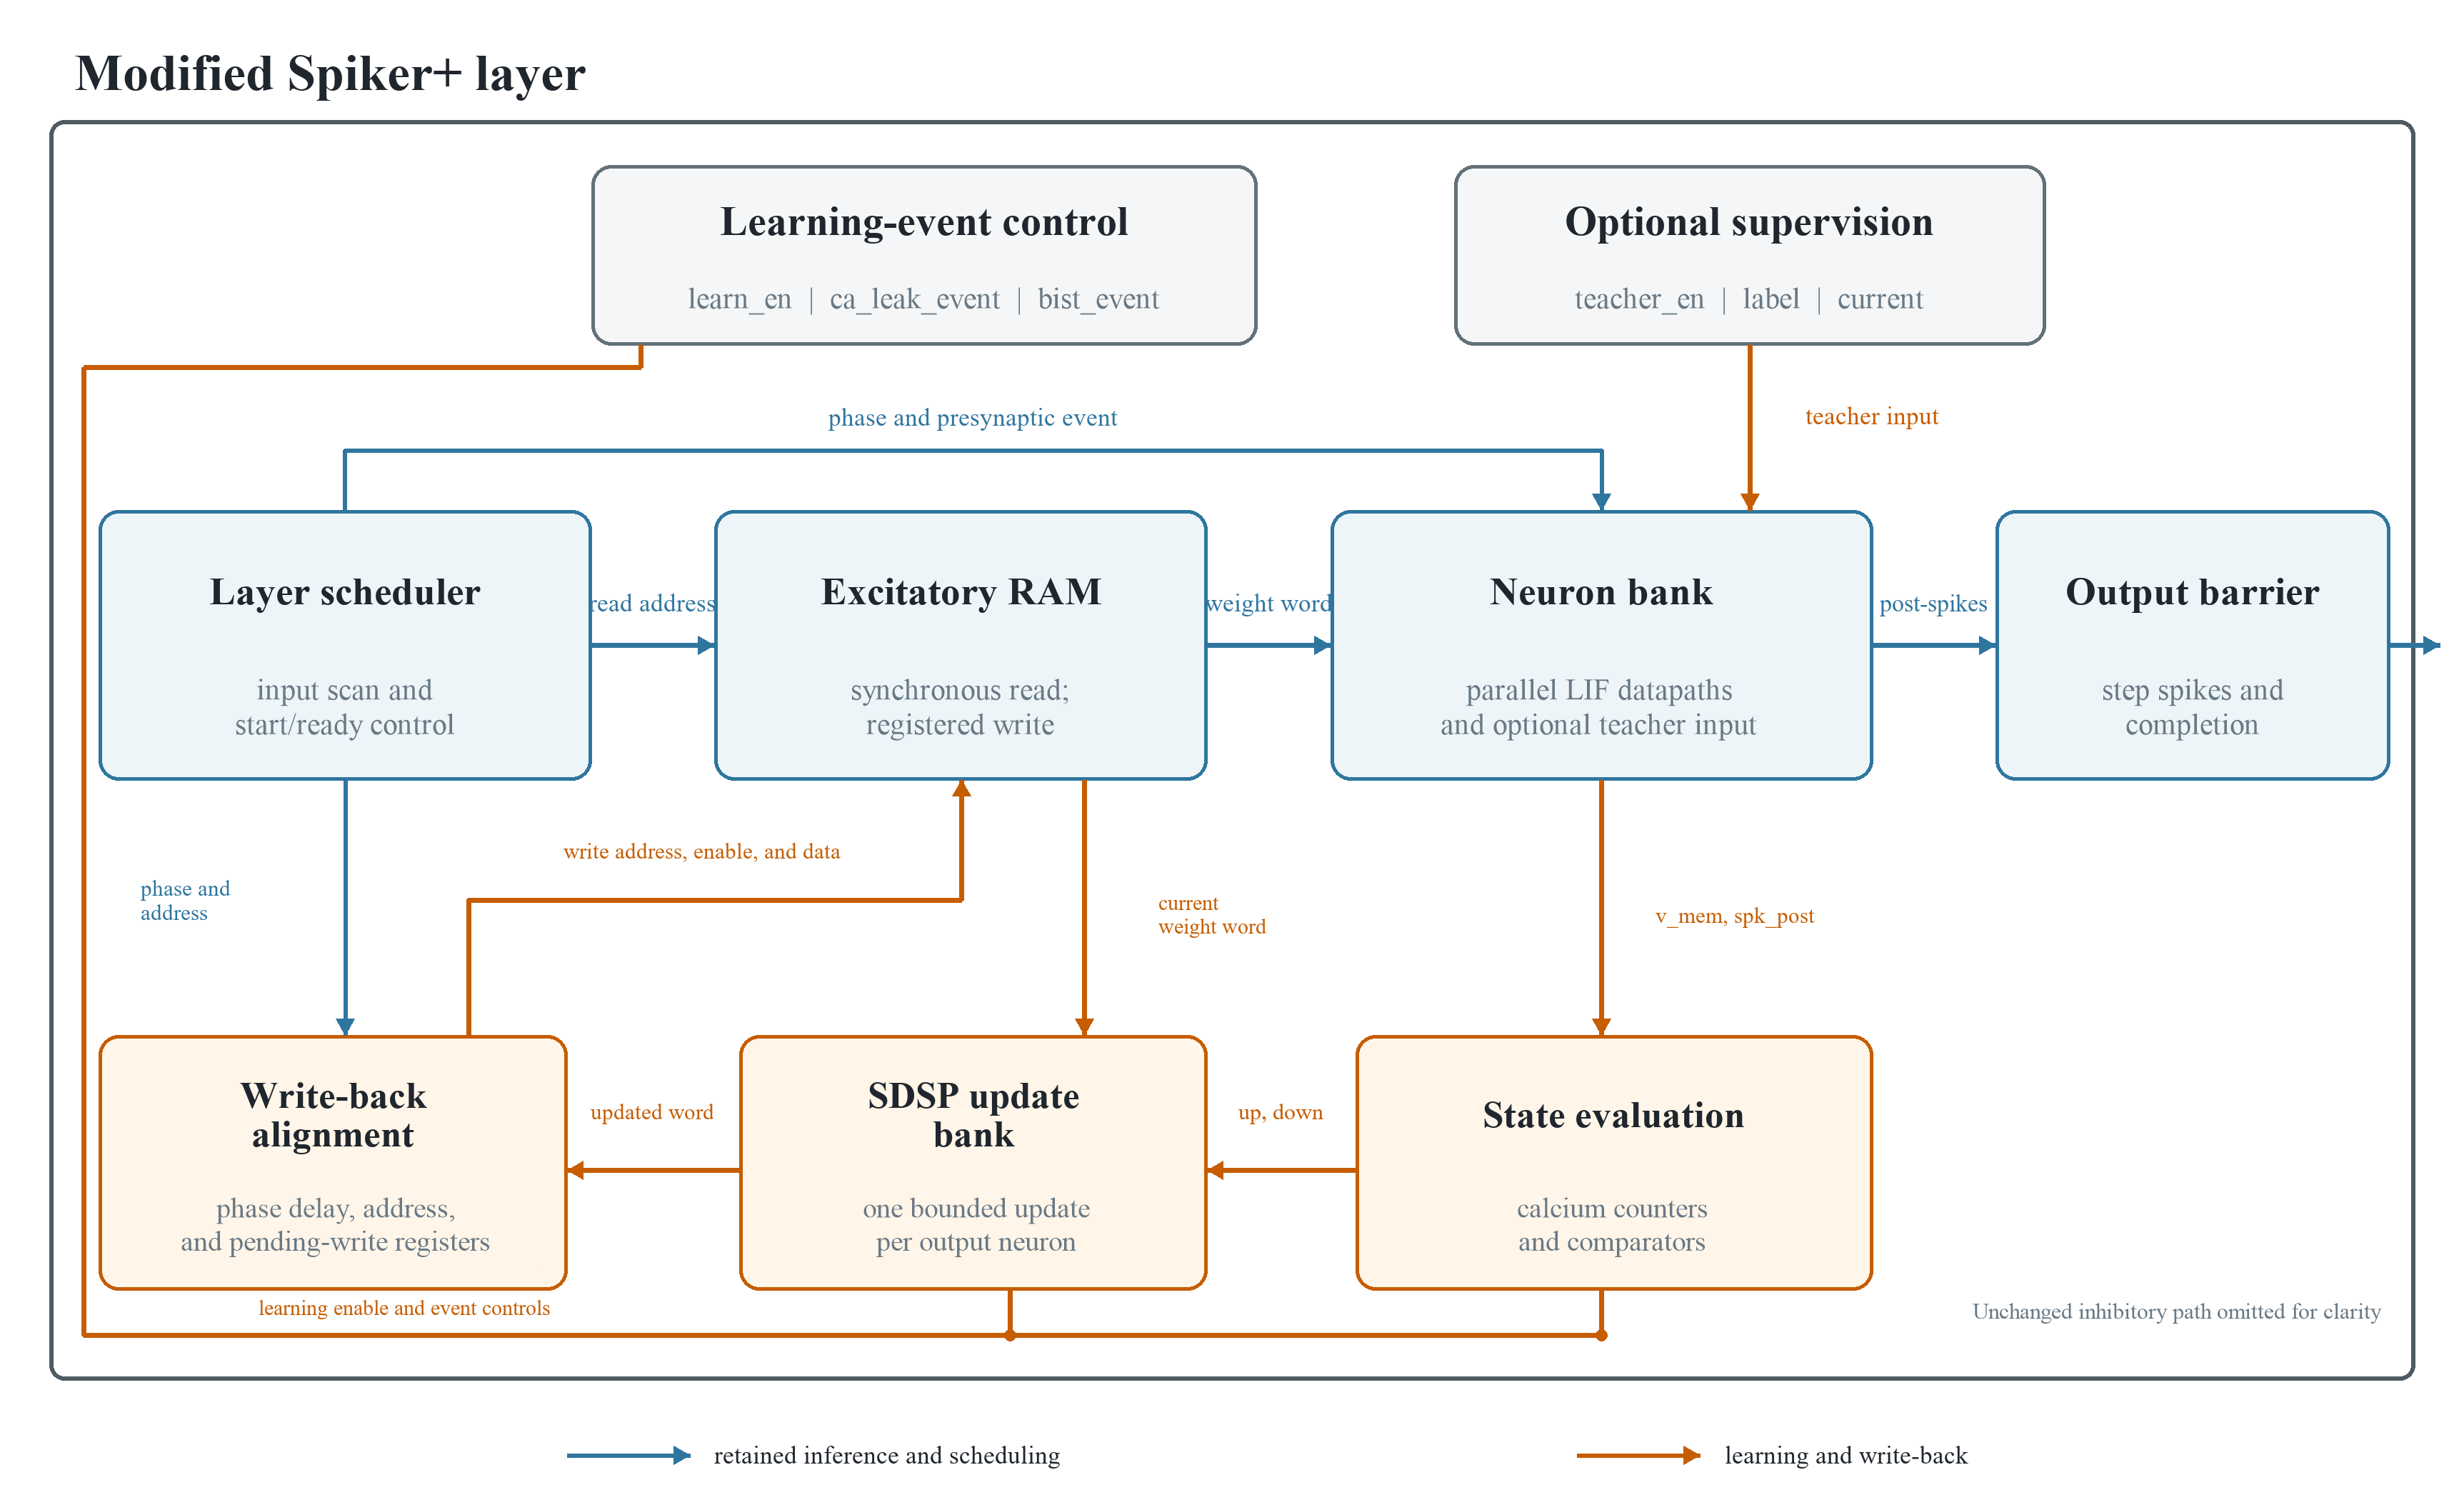
\includegraphics[width=1.06\linewidth]{figures/spiker_sdsp_layer_integration.png}%
	}
	\caption{Layer-Level Integration of the \gls{sdsp} State-Evaluation and Weight Write-Back Paths into Spiker+}
	\label{fig:spiker-sdsp-layer-integration}
\end{figure}

\subsection{Layer-Level Integration and State Formation}

Figure \ref{fig:spiker-sdsp-layer-integration} separates the retained inference path from the added learning feedback path. The layer scheduler continues to scan the excitatory inputs sequentially and supplies the active phase, presynaptic event, and read address. One word from the excitatory memory contains the weights from the selected input to all output neurons. The complete word is therefore delivered to the parallel neuron bank in one access, preserving the processing organization of the generated accelerator. The output barrier and the recurrent inhibitory path are unchanged; the latter is omitted from the figure because it is not modified by the learning extension.

For each output neuron, the current weight is used simultaneously by the neuron datapath and by one \gls{sdsp} update unit. The modified neuron interface exposes the membrane potential and postsynaptic spike. A local calcium counter and comparator convert these quantities into the two update conditions described in Section \ref{subsec: digital sdsp realization}. The same structure is replicated for every output neuron, so all fields in the selected weight word are evaluated in parallel and reassembled into one updated word.

The learning-event interface supplies the global enable, calcium-decay event, and bistability event shown at the top of Figure \ref{fig:spiker-sdsp-layer-integration}. These controls determine when local state is updated and when a weight modification may be committed; they do not replace the normal layer schedule. The final implementation also includes an optional supervision path. At the beginning of each network time step, the configured teacher current is applied only to the output neuron selected by the class label, and only when both supervision and learning are enabled. This current changes the target neuron's membrane state and therefore influences the subsequent local \gls{sdsp} decision. It does not write a weight directly, so weight modification remains governed by the same presynaptic event and postsynaptic-state conditions as the unsupervised path.

\subsection{Address-Aligned Read--Modify--Write Sequence}

Replacing the excitatory read-only storage with writable memory creates a timing problem: the Spiker+ input scanner advances while the synchronous memory prefetches the next weight word. The learning result must nevertheless be written to the address from which its original weight was obtained. Figure \ref{fig:spiker-sdsp-writeback-sequence} summarizes the resulting sequence for an arbitrary excitatory address \(k\).

\begin{figure}[t]
	\centering
	\makebox[\linewidth][c]{%
		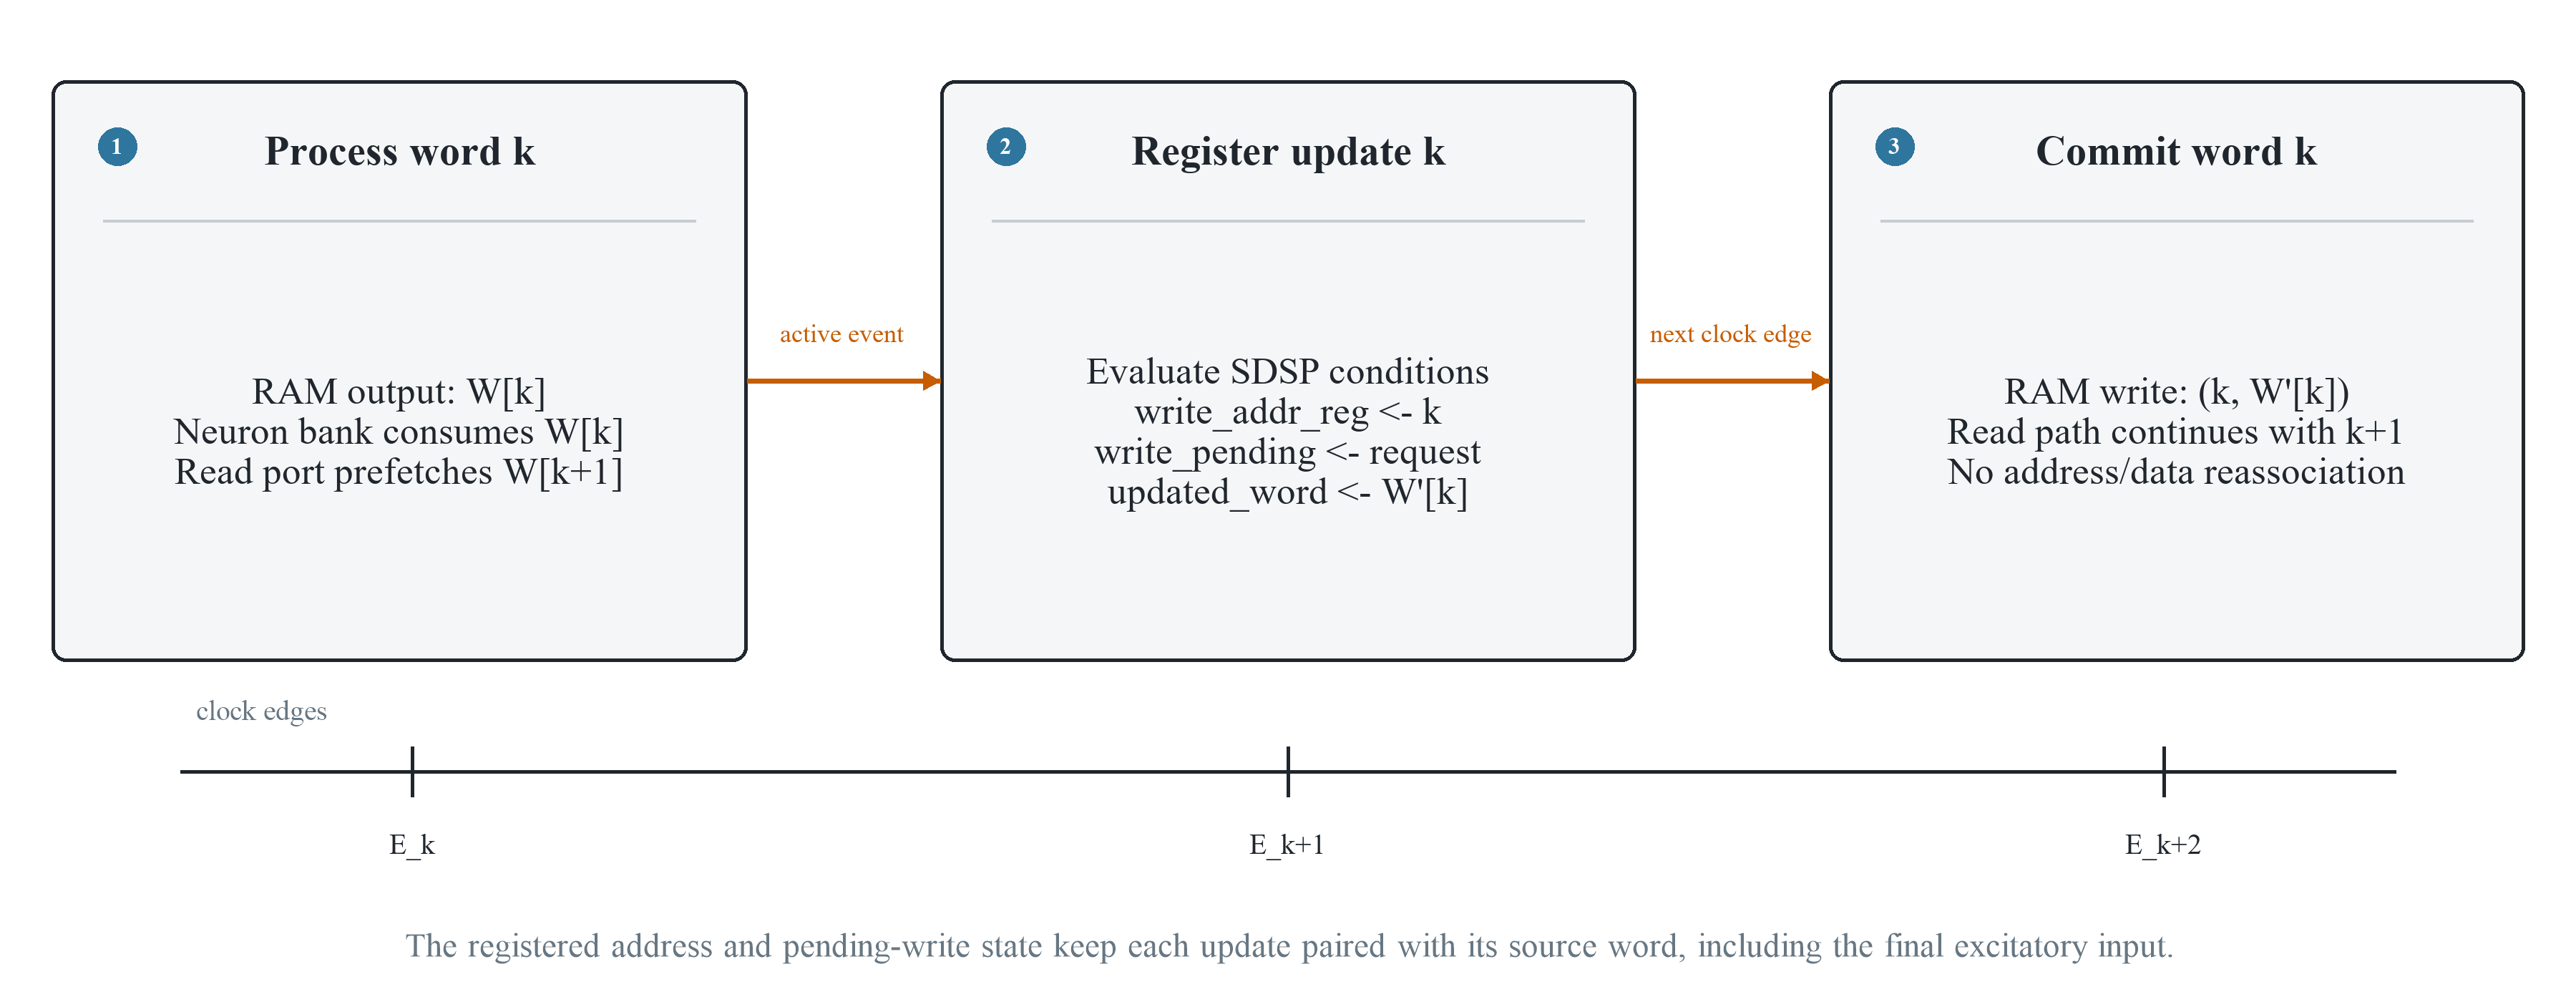
\includegraphics[width=1.05\linewidth]{figures/spiker_sdsp_writeback_sequence.png}%
	}
	\caption{Registered Read--Modify--Write Sequence for an Excitatory Weight Word}
	\label{fig:spiker-sdsp-writeback-sequence}
\end{figure}

While the neuron bank consumes word \(W[k]\), the address converter already requests the next word from the synchronous read port. A learning request is generated only when learning is enabled, the delayed excitatory phase is active, the current address is valid, and either a presynaptic spike or a bistability event requests an update. The delayed phase is important at the end of the scan: it represents the operation associated with the already-prefetched word even when the layer controller begins to leave the excitatory phase.

When the request is active, the current counter value is captured in the write-address register and the request is transferred to the pending-write register. In parallel, the ten \gls{sdsp} units produce the updated word \(W'[k]\). On the following write opportunity, the registered address, pending state, and updated word drive the memory write port together. Registering the address and request therefore prevents the prefetched word for address \(k+1\) from being associated with the update generated for address \(k\). The same mechanism preserves the update for the final excitatory input before the controller proceeds to inhibitory processing.

The excitatory memory uses one synchronous read port and one write port with read-first behaviour. A completed update can consequently be written while the read pipeline advances to the next input. The full word is committed in one operation, so the parallel per-neuron update results remain aligned. The inhibitory weights remain in the original read-only path because they are not adapted by the implemented learning rule.

\subsection{Inference Compatibility and Integration Boundary}

When learning is disabled, no new write request is produced. After an already pending operation has completed, the write port remains inactive and the initialized weights are retained. The layer therefore follows the blue inference path in Figure \ref{fig:spiker-sdsp-layer-integration}, including the existing start, restart, completion, neuron, and output-barrier coordination. Enabling learning activates the orange feedback path without introducing a second layer scheduler or a separate global training handshake.

The integration boundary of this chapter ends at the accelerator interfaces. Processor communication, external-memory transfers, bus protocols, and board-specific IP determine how spike frames and control values reach the accelerator, but they do not change the layer-internal learning sequence. These platform-specific elements are therefore described separately in Chapter \ref{sec:implementation}.

\section{Assessment of Dynamic Partial Reconfiguration Applicability}
\label{subsec:dpr-applicability}

\Gls{dpr} was considered during the initial design phase as a possible means of exchanging online-learning functionality at runtime. As introduced in Section \ref{subsec: dynamic partial reconfiguration}, this approach requires every \gls{rm} assigned to the same reconfigurable partition to use an identical boundary with the static design \cite{UG909}. A useful application would therefore require at least two learning modules that are both needed at runtime and can operate through a common interface without changing the surrounding accelerator.

This condition is not satisfied by the present learning architecture. The implemented \gls{sdsp} unit is tightly coupled to the neuron and layer datapaths through the algorithm-specific signals \texttt{up}, \texttt{down}, \texttt{bist\_event}, \texttt{exc\_spike}, \texttt{learning\_request}, \texttt{w\_current}, and \texttt{w\_next}. Its operation also depends on the calcium counters, comparator outputs, weight-memory organization, and the address-aligned read--modify--write schedule described in the preceding sections. These connections form a specialized \gls{sdsp} interface rather than a generic boundary for interchangeable learning rules.

Other online-learning algorithms would generally require different state variables, event histories, update timing, weight representations, or supervision signals. They could not be placed in the same reconfigurable partition without first introducing a common learning-module abstraction and additional adapters in the static region. Such an abstraction would either constrain the alternative modules to the \gls{sdsp} interface or move a substantial part of their algorithm-specific logic into the static design. In both cases, the intended flexibility of runtime reconfiguration would be substantially reduced.

State continuity introduces a further difficulty. The learning process depends on persistent neuron and synapse state, including calcium activity and the current weight memory. If only the update function were reconfigured, algorithm-specific state would remain distributed throughout the static design. If the state-holding logic were included in the reconfigurable partition, changing the module would require an additional mechanism for state preservation, translation, and restoration. This would increase the implementation and verification effort without providing a corresponding benefit for the single \gls{sdsp} learning rule evaluated in this work.

Implementing \gls{dpr} would additionally require partition floorplanning, partial-bitstream generation, interface isolation, reconfiguration control, and verification of every supported module combination. The target system has no operational requirement to switch learning algorithms while processing an input sequence, and no second interface-compatible learning module is part of the intended design. \gls{dpr} would therefore add architectural and tool-flow complexity without improving the functionality, performance, or experimental value of the accelerator.

Based on these considerations, the final implementation uses a static \gls{fpga} configuration, and \gls{dpr} is excluded from the scope of implementation and evaluation. This is a deliberate design decision: the contribution of this thesis lies in the integration and hardware realization of \gls{sdsp}-based online learning within Spiker+, together with its system-level deployment. \Gls{dpr} would become meaningful only if future work defined a generic learning interface and provided multiple compatible learning modules for an explicit runtime-switching use case.

% !TEX root = thesis.tex
\chapter{Implementation}
\label{sec:implementation}

This chapter describes the realization of the architecture developed in Chapter \ref{sec:design_methodology} as a synthesizable and board-deployable system. The proposed \gls{sdsp} learning path is integrated with the generated Spiker+ accelerator, while the surrounding system provides the control, data-transfer, and memory-access mechanisms required to operate the accelerator on an embedded \gls{fpga} platform. The implementation therefore covers both the modified neural-network hardware and its connection to the processor-side software environment.

The chapter first introduces the target platform and the PYNQ overlay abstraction. The subsequent sections describe the realization of the learning-related \gls{rtl} modules, their integration into the Spiker+ hierarchy, and the board-level communication path used to transfer spike data and control the accelerator. Verification and implementation results are presented separately in Chapter \ref{sec:results_and_evaluation}.

\section{Target Platform and PYNQ Overlay}
\label{subsec:target-platform-and-overlay}

The implementation targets the Digilent PYNQ-Z1 development board. The board combines an embedded processor and reconfigurable logic in a single Zynq-7000 device and is supported by the PYNQ software environment. This combination is suitable for the present work because processor-side preparation and control can be separated from the latency-sensitive spike processing and online weight updates implemented in hardware.

\subsection{PYNQ-Z1 Hardware Platform}

Figure \ref{fig:pynq-z1-board} shows the PYNQ-Z1 board used for deployment. Its central device is the XC7Z020-1CLG400C Zynq-7000 All Programmable \gls{soc}. The device consists of a \gls{ps}, containing a dual-core ARM Cortex-A9 processor and the fixed memory and peripheral controllers, and a \gls{pl}, which contains the configurable logic resources used for the \gls{snn} accelerator \cite{DigilentPYNQZ1Manual}.

\begin{figure}[t]
	\centering
	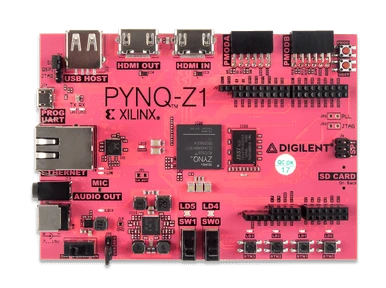
\includegraphics[width=0.78\linewidth]{figures/pynq_z1_board_official.png}
	\caption{Digilent PYNQ-Z1 Development Board \cite{DigilentPYNQZ1Product}}
	\label{fig:pynq-z1-board}
\end{figure}

Table \ref{tab:pynq-z1-resources} summarizes the platform resources most relevant to this implementation. The 512~MB external \gls{ddr} \gls{sdram} provides storage for input spike sequences and processor-side data, while the configurable logic implements the accelerator and its interface logic. The available logic slices and \gls{bram} resources are particularly relevant to the parallel neuron datapaths and writable synaptic-weight memories. Although the board also provides video, audio, Ethernet, USB, Pmod, and Arduino-compatible interfaces, these peripherals are not required by the implemented accelerator and are therefore not considered further.

\begin{table}[htbp]
	\centering
	\caption{PYNQ-Z1 Resources Relevant to the Implemented System \cite{DigilentPYNQZ1Manual}}
	\label{tab:pynq-z1-resources}
	\begin{tabularx}{0.92\linewidth}{@{}lX@{}}
		\toprule
		\textbf{Resource} & \textbf{Platform characteristic} \\
		\midrule
		Zynq device & XC7Z020-1CLG400C \\
		Processing system & Dual-core ARM Cortex-A9, up to 650\,MHz \\
		Programmable logic & 13,300 logic slices and 220 DSP slices \\
		On-chip memory & 630~KB of block RAM \\
		External memory & 512~MB DDR3 with a 16-bit data bus \\
		Boot and storage & 16~MB QSPI flash and microSD interface \\
		\bottomrule
	\end{tabularx}
\end{table}

The functional relationship between the two parts of the Zynq device is illustrated in Figure \ref{fig:pynq-overlay-concept}. The \gls{ps} executes the PYNQ software stack and accesses the external DDR memory, whereas custom peripherals and accelerators are instantiated in the \gls{pl}. Standard AXI connections provide control and data exchange between the two domains. In the implemented system, a general-purpose AXI master port is used for accelerator control, a high-performance AXI slave port gives the \gls{dma} engine access to DDR, and a 100\,MHz fabric clock drives the accelerator and its interface logic. Completion and error events can be returned to the processor through fabric interrupts.

\begin{figure}[t]
	\centering
	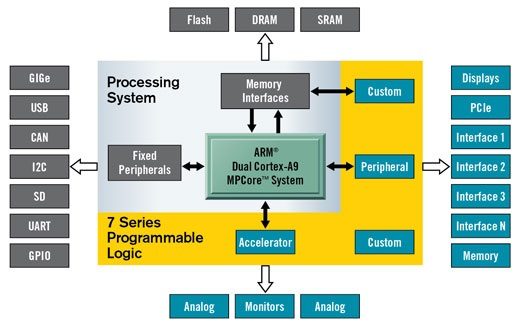
\includegraphics[width=0.78\linewidth]{figures/pynq_overlay_concept_official.png}
	\caption{Processing-System and Programmable-Logic Organization of the Zynq-7000 \gls{soc} \cite{PYNQOverlays}}
	\label{fig:pynq-overlay-concept}
\end{figure}

This heterogeneous organization assigns tasks according to their computational characteristics. The processor handles configuration, memory management, and test coordination, while the \gls{pl} performs deterministic spike processing and local synaptic updates. The external DDR memory is therefore used as the exchange point for input data rather than as storage for individual synaptic updates; the latter remain inside the accelerator's writable weight memories.

\subsection{PYNQ Overlay Abstraction}

PYNQ represents a hardware design as an \emph{overlay}: a configurable hardware system that can be loaded into the \gls{pl} and controlled from Python running on the \gls{ps}. A typical overlay is distributed with a bitstream file (\texttt{.bit}) and a hardware handoff file (\texttt{.hwh}). The bitstream configures the programmable logic, while the hardware description provides the address map, instantiated \gls{ip} blocks, clocks, and interrupt connections required by the PYNQ software interface \cite{PYNQOverlayLoading,PYNQOverlayDesign}.

For this work, the overlay forms the deployment container around the Spiker+-\gls{sdsp} accelerator. It includes the Zynq processing system, the DDR-facing \gls{dma} path, the AXI control interconnect, buffering for the input stream, and the accelerator wrapper. From the processor side, the software loads the overlay, allocates the input buffers in DDR, configures the accelerator through memory-mapped control registers, starts the data transfer, and reads the produced status and classification results. The learning computation itself remains entirely in the \gls{pl}; the Python environment is used to operate and evaluate the hardware rather than to calculate weight updates.

Loading the overlay configures the complete \gls{pl} design. In this thesis, it is not used to exchange learning modules during execution and should therefore not be confused with the \gls{dpr} approach discussed in Section \ref{subsec:dpr-applicability}. The overlay provides a convenient software-visible boundary for the statically implemented system, whereas the internal \gls{snn} and \gls{sdsp} architecture remains fixed for the duration of an experiment.

\section{RTL Architecture and Module Hierarchy}
\label{subsec:rtl-architecture}

The final Vivado implementation is organized in three nested levels. The generated top-level wrapper contains the complete block design, the block design instantiates the packaged SNN--SDSP accelerator as a custom \gls{ip} core, and the custom IP contains the AXI wrapper together with the complete Spiker+ network and learning hierarchy. This organization keeps the board-specific processing-system and data-movement infrastructure outside the reusable accelerator IP while allowing the complete design to be synthesized through one generated top-level entity. Figure \ref{fig:rtl-hierarchy} shows this final elaborated hierarchy.

\begin{figure}[t]
	\centering
	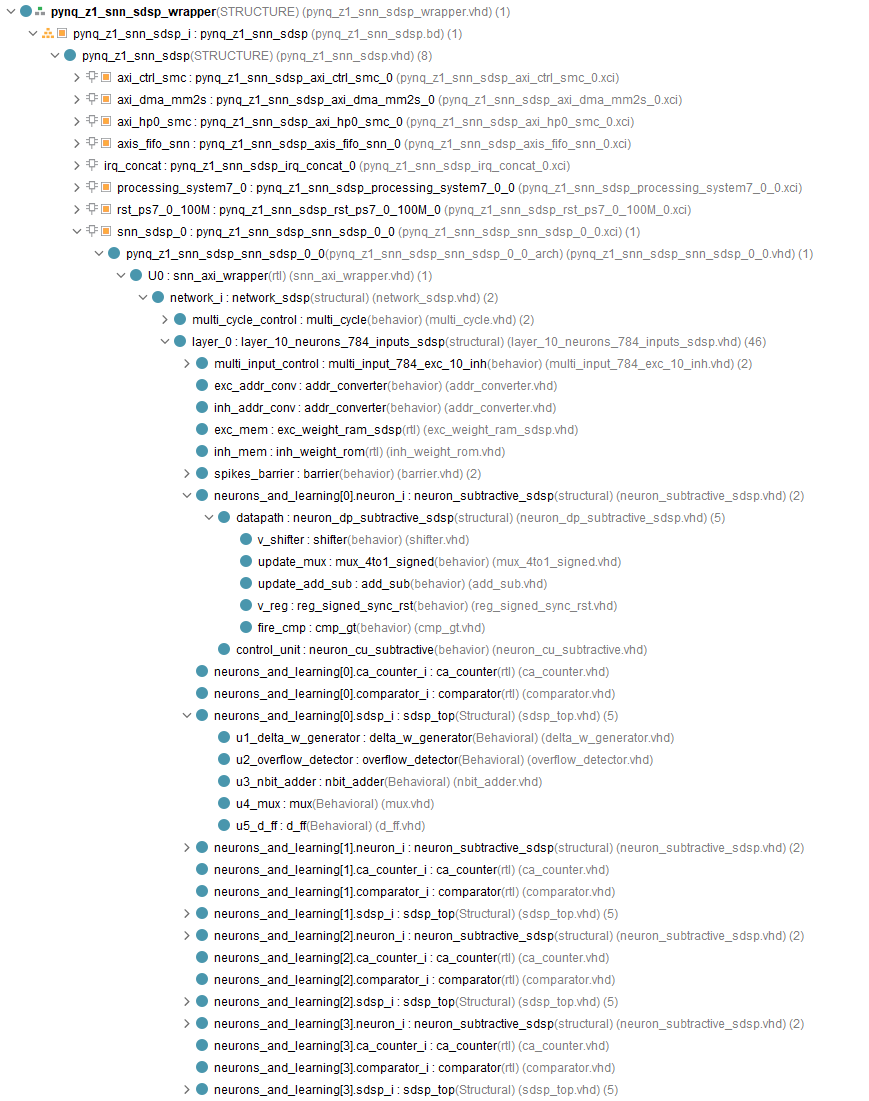
\includegraphics[width=0.92\linewidth]{figures/rtl_hierarchy.png}
	\caption{Final Elaborated \gls{rtl} Hierarchy of the PYNQ-Z1 \gls{snn}--\gls{sdsp} System}
	\label{fig:rtl-hierarchy}
\end{figure}

At the root of the hierarchy, the Vivado-generated entity \texttt{pynq\_z1\_snn\_sdsp\_wrapper} instantiates the block design as \texttt{pynq\_z1\_snn\_sdsp\_i}. Only the DDR and fixed \gls{ps} pins are exposed at this level. The expanded block-design hierarchy contains the Zynq processing system, reset generator, two AXI SmartConnect instances, the memory-to-stream \gls{dma}, the AXI4-Stream FIFO, the interrupt concatenation block, and the custom accelerator instance \texttt{snn\_sdsp\_0}. The accelerator is therefore part of the block design rather than a separate entity instantiated beside it at the project root.

The generated shell of \texttt{snn\_sdsp\_0} instantiates \texttt{snn\_axi\_wrapper} as \texttt{U0}. This module is the top level of the handwritten accelerator logic and contains \texttt{network\_sdsp} as \texttt{network\_i}. Below it, the hierarchy follows the original Spiker+ organization through the multi-cycle controller, the modified output layer, and the generated neuron lanes. The first lane is expanded in Figure \ref{fig:rtl-hierarchy} to expose its neuron datapath, calcium counter, comparator, and \texttt{sdsp\_top} instance. The same generated structure is repeated for all ten output neurons.

\subsection{Top-Level Organization}

The block design supplies the accelerator IP with the 100\,MHz \gls{pl} clock generated by the processing system and the active-low peripheral reset generated by \texttt{rst\_ps7\_0\_100M}. The AXI \gls{dma} reads packed spike data from DDR through the high-performance memory path. Its 32-bit MM2S output passes through \texttt{axis\_fifo\_snn} before reaching the AXI4-Stream slave interface of \texttt{snn\_sdsp\_0}. The processing-system AXI master reaches both the DMA control interface and the accelerator's AXI4-Lite register interface through \texttt{axi\_ctrl\_smc}. The DMA and accelerator interrupt outputs are combined by \texttt{irq\_concat} and returned to the \gls{ps}. These infrastructure blocks are visible in the upper part of Figure \ref{fig:rtl-hierarchy}; their connections are discussed in detail in Section \ref{subsec:block-design-integration}.

Inside the packaged IP, the AXI4-Stream and AXI4-Lite ports terminate directly at \texttt{snn\_axi\_wrapper}. The wrapper, \texttt{network\_sdsp}, the learning logic, and the synaptic memories all use the same 100\,MHz fabric clock. No clock-domain crossing is therefore required within the accelerator hierarchy. Packaging the entire hierarchy below \texttt{snn\_axi\_wrapper} also ensures that the block design interacts only with standard AXI, clock, reset, and interrupt interfaces; no internal neuron or learning signal crosses the IP boundary.

The reset structure distinguishes between the platform reset and an accelerator soft reset. The active-low platform reset initializes the complete AXI wrapper and network. A software-generated soft-reset pulse is combined with the platform reset before entering \texttt{network\_sdsp}. This permits the neural state and transaction counters to be restarted without reloading the overlay. Runtime settings, including the learning and teacher controls and the periodic-event intervals, remain in the AXI register bank until they are explicitly changed or the platform reset is asserted.

Within \texttt{snn\_axi\_wrapper}, the \texttt{network\_sdsp} entity contains a multi-cycle controller and one modified Spiker+ layer. The layer contains the generated multi-input controller, the excitatory and inhibitory address converters, the two weight memories, the output barrier, and ten parallel neuron-and-learning lanes. Each lane consists of a modified \gls{lif} neuron, a calcium counter, a condition comparator, and an \texttt{sdsp\_top} weight-update unit. The hierarchy view expands the internal modules of lane zero and lists the repeated instances of the following lanes, confirming that the neuron and learning logic are generated together beneath the modified layer.

\subsection{AXI Wrapper and Input Buffering}

The \texttt{snn\_axi\_wrapper} converts the board-level AXI transactions into the vector and handshake interfaces required by \texttt{network\_sdsp}. Its implemented data and control paths are summarized in Figure \ref{fig:snn-axi-wrapper-rtl}. The AXI4-Stream path carries input spikes, whereas AXI4-Lite provides configuration, status, and result access.

\begin{figure}[t]
	\centering
	\makebox[\linewidth][c]{%
		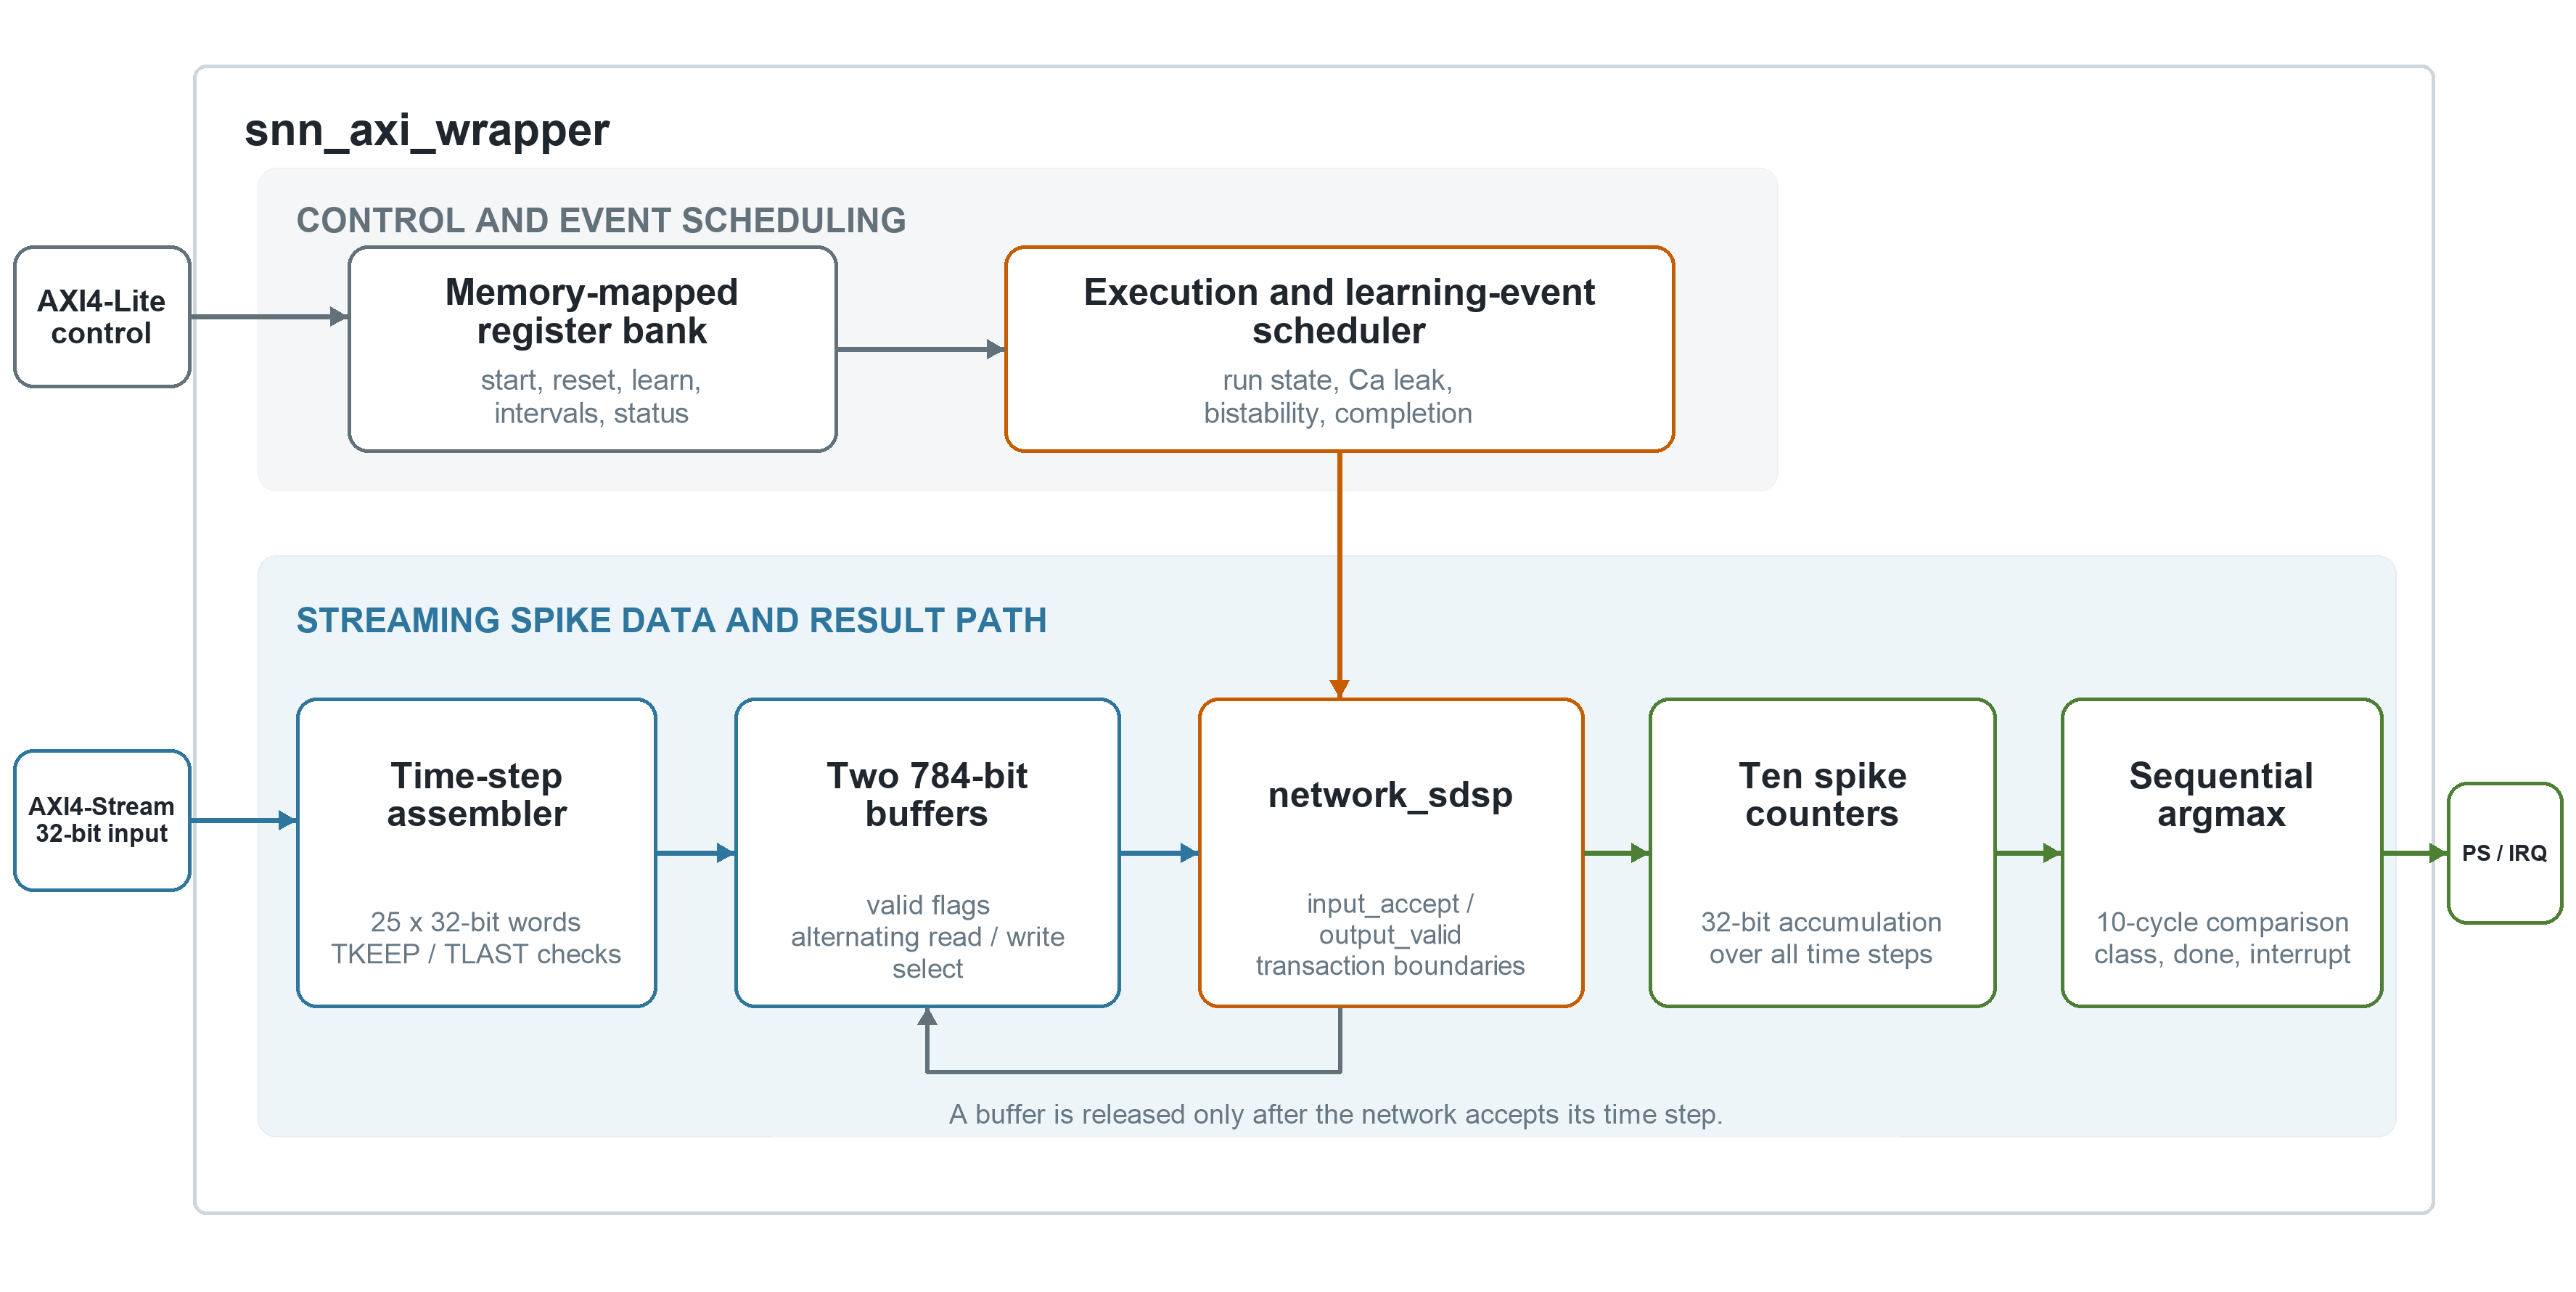
\includegraphics[width=1.10\linewidth]{figures/snn_axi_wrapper_rtl.png}%
	}
	\caption{Implemented Data and Control Flow within \texttt{snn\_axi\_wrapper}}
	\label{fig:snn-axi-wrapper-rtl}
\end{figure}

One network time step contains 784 binary input spikes. The wrapper reconstructs this vector from 25 consecutive 32-bit AXI4-Stream words. Words 0 to 23 contain spike bits 0 to 767, and the lower 16 bits of the final word contain spike bits 768 to 783, while its upper 16 bits serve as padding. The implementation checks \texttt{TKEEP} for every accepted word and expects \texttt{TLAST} only on the final word of the complete input sequence. Unexpected byte enables or an incorrectly positioned \texttt{TLAST} set sticky error flags that can be inspected through the control interface.

Two 784-bit registers form a ping-pong input buffer. The streaming interface assembles a new time step in the buffer selected by \texttt{write\_select}, while the network reads the buffer selected by \texttt{read\_select}. A valid bit is maintained for each buffer. Stream readiness is asserted only when the selected write buffer is empty and the configured number of time steps has not yet been received. Similarly, \texttt{sample\_ready} is presented to the network only when the selected read buffer contains a complete vector. When the network asserts \texttt{input\_accept}, the corresponding valid flag is cleared and the read selection is toggled. Input transfer and network processing can consequently overlap without allowing a partially assembled vector to reach the \gls{snn}.

The AXI4-Lite register bank stores the runtime controls and returns the accelerator status. A start command is retained as \texttt{start\_pending} until both the network and the first input buffer are ready. Dedicated registers hold the learning, teacher, bistability, and interrupt enables, together with the teacher label and current and the calcium-leak and bistability intervals. Countdown registers generate the periodic learning events, avoiding division or modulo operations in the synthesized datapath. A calcium-leak event is issued as a single-cycle pulse, whereas a bistability event remains active for the complete synapse scan so that all excitatory addresses can be examined.

For every valid network output, ten 32-bit counters accumulate the spikes produced by the output neurons. After the final time step has completed, the wrapper determines the output class through a sequential argmax scan. One counter is compared per clock cycle, replacing a long combinational chain of nine comparisons. When the tenth counter has been examined, the wrapper stores the selected class, clears the active state, sets a sticky completion flag, and asserts the interrupt if it has been enabled.

\subsection{Network, Layer, and Neuron RTL}

The \texttt{network\_sdsp} entity preserves the multi-cycle execution model of the generated Spiker+ design. In the implemented configuration, one run contains 100 time steps. The multi-cycle controller requests the next sample only when the modified layer reports that it is ready, and the additional \texttt{sample\_ready} input prevents it from advancing before the AXI wrapper has assembled a complete spike vector. The signals \texttt{input\_accept} and \texttt{out\_spikes\_valid} expose the exact clock cycles at which the input buffer can be released and the corresponding output can be counted.

The layer contains 784 excitatory inputs and ten output neurons. The ten output spikes are also returned as inhibitory inputs, retaining the recurrent competition of the generated network. The multi-input controller scans the excitatory addresses first and subsequently processes the ten inhibitory inputs. For a selected presynaptic address, one 30-bit memory word supplies one three-bit weight to each of the ten neurons. The presynaptic inputs are therefore processed sequentially, while all postsynaptic neurons operate in parallel.

The neuron controller retains the original initialization, excitatory integration, inhibitory integration, leakage, firing, and subtractive-reset operations. Its datapath stores the membrane potential as a 16-bit signed value and exposes this register to the learning comparator. Excitatory weights are represented as unsigned values and are zero-extended before they enter the membrane-potential adder. Inhibitory weights retain their signed representation and are sign-extended. This distinction is required because an excitatory three-bit code with its most significant bit set must remain a positive magnitude rather than being interpreted as a negative two's-complement number.

The neuron-ready signals are combined with the output-barrier status to form the layer-ready condition. The barrier captures the ten output spikes at the end of a time step and retains them for the recurrent inhibitory path. Additional registers record when a step has been accepted and produce a one-cycle \texttt{step\_valid} pulse only after all neuron operations and the barrier transaction have completed. These signals provide the precise transaction boundaries used by the AXI wrapper.

\subsection{Learning Lanes and Synaptic Memory}

The learning hardware is instantiated with a VHDL \texttt{for-generate} statement, producing one learning lane for each output neuron. A lane contains the neuron state, a 3-bit saturating calcium counter, the \gls{sdsp} condition comparator, and the registered weight update datapath. The calcium counter is cleared at the beginning of a new sample, increments on a postsynaptic spike, and decrements on a calcium-leak event. If a spike and a leak event occur in the same clock cycle, the stored value is retained. The comparator treats the calcium value as unsigned and the membrane potential as a signed two's-complement quantity when generating the \texttt{up} and \texttt{down} conditions.

The ten \texttt{sdsp\_top} instances receive the current 30-bit excitatory word as ten independent three-bit fields. Each instance evaluates its local conditions and registers a candidate next weight. The update enable is generated from the global learning enable, the delayed excitatory phase, the validity of the current address, and the presence of either a presynaptic spike or a bistability event. When learning is disabled, the update registers do not alter the stored synaptic state.

Excitatory weights are stored in \texttt{exc\_weight\_ram\_sdsp}, a 784-by-30-bit simple-dual-port memory. Each word contains the ten three-bit weights associated with one presynaptic input. The memory has a synchronous read port and a separate write port on the same clock and is described with read-first behaviour. The \texttt{ram\_style} attribute requests \gls{bram} implementation, and the initialization constants reproduce the weights generated by Spiker+. The inhibitory path is not trained and therefore remains a 10-by-30-bit synchronous read-only memory.

The synchronous read latency is matched to the generated Spiker+ prefetch schedule by three explicit control registers. \texttt{exc\_phase\_d} identifies the excitatory operation whose weight word is currently being consumed, \texttt{write\_addr\_reg} retains its presynaptic address, and \texttt{write\_pending} delays the memory write enable until the corresponding ten updated weights have been registered. The memory can consequently write the completed word for address \(A\) while its read port prefetches address \(A+1\). Retaining the delayed phase also ensures that the update for address 783 is committed after the layer controller leaves the excitatory phase.

This implementation preserves the original sequential-synapse and parallel-neuron organization while adding writable synaptic storage and ten local learning lanes. The complete accelerator remains a synchronous single-clock \gls{rtl} design, and the additional input-accept and output-valid signals provide a deterministic boundary between the AXI wrapper and the modified Spiker+ network.

\section{Vivado Block Design and System Integration}
\label{subsec:block-design-integration}

After the accelerator-specific \gls{rtl} had been completed, the full \texttt{snn\_axi\_wrapper} hierarchy was packaged as a reusable Vivado \gls{ip} core. The packaged core contains the AXI wrapper, the Spiker+-generated network, the modified neuron and memory modules, and all \gls{sdsp} learning logic. Its system-level boundary is therefore limited to one AXI4-Stream slave interface for spike input, one AXI4-Lite slave interface for control and status, a clock, an active-low reset, and one interrupt output. This packaging choice keeps the internal neural-network hierarchy independent of board-level routing while allowing the accelerator to be connected through standard interfaces in Vivado IP Integrator.

Figure \ref{fig:final-block-design} shows the final block design used to generate the PYNQ-Z1 bitstream. The custom accelerator appears as \texttt{snn\_sdsp\_0}. The remaining blocks implement processor access, movement of spike data from DDR memory, stream buffering, synchronized reset generation, and interrupt delivery. Unlike an earlier integration structure in which the accelerator was instantiated beside a generated infrastructure wrapper, the finalized design places the complete accelerator IP directly inside the block design. Vivado subsequently generates \texttt{pynq\_z1\_snn\_sdsp\_wrapper} as the hardware top level, which exposes only the DDR and fixed \gls{ps} connections required by the Zynq device.

\begin{figure}[t]
	\centering
	\makebox[\linewidth][c]{%
		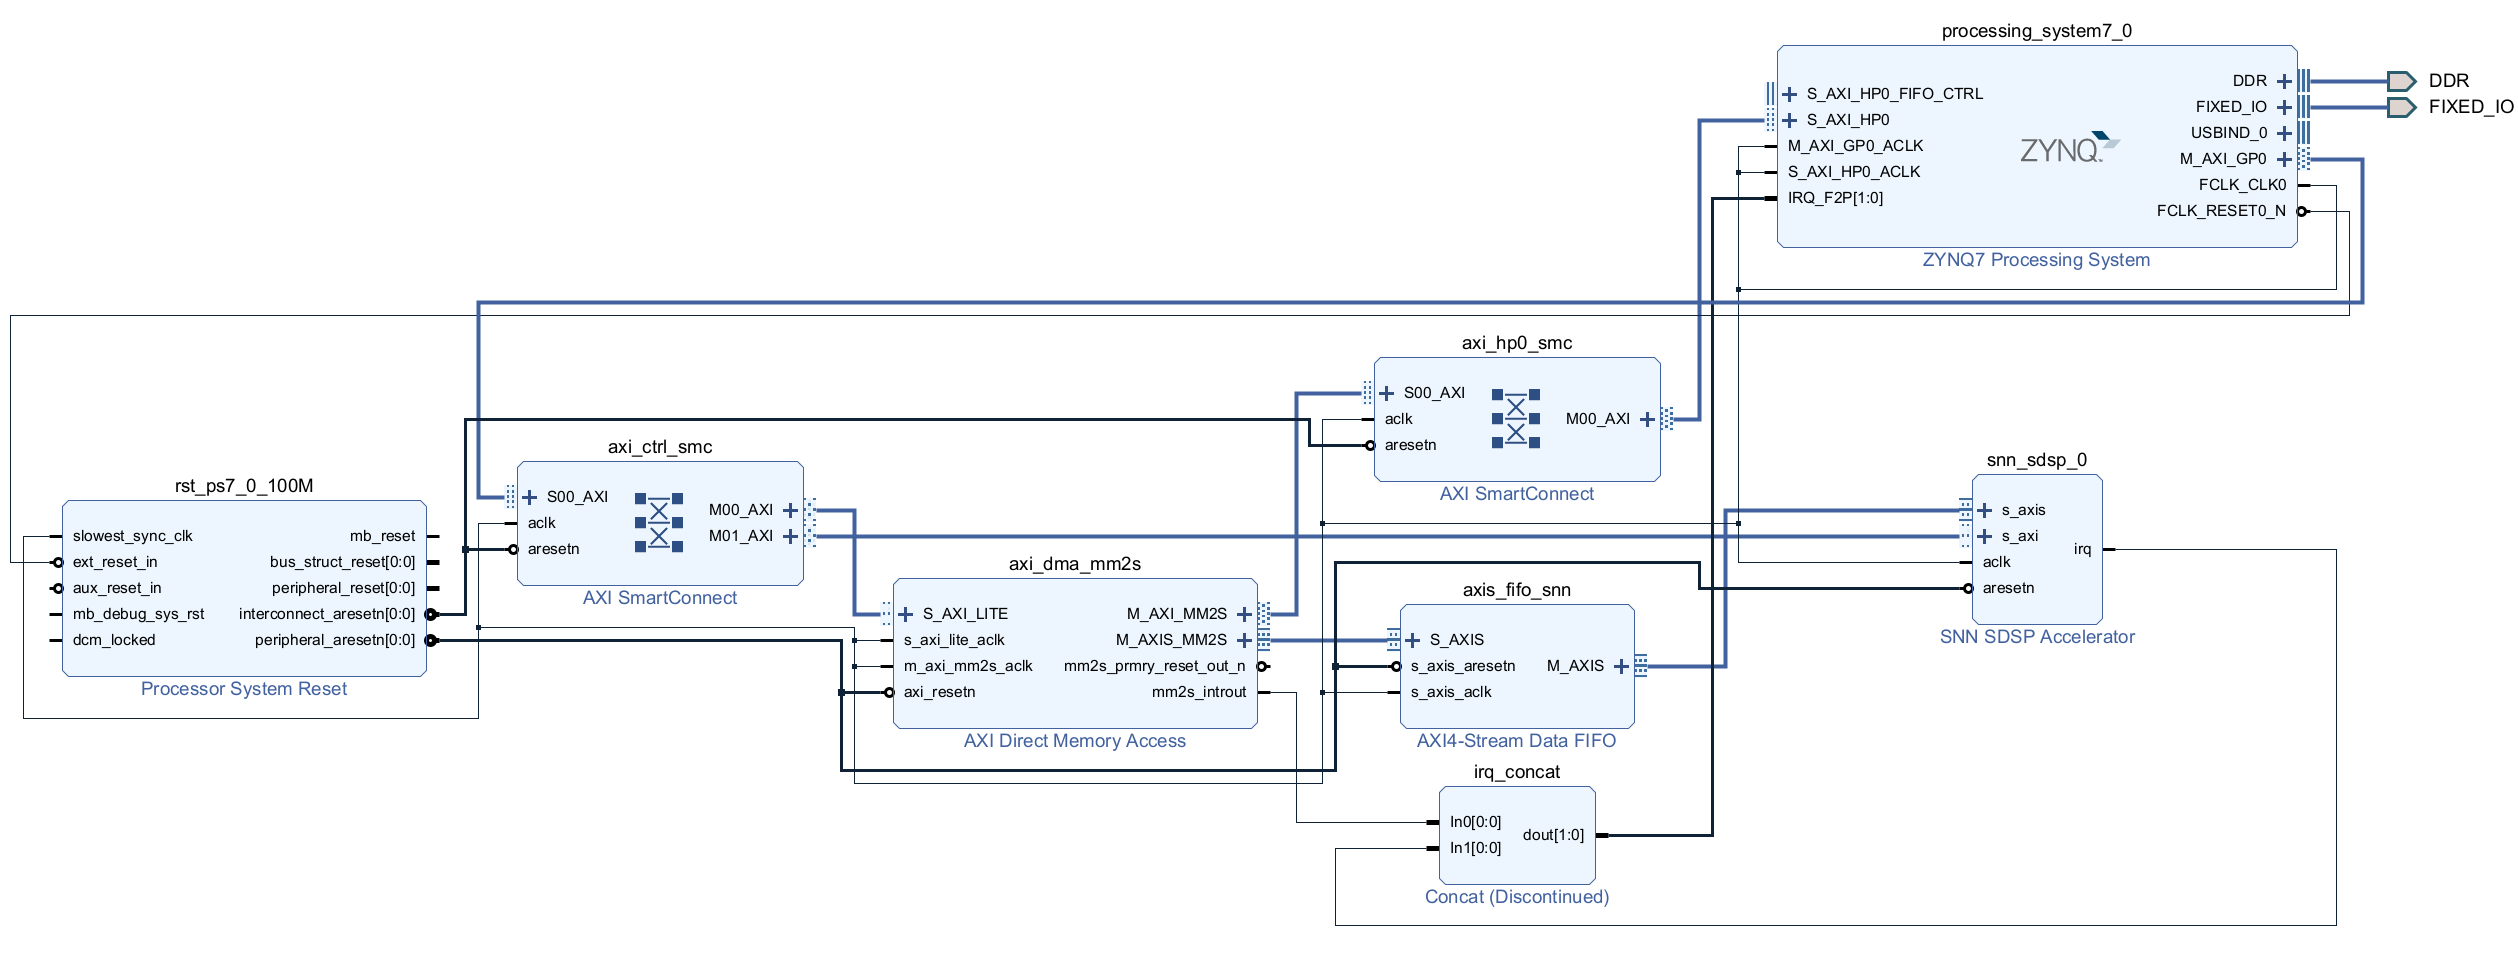
\includegraphics[width=1.06\linewidth]{figures/block_design.png}%
	}
	\caption{Final Vivado Block Design of the PYNQ-Z1 \gls{snn}-\gls{sdsp} System}
	\label{fig:final-block-design}
\end{figure}

\subsection{Control and Data-Movement Paths}

The design separates low-bandwidth control transactions from the bulk input-data transfer. The \gls{ps} accesses the programmable logic through its \texttt{M\_AXI\_GP0} master port. The control SmartConnect, \texttt{axi\_ctrl\_smc}, decodes this address space and provides two subordinate paths: one to the AXI-Lite control port of \texttt{axi\_dma\_mm2s} and one to the AXI-Lite slave port of \texttt{snn\_sdsp\_0}. Software can consequently configure the DMA and the accelerator independently through memory-mapped accesses.

Input spike trains are prepared in external DDR memory. The AXI DMA is configured in simple, memory-to-stream mode; its stream-to-memory channel and scatter-gather engine are not included because the accelerator returns its classification result and status through AXI-Lite rather than through an output stream. On the memory side, the DMA uses a 64-bit AXI master interface. Its read requests reach DDR through \texttt{axi\_hp0\_smc} and the high-performance \texttt{S\_AXI\_HP0} port of the processing system. On the stream side, the DMA emits 32-bit words containing \texttt{TKEEP} and \texttt{TLAST}, matching the input interface of the packaged accelerator.

An AXI4-Stream Data FIFO is inserted between the DMA and \texttt{snn\_sdsp\_0}. The FIFO stores up to 512 stream words and propagates both \texttt{TKEEP} and \texttt{TLAST}. Its purpose is to decouple burst-oriented DDR transfers from the accelerator's input backpressure. The DMA can therefore continue filling the FIFO while the two internal spike-vector buffers are temporarily occupied, provided that sufficient FIFO capacity remains. The FIFO does not alter the word order or packet boundary; reconstruction and validation of the 784-bit input vectors remain the responsibility of \texttt{snn\_axi\_wrapper}, as described in Section \ref{subsec:rtl-architecture}.

Table \ref{tab:block-design-address-map} summarizes the address assignments generated for the final block design. The two 64-KiB control regions are visible to the processing system through \texttt{M\_AXI\_GP0}. The DMA can read the lower 512 MiB of the processing-system memory map through the HP0 data path. Keeping control and data movement on separate AXI paths prevents the repeated spike-data reads from sharing the low-bandwidth register path used for configuration and result access.

\begin{table}[htbp]
	\centering
	\caption{Address Map of the Final Vivado Block Design}
	\label{tab:block-design-address-map}
	\small
	\begin{tabularx}{\linewidth}{@{}l l l X@{}}
		\toprule
		\textbf{Access path} & \textbf{Base address} & \textbf{Span} & \textbf{Purpose} \\
		\midrule
		PS GP0 to DMA & \texttt{0x4040\_0000} & 64 KiB & Configuration and status of the MM2S DMA channel \\
		PS GP0 to accelerator & \texttt{0x43C0\_0000} & 64 KiB & Accelerator control, learning configuration, status, spike counts, and classification result \\
		DMA to PS HP0 & \texttt{0x0000\_0000} & 512 MiB & Reading the input spike buffer from external DDR memory \\
		\bottomrule
	\end{tabularx}
\end{table}

\subsection{Clock and Reset Distribution}

The processing system generates \texttt{FCLK\_CLK0} at 100\,MHz. This clock drives the GP0 and HP0 AXI interfaces, both SmartConnect instances, the memory-mapped and streaming sides of the DMA, the stream FIFO, and the packaged accelerator. Using a common clock for the complete programmable-logic data path avoids additional clock-domain-crossing logic and keeps the AXI handshakes aligned with the internal network schedule.

The active-low \texttt{FCLK\_RESET0\_N} signal enters the Processor System Reset IP shown in Figure \ref{fig:final-block-design}. This block synchronizes reset release to the fabric clock and produces separate active-low reset nets for the interconnect and peripheral groups. The interconnect reset is connected to the two SmartConnect blocks, while the peripheral reset initializes the DMA, stream FIFO, and accelerator IP. This arrangement ensures that no AXI endpoint begins a transaction before its associated interconnect has left reset. The accelerator's software-triggered reset remains internal to \texttt{snn\_axi\_wrapper}; it clears the network and transaction state without resetting the surrounding DMA or AXI fabric.

\subsection{Interrupt Integration and Runtime Sequence}

Two programmable-logic interrupts are returned to the processing system. The DMA's \texttt{mm2s\_introut} signal is connected to input 0 of \texttt{irq\_concat}, and the accelerator interrupt is connected to input 1. The resulting two-bit vector drives \texttt{IRQ\_F2P[1:0]}. Keeping the two sources separate allows processor-side software to distinguish completion or error events generated by the DMA from completion of the neural-network transaction. Within the accelerator, the interrupt is asserted when the classification result has been committed and the interrupt-enable control bit is set. It remains asserted through the sticky completion state until software clears that state.

At runtime, the processor first loads the overlay and places the packed input spike sequence in a contiguous DDR buffer. It then programs the learning enable, teacher enable, target label, teacher current, and learning-event intervals through the accelerator's AXI-Lite register space, configures the MM2S transfer, and issues the accelerator start command. The DMA reads the buffer through HP0 and streams the words through the FIFO into the packaged IP. After all configured time steps have been accepted and processed, the accelerator completes its sequential output scan, stores the winning class and individual spike counts, and raises its interrupt when enabled. The processor can then read the result through AXI-Lite without requiring a return DMA channel. This transaction sequence confines high-volume movement to the DDR-to-stream path and retains deterministic online learning entirely inside the programmable logic.

\section{PYNQ Runtime Control and Data Preparation}
\label{subsec:pynq-runtime-control}

The processor-side runtime provides the operational boundary between an experiment and the hardware system described in Section \ref{subsec:block-design-integration}. Its responsibilities are limited to loading the overlay, preparing the spike representation expected by the AXI wrapper, configuring one accelerator transaction, and retrieving its results. Membrane integration and synaptic-weight updates are not reproduced in software. Consequently, the processor remains outside the time-critical learning loop and the behaviour of \gls{sdsp} is determined by the programmable-logic implementation.

Figure \ref{fig:pynq-runtime-workflow} summarizes the resulting workflow. Control and status use AXI4-Lite, whereas the substantially larger spike sequence is transferred from DDR through the MM2S DMA path. This separation allows the same allocated input buffer and overlay instance to be reused across multiple samples while the software changes only the sample data and the run-specific control values.

\begin{figure}[t]
	\centering
	\makebox[\linewidth][c]{%
		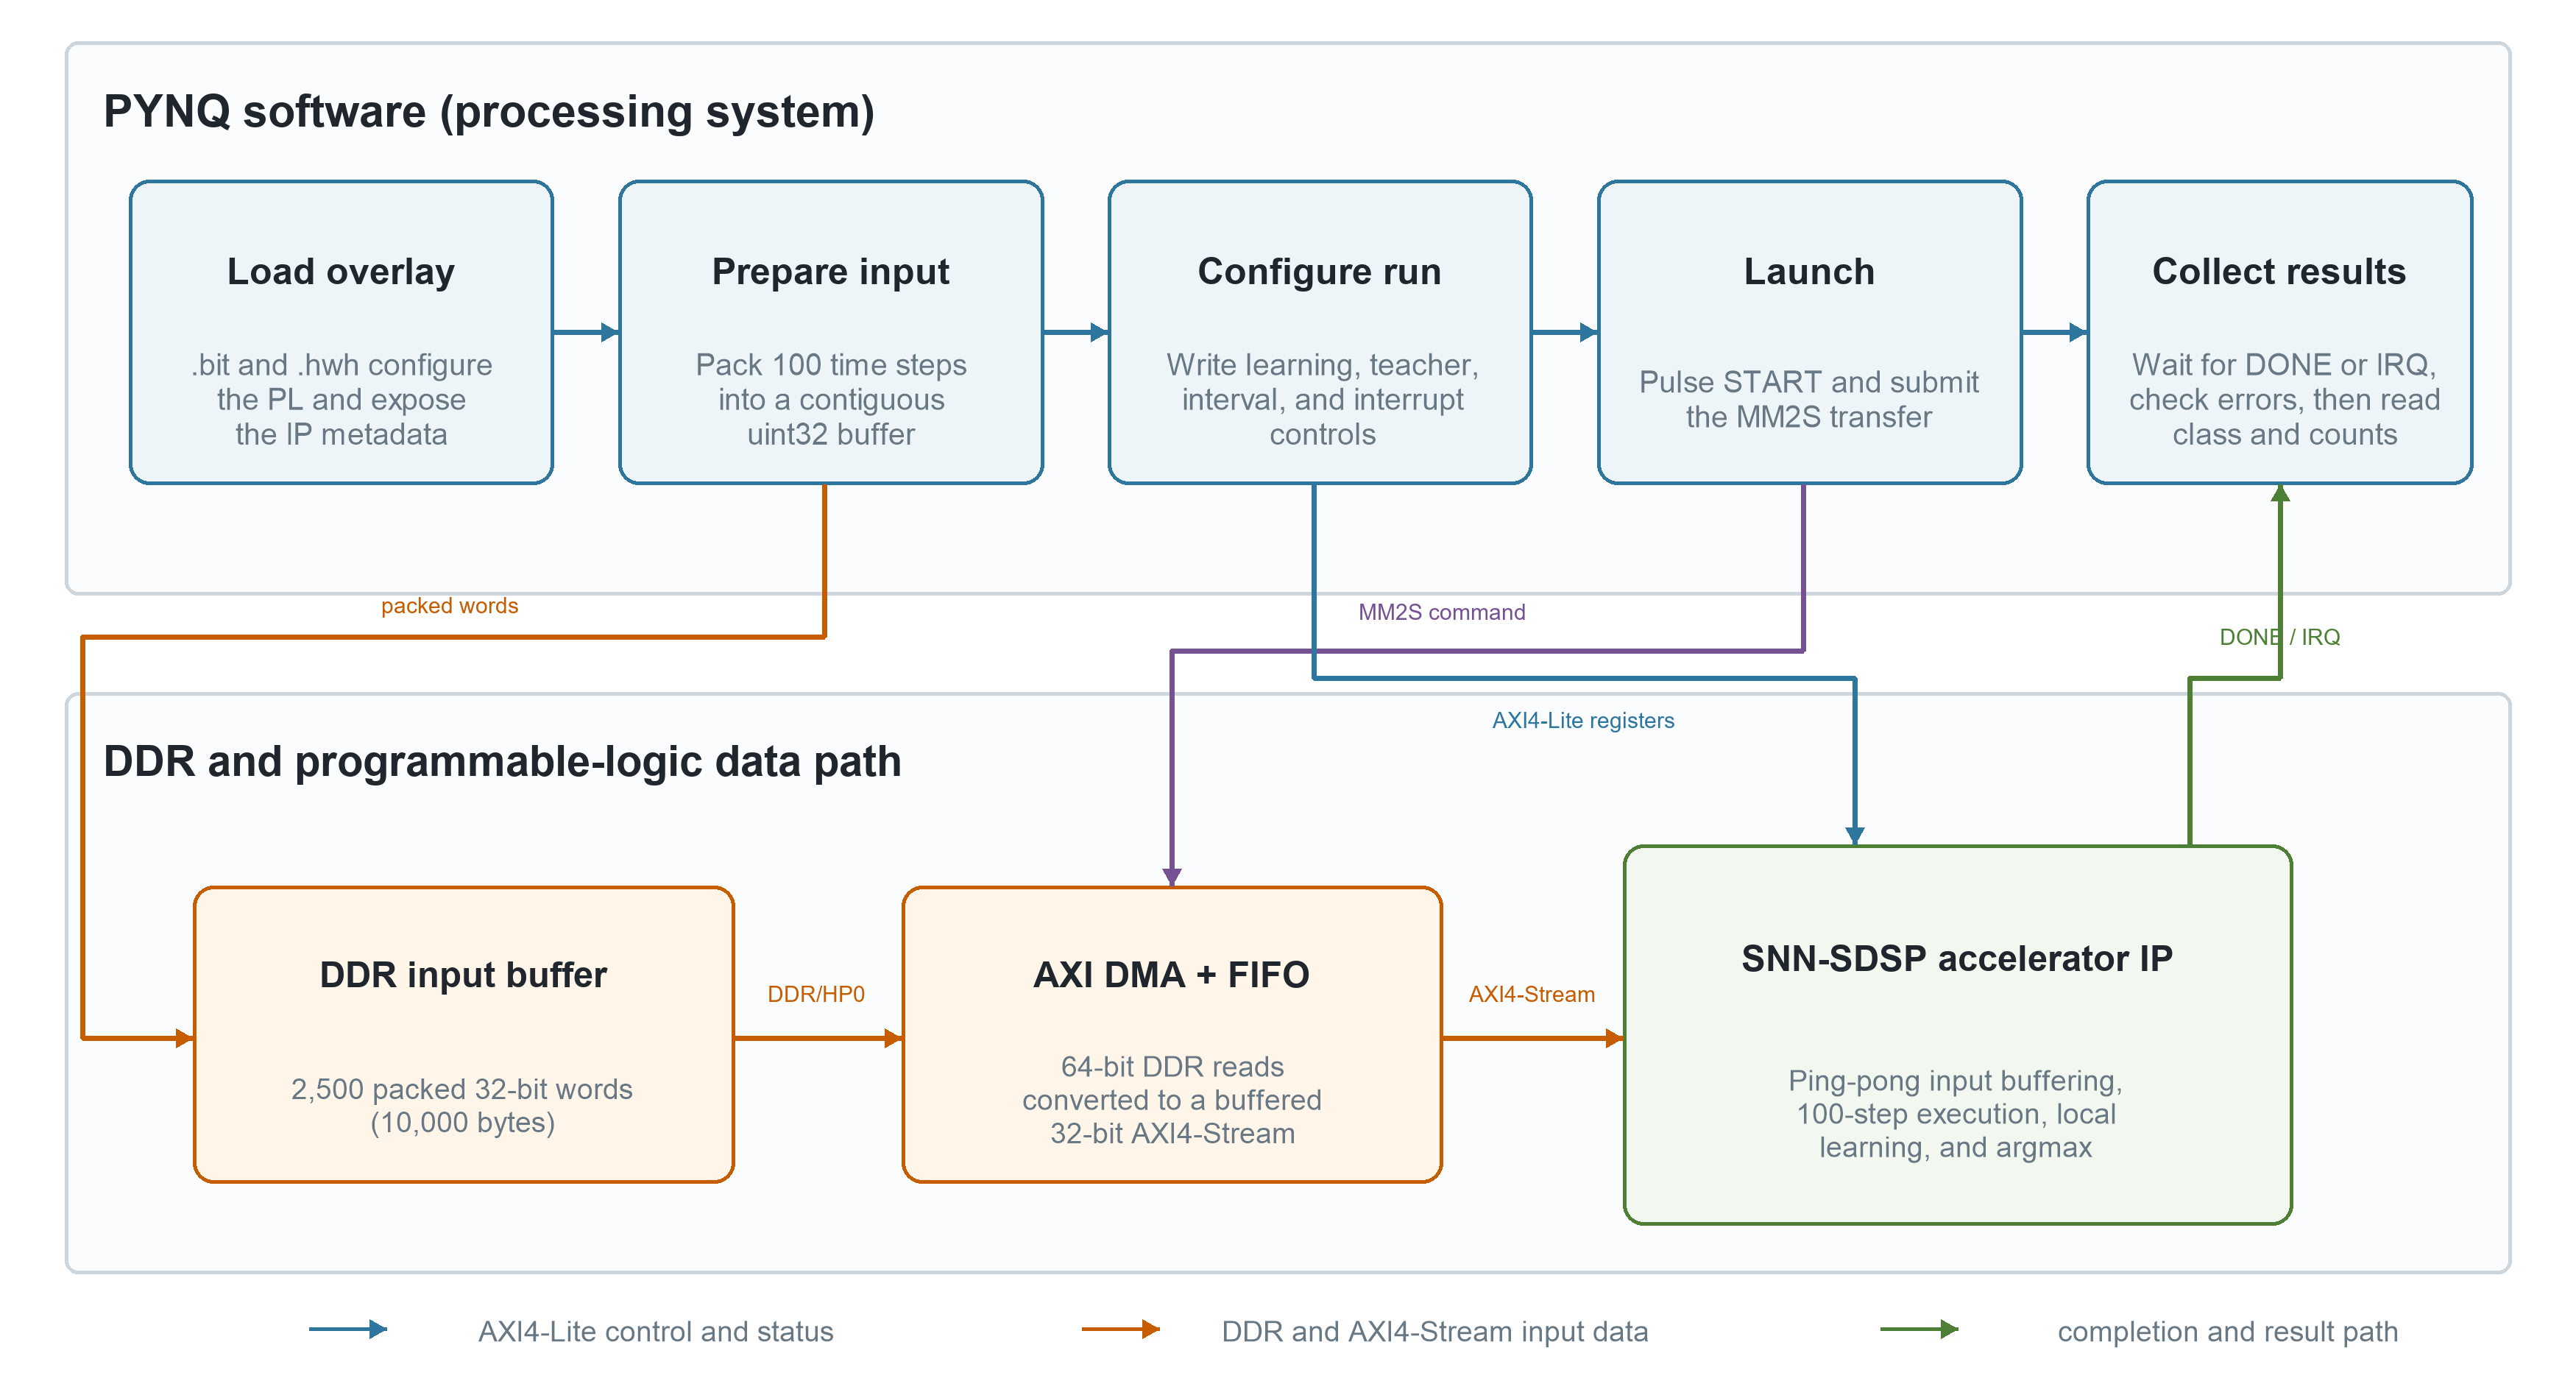
\includegraphics[width=1.06\linewidth]{figures/pynq_runtime_workflow.png}%
	}
	\caption{End-to-End PYNQ Runtime Workflow for One Accelerator Transaction}
	\label{fig:pynq-runtime-workflow}
\end{figure}

\subsection{Overlay Initialization and Register Interface}

The generated bitstream and hardware handoff file are deployed with the same overlay name. Loading the bitstream through the PYNQ \texttt{Overlay} class configures the programmable logic, while the \texttt{.hwh} metadata makes the DMA, accelerator address space, and interrupt connections visible to Python \cite{PYNQOverlayLoading}. The final design exposes the two relevant blocks as \texttt{axi\_dma\_mm2s} and \texttt{snn\_sdsp\_0}. A dedicated software driver is not required for the custom accelerator because its command and result registers can be accessed through the memory-mapped interface provided by the overlay.

Table \ref{tab:snn-axi-register-map} lists the implemented accelerator registers. The control register combines single-cycle commands with persistent mode bits. \texttt{START}, \texttt{SOFT\_RESET}, and \texttt{CLEAR\_DONE} are interpreted as command pulses, whereas the learning, bistability, interrupt, and teacher enables remain stored until software changes them. The target label, teacher current, and enable state are written before \texttt{START}; the teacher-related values are then captured for the complete transaction so that later processor writes cannot change supervision while a sample is being processed.

\begin{table}[htbp]
	\centering
	\caption{Software-Visible Register Map of \texttt{snn\_sdsp\_0}}
	\label{tab:snn-axi-register-map}
	\small
	\begin{tabularx}{\linewidth}{@{}l l X@{}}
		\toprule
		\textbf{Offset} & \textbf{Access} & \textbf{Function} \\
		\midrule
		\texttt{0x00} & R/W & Control: start, soft reset, learning enable, bistability enable, interrupt enable, completion clear, and teacher enable \\
		\texttt{0x04} & R & Status: idle, busy, completion, stream-format errors, active state, and input-buffer validity \\
		\texttt{0x08} & R & Number of time steps configured in the hardware instance \\
		\texttt{0x0C} & R/W & Four-bit target class used for teacher supervision \\
		\texttt{0x10} & R/W & Calcium-leak event interval \\
		\texttt{0x14} & R/W & Bistability event interval \\
		\texttt{0x18} & R/W & Teacher-current value applied to the selected output neuron \\
		\texttt{0x20} & R & Classification result produced by the final argmax scan \\
		\texttt{0x24--0x48} & R & Ten 32-bit output-neuron spike counters \\
		\texttt{0x50} & R & Number of input time steps accepted by the network \\
		\texttt{0x54} & R & Stream and execution progress, including word and completed-step counters \\
		\bottomrule
	\end{tabularx}
\end{table}

The status and progress registers also support debugging without introducing signals at the board boundary. In normal operation, software needs only the busy, completion, and error flags. The accepted-step and progress values are useful when distinguishing malformed input data from a stalled network transaction. A soft reset can clear the network and wrapper state without reconfiguring the complete overlay. It does not reload the initialized excitatory memory, so learned weights remain available for subsequent samples until the programmable logic is reconfigured.

\subsection{Spike Packing and DMA Transfer}

The input representation is prepared as an array of unsigned 32-bit words. Each 784-neuron time step occupies 25 words: the first 24 words carry 768 spike bits, and the lower 16 bits of the final word carry the remaining spikes. The unused upper half of the final word is set to zero. With the implemented value of 100 time steps, one accelerator transaction therefore contains 2,500 words, corresponding to 10,000 bytes. Software can read the configured time-step count from offset \texttt{0x08} instead of duplicating this value as a separate runtime constant.

The packed array is placed in a physically contiguous PYNQ buffer created with \texttt{pynq.allocate}, which provides the memory layout and device-visible address required by the DMA \cite{PYNQBuffer}. After the array has been populated, its contents are synchronized to the device when required by the selected memory configuration. The PYNQ DMA interface then submits the complete buffer to the MM2S channel \cite{PYNQDMA}. The transfer length defines the AXI4-Stream packet, causing \texttt{TLAST} to accompany only its final word. All transferred words contain four valid bytes, matching the \texttt{TKEEP=1111} check performed by \texttt{snn\_axi\_wrapper}.

No processor-side throttling is required between individual time steps. Backpressure from the accelerator propagates through the AXI4-Stream FIFO to the DMA, while the two internal input buffers allow transmission and neural processing to overlap. The software therefore submits one contiguous transaction rather than repeatedly controlling the DMA for each 784-bit vector. This both reduces processor involvement and preserves the packet boundary checked by the hardware.

\subsection{Transaction Completion and Result Retrieval}

Before starting a sample, software clears a previous completion flag and programs the desired operating mode. For inference, learning and teacher supervision are disabled. For online learning, software additionally writes the target label, teacher current, calcium-leak interval, and optional bistability configuration. These values must be valid before the \texttt{START} pulse because the supervision parameters are captured when the new transaction is accepted.

The start request may be issued before the first stream word arrives. In this case, the wrapper retains it as \texttt{start\_pending} and activates the network only after one complete time-step vector is available. Software can therefore launch the accelerator and the MM2S transfer without cycle-level coordination. During execution, the DMA and accelerator interrupts remain independent: the DMA interrupt indicates completion of the memory-to-stream transfer, whereas the accelerator interrupt indicates that all network outputs have been processed and the classification result is valid.

Completion can be detected either by waiting for the accelerator interrupt or by polling the completion bit at offset \texttt{0x04}. The stream and \texttt{TLAST} error flags are checked before the result is accepted. Software then reads the predicted class from offset \texttt{0x20} and, when detailed evaluation is required, the ten spike counters from offsets \texttt{0x24} to \texttt{0x48}. Finally, \texttt{CLEAR\_DONE} acknowledges the completed transaction. The same overlay and allocated buffer can then be reused for the next sample; only reloading the bitstream restores the original initialized synaptic weights.

\section{Verification Infrastructure and Test Strategy}
\label{subsec:verification-infrastructure}

Verification was organized as a sequence of increasingly integrated checks rather than as a single end-to-end simulation. This structure was necessary because an incorrect final classification can originate from several different sources, including the learning rule, the generated network schedule, AXI stream framing, or processor-side data preparation. Exercising these boundaries independently makes a failure observable close to its source and reduces the number of internal signals that must be inspected at the system level.

Figure \ref{fig:verification-strategy} shows the four verification levels used for the implementation. Module-level tests establish the behaviour of the learning primitives and writable memory. Layer and network tests then check the timing contracts inherited from Spiker+. AXI-wrapper tests verify the complete hardware transaction boundary, while the final level compares board-produced observations with a software reference using preserved input data. Quantitative results obtained with this infrastructure are reported in Chapter \ref{sec:results_and_evaluation}; this section describes only how the checks were constructed.

\begin{figure}[t]
	\centering
	\makebox[\linewidth][c]{%
		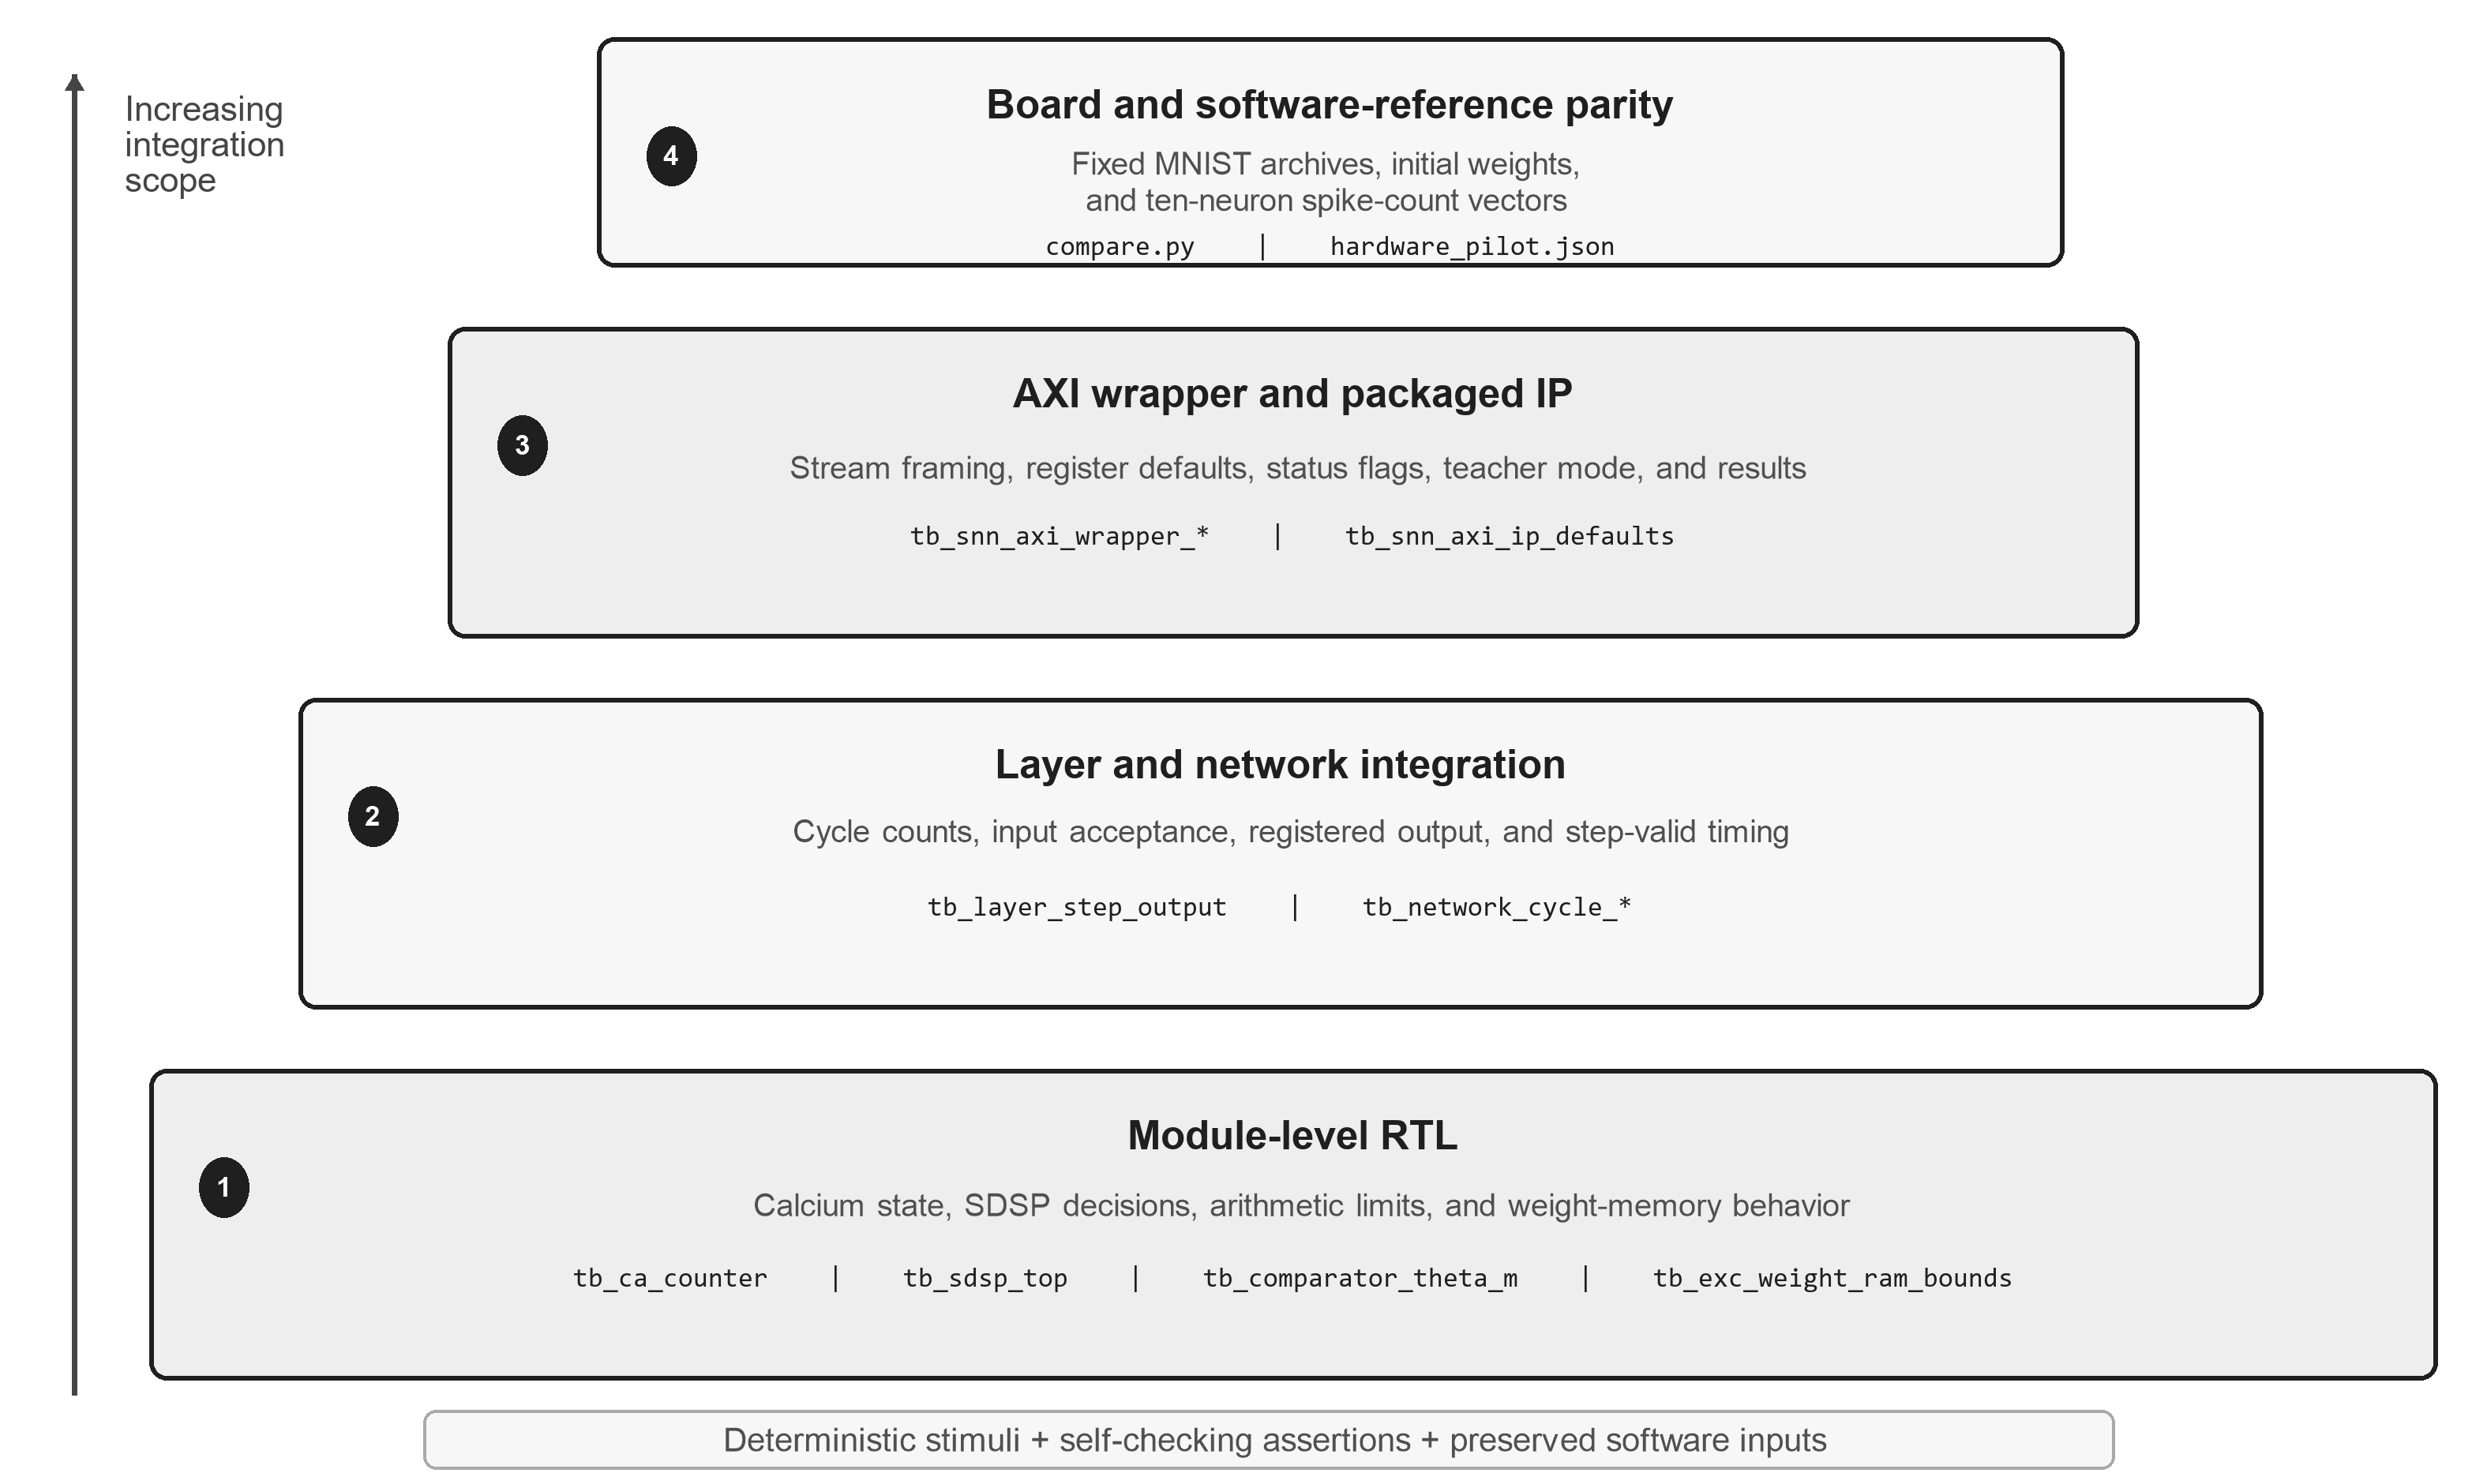
\includegraphics[width=1.04\linewidth]{figures/verification_strategy.png}%
	}
	\caption{Layered Verification Strategy for the Implemented System}
	\label{fig:verification-strategy}
\end{figure}

\subsection{Module-Level RTL Verification}

The lowest verification level uses self-checking VHDL testbenches for the individual \gls{sdsp} building blocks. The calcium counter tests exercise reset, increments caused by postsynaptic spikes, leak events, simultaneous spike-and-leak handling, and saturation at the representable limits. The condition comparator is tested around the signed membrane-potential threshold and the calcium boundaries, ensuring that the generated \texttt{up} and \texttt{down} conditions change at the intended encoded values. Separate tests cover the delta-weight generator, full-adder-based update path, overflow handling, and the integrated \texttt{sdsp\_top} unit.

The writable excitatory memory receives an additional boundary test because its address range is narrower than the ten-bit address signal. The testbench reads the first and final valid entries, checks that the unused prefetched address returns a defined zero value, and verifies read-first behaviour during a weight write. These checks directly target the last-address condition created by the Spiker+ prefetch schedule. A separate synthesis script checks that the 784-by-30-bit description is inferred as block memory; functional simulation alone cannot establish the selected FPGA storage primitive.

All unit tests use assertions rather than relying only on waveform inspection. A mismatch therefore terminates the simulation at the first violated property and identifies the expected interface contract. Waveforms remain useful for diagnosing a failure, but they are not the sole acceptance criterion.

\subsection{Network and AXI Integration Tests}

The second level verifies the interfaces between the generated controller, the modified layer, and the network wrapper. Cycle-count testbenches count the \texttt{sample}, \texttt{input\_accept}, and \texttt{out\_spikes\_valid} events and compare them with the configured number of time steps. The layer-output testbench separately checks that the output exported with \texttt{step\_valid} is the value already captured by the output barrier. This isolates the network schedule from AXI behaviour and verifies the transaction boundaries used by the ping-pong buffers.

At the wrapper level, AXI4-Stream stimuli reproduce the same 25-word representation used on the board. Short two-step tests provide rapid feedback for handshakes, word assembly, completion state, and result access. The full-size test transfers 2,500 words and checks the accepted- and completed-step counts for a 100-step transaction. Its selectable stimulus modes cover the normal sparse stream, dense input activity, zero-input control behaviour, and teacher-enabled zero-input operation. The dense case makes the output path observable, while the paired teacher-enabled and teacher-disabled cases isolate the contribution of the supervision current.

AXI-Lite accesses are generated by reusable write and read procedures inside the testbenches. They configure the same registers used by PYNQ software and subsequently inspect status, progress, classification, and spike-count values. An additional packaged-IP test verifies that customization defaults appear after hardware reset, that processor writes override them, and that reset restores the configured defaults. Table \ref{tab:verification-artifacts} summarizes the representative verification artifacts and their primary checks. Together, these tests cover both the internal computation schedule and the software-visible contract of \texttt{snn\_sdsp\_0}.

\begin{table}[htbp]
	\centering
	\caption{Representative Verification Artifacts and Their Primary Checks}
	\label{tab:verification-artifacts}
	\small
	\begin{tabularx}{\linewidth}{@{}p{0.20\linewidth}p{0.34\linewidth}X@{}}
		\toprule
		\textbf{Scope} & \textbf{Representative artifact} & \textbf{Primary check} \\
		\midrule
		SDSP modules & \texttt{tb\_ca\_counter}, \texttt{tb\_sdsp\_top} & State transitions, update selection, saturation, and event handling \\
		Comparator and RAM & \texttt{tb\_comparator\_theta\_m}, \texttt{tb\_exc\_weight\_ram\_bounds} & Signed threshold boundary, valid address range, read-first semantics, and write-back \\
		Layer and network & \texttt{tb\_layer\_step\_output}, \texttt{tb\_network\_cycle\_count} & Registered output alignment and agreement between requested, accepted, and completed steps \\
		AXI wrapper & \texttt{tb\_snn\_axi\_wrapper\_two\_steps}, \texttt{tb\_snn\_axi\_wrapper\_100\_steps} & Stream handshakes, packet assembly, modes, status, results, and completion \\
		Packaged IP & \texttt{tb\_snn\_axi\_ip\_defaults} & IP customization defaults, AXI register overrides, and reset restoration \\
		Cross-domain comparison & \texttt{compare.py} & Input identity, initial-weight decoding, and per-neuron spike-count comparison \\
		\bottomrule
	\end{tabularx}
\end{table}

\subsection{Hardware--Software Parity and Reproducibility}

The highest verification level compares observations from the deployed design with the Spiker+ software model. The comparison uses stored spike archives rather than regenerating stochastic spike trains for each run. Each archive records the packed words, labels, time-step count, gain, and bit order, while a SHA-256 digest identifies the exact training input used by the board experiment. Preserving the input realization is essential because two independently generated stochastic encodings of the same image do not provide a sample-by-sample comparison.

The comparison script decodes the VHDL initialization package into the same ten-by-784 weight matrix used by the software model. It first checks the weight-code distribution and verifies whether the software and hardware initial states are identical. It then applies the preserved input words to the software model and compares the ten output-neuron spike counts with the board observations. Comparing the complete count vector is more informative than comparing only the winning class, since different internal behaviour can still produce the same argmax result.

This parity step is intentionally treated as a diagnostic comparison rather than as proof of cycle-accurate equivalence. The software model uses floating-point neuron dynamics, whereas the implemented datapath uses fixed-point arithmetic and an explicit multi-cycle schedule. Any remaining difference must therefore be interpreted together with the lower verification levels. The script prevents a training comparison from being presented as exact parity unless the initial-state and baseline conditions have first been established; an explicitly forced run is labelled only as a trend comparison.

Board observations are stored separately from the comparison script, and the script does not reprogram the device or modify the preserved data. This separation makes the experiment repeatable and prevents a software rerun from silently changing the hardware stimulus. The same fixed evaluation archive can consequently be used before and after online learning, allowing changes in the output distribution to be attributed to the learned synaptic state rather than to a different stochastic input realization.

\section{Chapter Summary}
\label{subsec:implementation-summary}

This chapter presented the implementation of the proposed online-learning \gls{snn} on the PYNQ-Z1 platform. The Spiker+-generated network, the modified neuron and synaptic-memory modules, and the \gls{sdsp} learning logic were integrated beneath \texttt{snn\_axi\_wrapper} and packaged as a reusable Vivado \gls{ip} core. The final block design connects this accelerator to the Zynq processing system through an AXI4-Lite control path, an AXI DMA and stream FIFO for spike-data transfer, a shared clock and reset structure, and separate DMA and accelerator interrupts.

On the processor side, the PYNQ overlay and runtime interface provide input preparation, register configuration, transaction control, and result retrieval, while spike processing and synaptic updates remain inside the programmable logic. A layered verification environment was established from self-checking module simulations through network and AXI integration tests to board-level comparison with preserved software inputs. Together, these implementation and verification components provide the deployable system used for the functional, resource, timing, and learning evaluations presented in Chapter \ref{sec:results_and_evaluation}.

% !TEX root = thesis.tex
\chapter{Results and Evaluation}
\label{sec:results_and_evaluation}

This chapter evaluates the implemented \gls{snn} accelerator at both the hardware and application levels. It first verifies the correct operation of the processor--programmable-logic communication path, the accelerator interfaces, and the online weight-update mechanism. The implementation is then assessed in terms of \gls{fpga} resource utilization, timing performance, and end-to-end processing speed. Finally, the learning capability is evaluated using three complete training epochs on the MNIST dataset, followed by an analysis of classification accuracy, output activity, and class-dependent behaviour. The obtained results are compared with representative \gls{sdsp}-based hardware, with particular attention to TEDOP and to differences in neuron models, learning rules, data preparation, numerical precision, and measurement boundaries. The chapter concludes by discussing the significance and limitations of the results, particularly the use of a single-layer network and the limited number of training epochs.

\section{Experimental Setup and Evaluation Methodology}
\label{subsec:experimental-setup}

The evaluation was designed to separate three questions. First, the board-level tests determine whether the deployed accelerator accepts correctly formatted input transactions and exposes valid status and result information. Second, controlled learning tests determine whether teacher-guided \gls{sdsp} updates produce a persistent change in network behaviour. Third, complete MNIST training epochs assess whether these local updates improve classification performance over a larger workload. The following configuration and protocol were kept fixed so that changes observed between evaluations can be attributed to the learned synaptic state rather than to a change in the hardware or input representation.

\subsection{Hardware and Network Configuration}

All measurements use the final PYNQ-Z1 overlay described in Chapter \ref{sec:implementation}. The \gls{ps} loads the prepared spike data from storage, places one encoded image in a contiguous \gls{ddr} \gls{sdram} buffer, configures the accelerator through AXI4-Lite, and starts the memory-to-stream \gls{dma} transfer. The \gls{pl} receives the complete 100-step input sequence, executes the generated network schedule, performs local weight updates when learning is enabled, and records the output-neuron spike counts. Consequently, the reported board-level measurements include the complete implemented path rather than an isolated simulation of the learning rule.

The evaluated network contains 784 external inputs and ten \gls{lif} output neurons. No hidden layer is used. This configuration keeps the hardware experiment focused on the integration of online learning and provides the same input--output dimensions as the single-layer TEDOP network used later for comparison. The output spikes are also returned through the fixed inhibitory path to preserve the competition mechanism of the generated Spiker+ design. The topology choice and its implications for classification accuracy are discussed later in this chapter.

Table \ref{tab:evaluation-configuration} summarizes the configuration used throughout the board experiments. The teacher current is represented in the accelerator's fixed-point format. Its register value of 128 corresponds to 0.25 in Q9 representation. Calcium leakage is generated once every ten network time steps, while bistability events are disabled. These values were held constant across all three training epochs; the experiment therefore evaluates one defined hardware configuration rather than a parameter sweep.

\begin{table}[htbp]
	\centering
	\caption{Configuration Used for the Board-Level Evaluation}
	\label{tab:evaluation-configuration}
	\small
	\begin{tabularx}{\linewidth}{@{}p{0.32\linewidth}X@{}}
		\toprule
		\textbf{Item} & \textbf{Evaluation configuration} \\
		\midrule
		Target platform & PYNQ-Z1 with an XC7Z020 device \\
		Programmable-logic clock & 100\,MHz \\
		Network topology & 784 external inputs and ten output neurons, without a hidden layer \\
		Neuron model & Modified subtractive-reset \gls{lif} neuron with recurrent output inhibition \\
		Input duration & 100 network time steps per image \\
		Spike encoding & Rate coding using the Spiker+ MNIST data loader with a gain of 0.1 \\
		Input transaction & 25 32-bit words per time step; 2,500 words or 10,000 bytes per image \\
		Excitatory weights & 3-bit unsigned weights stored as a 784-by-30-bit memory \\
		Learning mode & Teacher-guided \gls{sdsp} enabled during training and disabled during evaluation \\
		Teacher current & Register value 128, corresponding to 0.25 in Q9 representation \\
		Calcium leakage & One leak event every ten network time steps \\
		Bistability & Disabled \\
		Output decision & Index of the output neuron with the largest spike count \\
		\bottomrule
	\end{tabularx}
\end{table}

\subsection{Dataset Preparation and Experimental Protocol}

The application-level evaluation uses the MNIST handwritten-digit dataset, which provides separate training and test partitions \cite{LeCun1998GradientBasedLearning}. The complete set of 60,000 training images is presented once in each epoch. To retain the stochastic behaviour of rate coding, the image order and the generated spike realization are produced independently for every epoch. Seeds 2028, 2029, and 2030 are used for epochs one to three, respectively. Each resulting archive contains 60 ordered shards of 1,000 images. The archive manifest records the encoding parameters, label distribution, and input-spike count, while a SHA-256 digest is checked after transfer to the board. This prevents an incomplete or different archive from being used unnoticed.

A separate class-balanced subset of 1,000 images is selected from the MNIST test partition using seed 2027. It contains 100 images from each digit class and excludes the first ten test images that had previously been used for small functional checks. Unlike the training inputs, this set is encoded only once and stored as a fixed spike archive. Reusing the identical packed words before training and after every epoch removes stochastic re-encoding as a cause of differences between evaluation points.

Figure \ref{fig:evaluation-protocol} shows the resulting experimental sequence. The bitstream is first loaded once to restore the initial weights, after which a baseline evaluation is performed. Training and evaluation then alternate for three epochs. Learning and teacher input are enabled only for the 60,000 training transactions of an epoch. Both are disabled when the fixed 1,000-image set is evaluated. The FPGA is not reprogrammed between epochs, because doing so would restore the initialized weight memory and discard the learning achieved by the preceding epoch. A soft reset before an image clears the transaction and neural state required for a new sample without replacing the learned synaptic weights.

\begin{figure}[t]
	\centering
	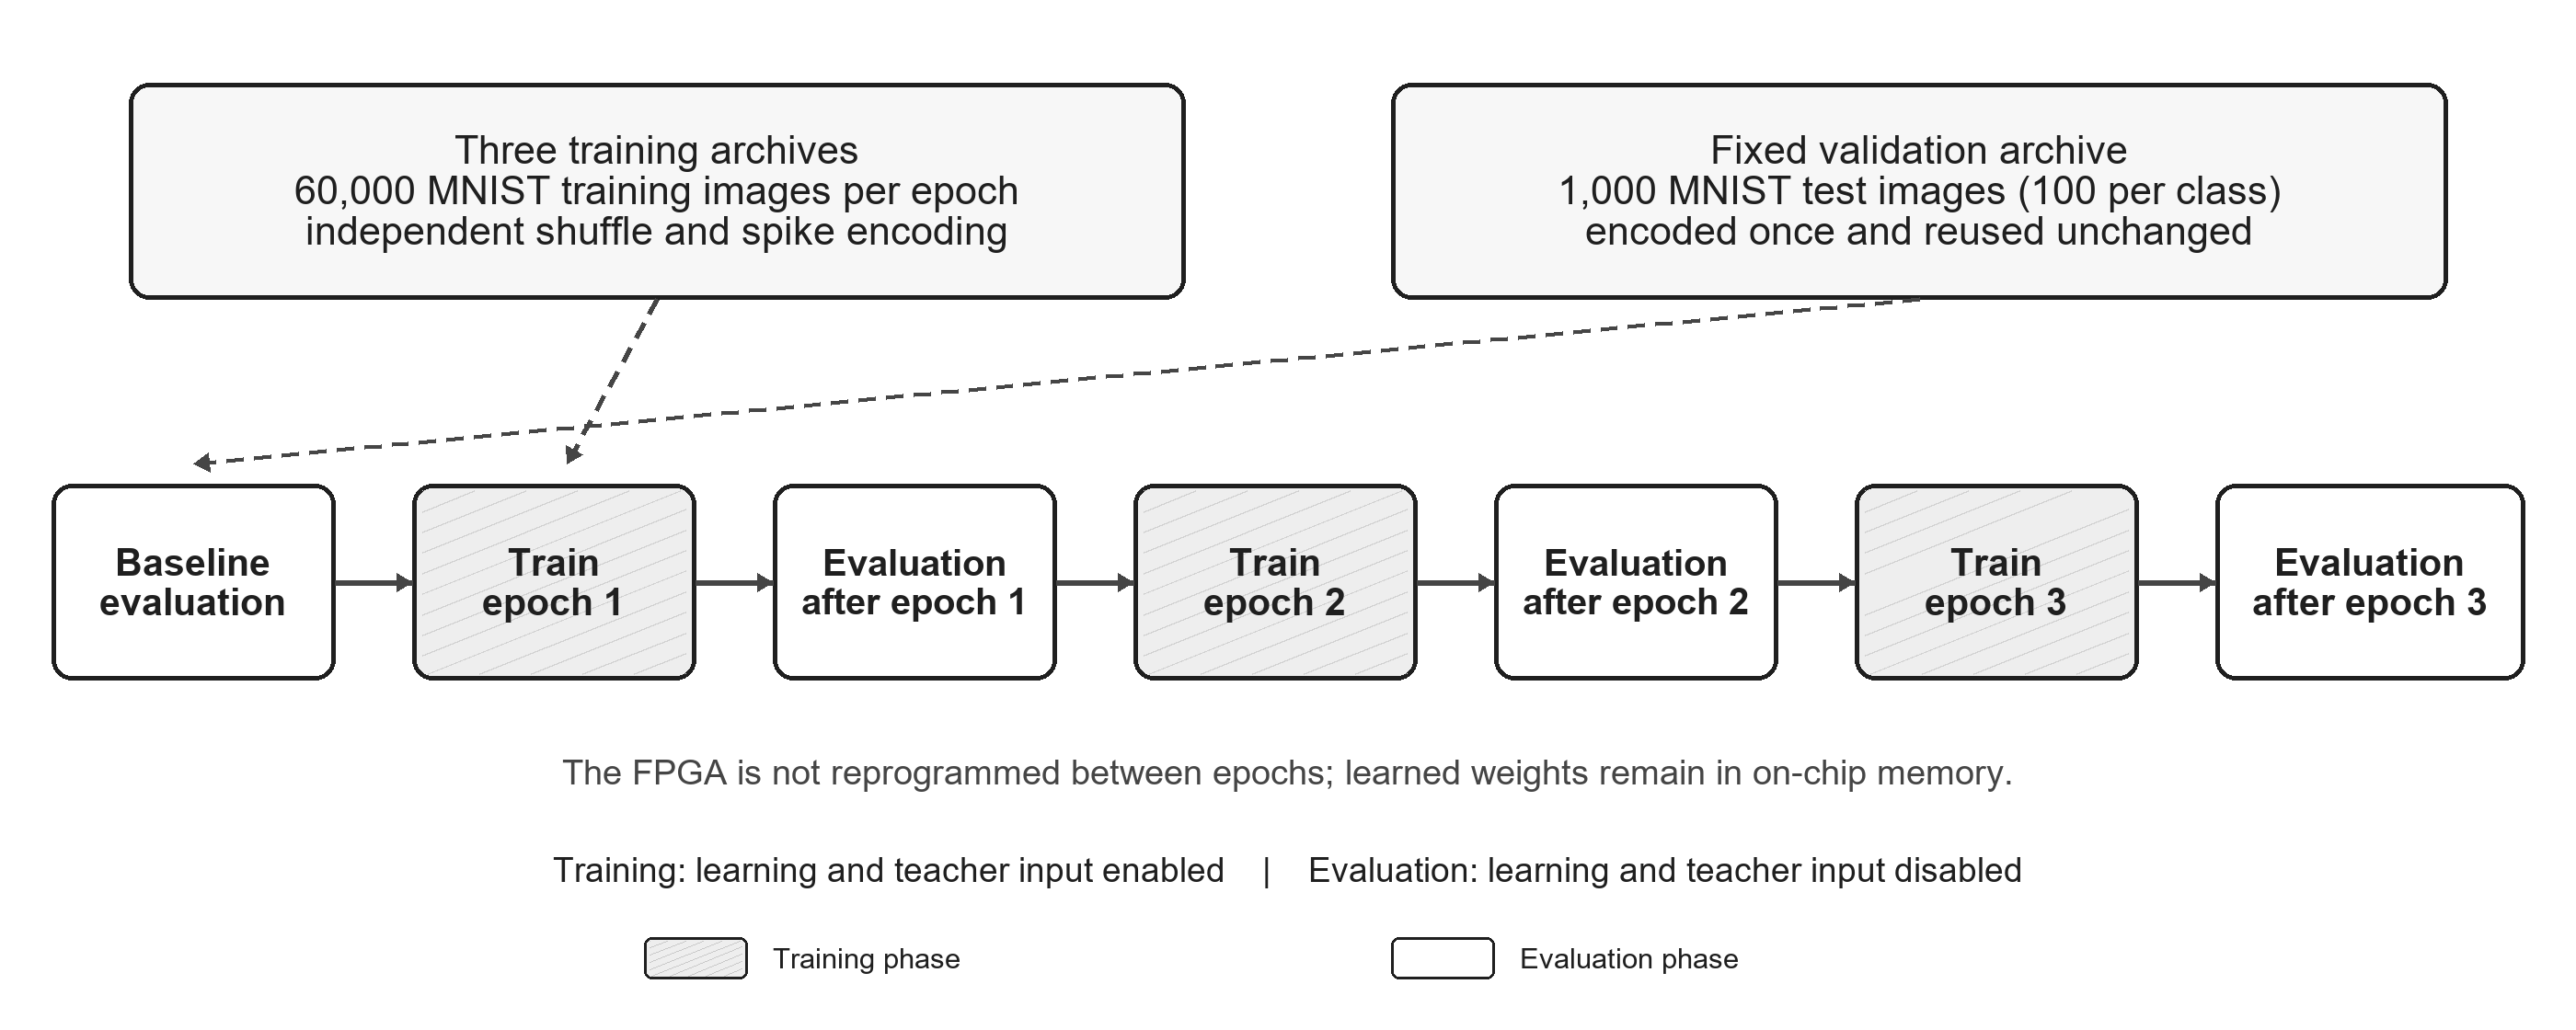
\includegraphics[width=\linewidth]{figures/evaluation_protocol.png}
	\caption{Training and Evaluation Protocol Used for the Three-Epoch Board Experiment}
	\label{fig:evaluation-protocol}
\end{figure}

Although the fixed images originate from the MNIST test partition, they are referred to as the \emph{validation set} in this chapter. Their results were inspected after each epoch and used to decide whether an additional epoch should be run. They therefore participated indirectly in the experimental decision process and do not constitute a fully independent final test set. This distinction limits the claims that can be made from the measured accuracy and is considered again in the discussion of the results.

\subsection{Evaluation Metrics}

Classification is derived from the ten output-neuron spike counts accumulated over one 100-step transaction. A sample is defined as \emph{silent} when all ten counts are zero. Silent samples require explicit treatment because applying a numerical argmax operation to an all-zero vector returns the first class even though the network produced no classification evidence. The primary metric is therefore strict accuracy, for which every silent sample is counted as incorrect.

Table \ref{tab:evaluation-metrics} defines the metrics reported in the following sections. Active-image accuracy is included as a diagnostic measure rather than as an alternative overall accuracy. Comparing it with strict accuracy reveals whether an improvement results from better class separation among responding samples or merely from a reduction in the number of silent samples. Total output spikes and the class-wise results provide complementary information about changes in network activity that would not be visible from accuracy alone.

\begin{table}[htbp]
	\centering
	\caption{Metrics Used to Evaluate the Online-Learning Experiment}
	\label{tab:evaluation-metrics}
	\small
	\begin{tabularx}{\linewidth}{@{}p{0.25\linewidth}X@{}}
		\toprule
		\textbf{Metric} & \textbf{Definition and purpose} \\
		\midrule
		Strict accuracy & Fraction of all validation images for which at least one output spike is produced and the neuron with the largest count corresponds to the true class. Silent images are counted as incorrect. \\
		Raw argmax accuracy & Fraction obtained by applying argmax directly to every count vector. This value is reported only as a diagnostic because an all-zero vector is assigned to class zero. \\
		Active-image accuracy & Accuracy calculated only over images that produce at least one output spike. It separates classification behaviour from the silent-output problem. \\
		Silent images & Number of images for which the sum of all ten output spike counts is zero. \\
		Total output spikes & Sum of all output-neuron spike counts over the complete validation set, used to characterize overall network activity. \\
		Per-class accuracy & Strict accuracy calculated separately for each digit class, used to identify class-dependent learning behaviour. \\
		\bottomrule
	\end{tabularx}
\end{table}

The reported learning curve is obtained from one continuous three-epoch hardware run. The independently encoded training archives introduce new spike realizations between epochs, whereas the fixed validation archive makes the four evaluation points directly comparable. However, the experiment does not include repeated training runs with different initial weights or parameter combinations. The results therefore demonstrate the behaviour and learning trend of the implemented configuration, but they do not provide an estimate of statistical variation across independent runs.

\section{Hardware Functional Validation}
\label{subsec:hardware-functional-validation}

Before evaluating classification performance, the deployed system was tested to establish that input data, control values, neural activity, and learning operations pass through the intended hardware path. These tests were performed on the PYNQ-Z1 using the final bitstream and its matching hardware-description file. They complement the RTL verification described in Section \ref{subsec:verification-infrastructure}: simulation checks internal timing and interface contracts, whereas the experiments in this section verify the integrated \gls{ps}, \gls{dma}, AXI, and accelerator system on the physical board.

\subsection{Board-Level Interface and Data-Path Tests}

The first checks were deliberately independent of MNIST classification accuracy. The overlay metadata was parsed before configuration to confirm that the memory-to-stream \gls{dma} and accelerator control interface appeared at the expected addresses. After configuration, the AXI4-Lite registers reported an idle accelerator, 100 configured time steps, and disabled learning and teacher modes. Configuration values written by the processor, including the target label, calcium-leak interval, bistability interval, and teacher current, were subsequently read back before an input transaction was started.

Two deterministic edge cases were then used to make failures directly observable. The zero-input test sent 100 time steps without an input spike. All steps were accepted, no stream or \gls{dma} error was reported, and the ten output-neuron counts remained zero. The dense-input test asserted all 784 valid input bits at every time step while keeping the unused upper bits of the final stream word at zero. The accelerator again accepted all 100 steps and reported 99 spikes for each output neuron, matching the behaviour observed in the corresponding RTL test. These cases exercise both inactivity and sustained input activity without depending on a trained classifier.

Table \ref{tab:board-functional-tests} summarizes the board-level checks. The fixed MNIST frames additionally verified that the packed 25-word representation could be transferred repeatedly and that the output counters could be read after each completed transaction. Finally, a 1,000-image supervised pilot completed without a transfer timeout, malformed-stream indication, or incomplete input count. Passing this test establishes continuous operation of the integrated data and control paths; it does not by itself establish that the resulting classifier is accurate.

\begin{table}[htbp]
	\centering
	\caption{Summary of Board-Level Functional Tests}
	\label{tab:board-functional-tests}
	\small
	\begin{tabularx}{\linewidth}{@{}p{0.20\linewidth}p{0.33\linewidth}X@{}}
		\toprule
		\textbf{Test} & \textbf{Applied check} & \textbf{Board observation} \\
		\midrule
		Overlay metadata & Parse the hardware description and inspect the instantiated IP blocks & The MM2S \gls{dma} and accelerator interfaces were present at their expected AXI addresses. \\
		Register interface & Read defaults, write the runtime parameters, and read them back & The accelerator reported 100 time steps and retained the programmed learning parameters. \\
		Zero-input stream & Transfer 2,500 zero-valued words with learning and teacher input disabled & All 100 steps were accepted, no interface error was set, and all ten output counts remained zero. \\
		Dense-input stream & Assert all 784 valid input bits in every time step & All 100 steps were accepted and every output neuron produced 99 spikes, consistent with RTL verification. \\
		MNIST inference & Transfer fixed, pre-encoded MNIST frames without learning & Each transaction completed with 100 accepted steps and reproducible output-count vectors. \\
		Teacher path & Train one label-7 sample with a Q9 teacher current of 128 & Only the selected output neuron responded to the teacher current, producing 27 spikes in the initial directed test. \\
		Continuous training & Process 1,000 supervised MNIST training images without reconfiguration & All images completed without a \gls{dma} timeout, stream error, or incomplete step count. \\
		\bottomrule
	\end{tabularx}
\end{table}

\subsection{Controlled Teacher-Signal and Weight-Update Test}

Activity observed while the teacher current is applied cannot alone prove that synaptic weights were updated. The additional current can directly cause the selected neuron to spike even if the new weight value is not stored. A controlled experiment was therefore performed to determine whether teacher-guided training leaves a persistent effect after both learning and teacher input have been disabled.

Figure \ref{fig:teacher-control-validation} shows the experiment and its observations. Both branches start by reloading the same bitstream and recording the initial inference counts of ten fixed MNIST samples. In the teacher-off control branch, sample zero, whose label is seven, is presented ten times with learning enabled but teacher input disabled. A subsequent inference pass over the ten samples produces exactly the same count vectors as the initial baseline. In the teacher-enabled branch, the initial weights are restored again and the same sample is presented for the same number of repetitions, this time with the label-7 teacher input enabled. During the following inference pass, five of the ten samples differ from the teacher-off result. Every observed difference is confined to output neuron seven, which is the neuron selected by the training label.

\begin{figure}[t]
	\centering
	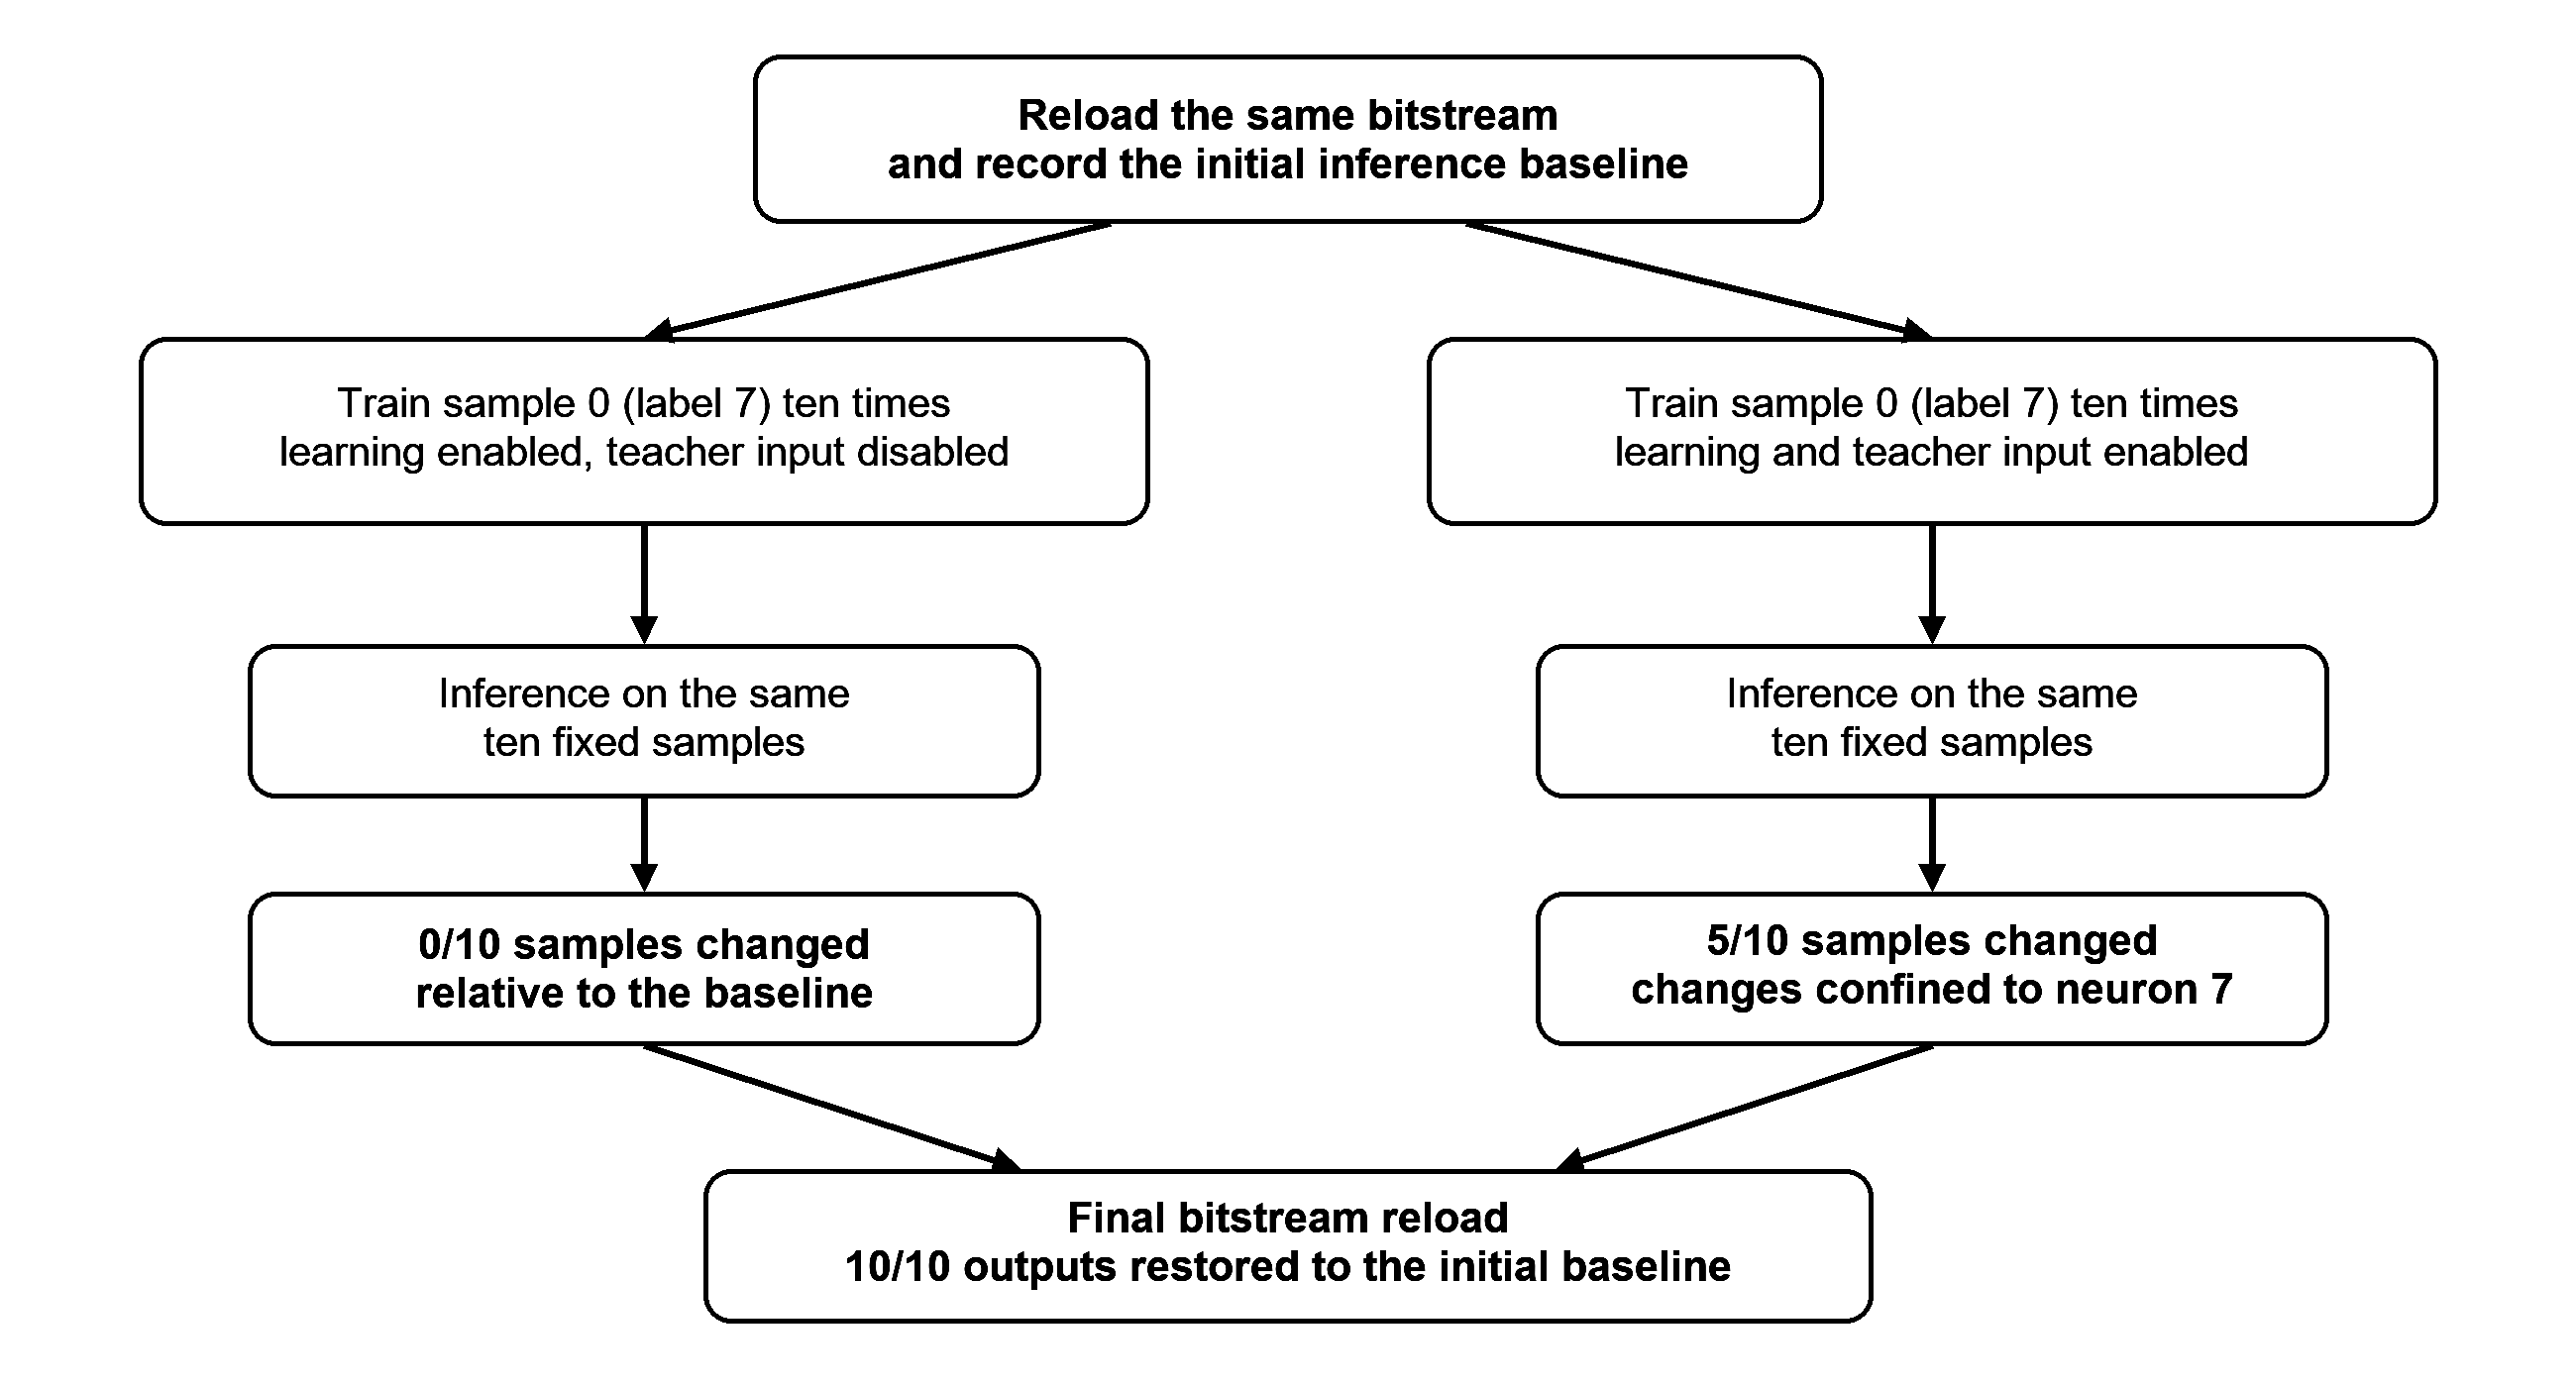
\includegraphics[width=\linewidth]{figures/teacher_control_validation.png}
	\caption{Teacher-Input Control Experiment and Observed Output Changes}
	\label{fig:teacher-control-validation}
\end{figure}

The inference transactions include a soft reset that clears the state required to start a new image while retaining the contents of the weight memory. The changed response therefore persists beyond the training transaction and cannot be explained only by the teacher current remaining active. As a final control, the bitstream is reloaded after the teacher-enabled experiment. All ten inference outputs then return to the recorded initial baseline. This confirms that the changed behaviour is associated with state stored in the configured accelerator and is discarded when the weight memory is reinitialized.

Taken together, the teacher-off branch, the target-specific change after teacher-enabled training, and restoration after bitstream reload provide behavioural evidence that the teacher path affects persistent synaptic updates. The experiment does not constitute a direct read-back of individual weight values because the implemented software interface exposes spike counts but not the complete excitatory memory. The conclusion is therefore limited to an observable and repeatable change in network behaviour consistent with the intended weight-update path.

\subsection{Software--Hardware Behavioural Comparison}

A final diagnostic test compares the deployed accelerator with the Spiker+ software model using the same stored input words. The first comparison exposed a difference in the initial conditions: the default software model initialized all excitatory weights with codes one and two, whereas the generated RTL initialization contains values across the complete 3-bit range. With these different weights, the software model remained silent for all ten samples while the hardware produced 176 output spikes. This result demonstrates why common input data alone are insufficient for a meaningful parity comparison.

The RTL initialization package was therefore decoded and loaded into the software model before repeating the baseline. Table \ref{tab:software-hardware-comparison} gives the resulting comparison and the measurements after both implementations processed the same 1,000-image training archive. With aligned initial weights, both models contain four silent samples and their total output activity differs by only 15 spikes before training. Five of the ten complete output-count vectors agree exactly. Following the training pilot, total activity decreases in both implementations, although the hardware exhibits a stronger reduction.

\begin{table}[htbp]
	\centering
	\caption{Software--Hardware Comparison on Ten Preserved MNIST Inputs}
	\label{tab:software-hardware-comparison}
	\small
	\begin{tabularx}{\linewidth}{@{}X >{\centering\arraybackslash}p{0.15\linewidth} >{\centering\arraybackslash}p{0.13\linewidth} >{\centering\arraybackslash}p{0.12\linewidth} >{\centering\arraybackslash}p{0.16\linewidth}@{}}
		\toprule
		\textbf{Comparison condition} & \textbf{Total spikes SW/HW} & \textbf{Silent SW/HW} & \textbf{Exact vectors} & \textbf{Absolute difference} \\
		\midrule
		Spiker+ default-weight baseline & 0/176 & 10/4 & 4/10 & 176 \\
		RTL-initialized baseline & 161/176 & 4/4 & 5/10 & 15 \\
		After the 1,000-image pilot & 42/20 & 4/6 & 4/10 & 26 \\
		\bottomrule
	\end{tabularx}
\end{table}

The post-training reduction is consequently not a hardware-only anomaly: the software model shows the same direction of change when it uses the preserved inputs and RTL-derived initial weights. Nevertheless, the two implementations are not bit-exact. The software model evaluates neuron dynamics with floating-point operations, whereas the accelerator uses fixed-point arithmetic, integer shifts, and an explicit multi-cycle schedule. These numerical and timing differences provide plausible sources for the remaining count deviations, but the present experiment does not isolate their individual contributions. The comparison therefore supports agreement at the behavioural-trend level rather than cycle-accurate equivalence.

Overall, the board tests verify the complete input and control path, isolate the effect of teacher-guided learning, and demonstrate that weight-dependent behaviour persists across transactions. These observations establish the functional basis required for the larger resource, performance, and three-epoch learning evaluations presented in the following sections.

\section{FPGA Implementation Results}
\label{subsec:fpga-implementation-results}

The final block design was synthesized, placed, and routed for the XC7Z020 device on the PYNQ-Z1. The results in this section are taken from the Vivado post-implementation reports and therefore describe the complete programmable-logic design, including the SNN accelerator IP and the supporting AXI, DMA, interconnect, and buffering logic introduced in Chapter~\ref{sec:implementation}. They should not be interpreted as measurements of the learning module in isolation.

\subsection{Resource Utilization}

Table~\ref{tab:implementation-resource-utilization} lists the implemented resource usage. LUTs are the most heavily used resource, with 5,056 of the 53,200 available LUTs occupied, corresponding to 9.50\%. The design uses 5,294 flip-flops, or 4.98\% of the device capacity. LUTRAM, BRAM, and global clock-buffer usage all remain below 3.2\%. The same percentages are visualized in Figure~\ref{fig:implementation-results-summary}.

\begin{table}[htbp]
	\centering
	\caption{Post-Implementation Resource Utilization on the XC7Z020}
	\label{tab:implementation-resource-utilization}
	\small
	\begin{tabular}{@{}lrrr@{}}
		\toprule
		\textbf{Resource} & \textbf{Used} & \textbf{Available} & \textbf{Utilization} \\
		\midrule
		LUT    & 5,056 & 53,200  & 9.50\% \\
		LUTRAM & 138   & 17,400  & 0.79\% \\
		FF     & 5,294 & 106,400 & 4.98\% \\
		BRAM   & 4     & 140     & 2.86\% \\
		BUFG   & 1     & 32      & 3.13\% \\
		\bottomrule
	\end{tabular}
\end{table}

The low overall percentages show that the integrated design fits comfortably on the selected device and leaves substantial programmable-logic capacity unused. This headroom could support additional control logic or a larger accelerator configuration. However, the percentages alone do not establish how far the network can be scaled: weight-memory capacity, memory bandwidth, and the sequential layer schedule must also be considered.

\begin{figure}[t]
	\centering
	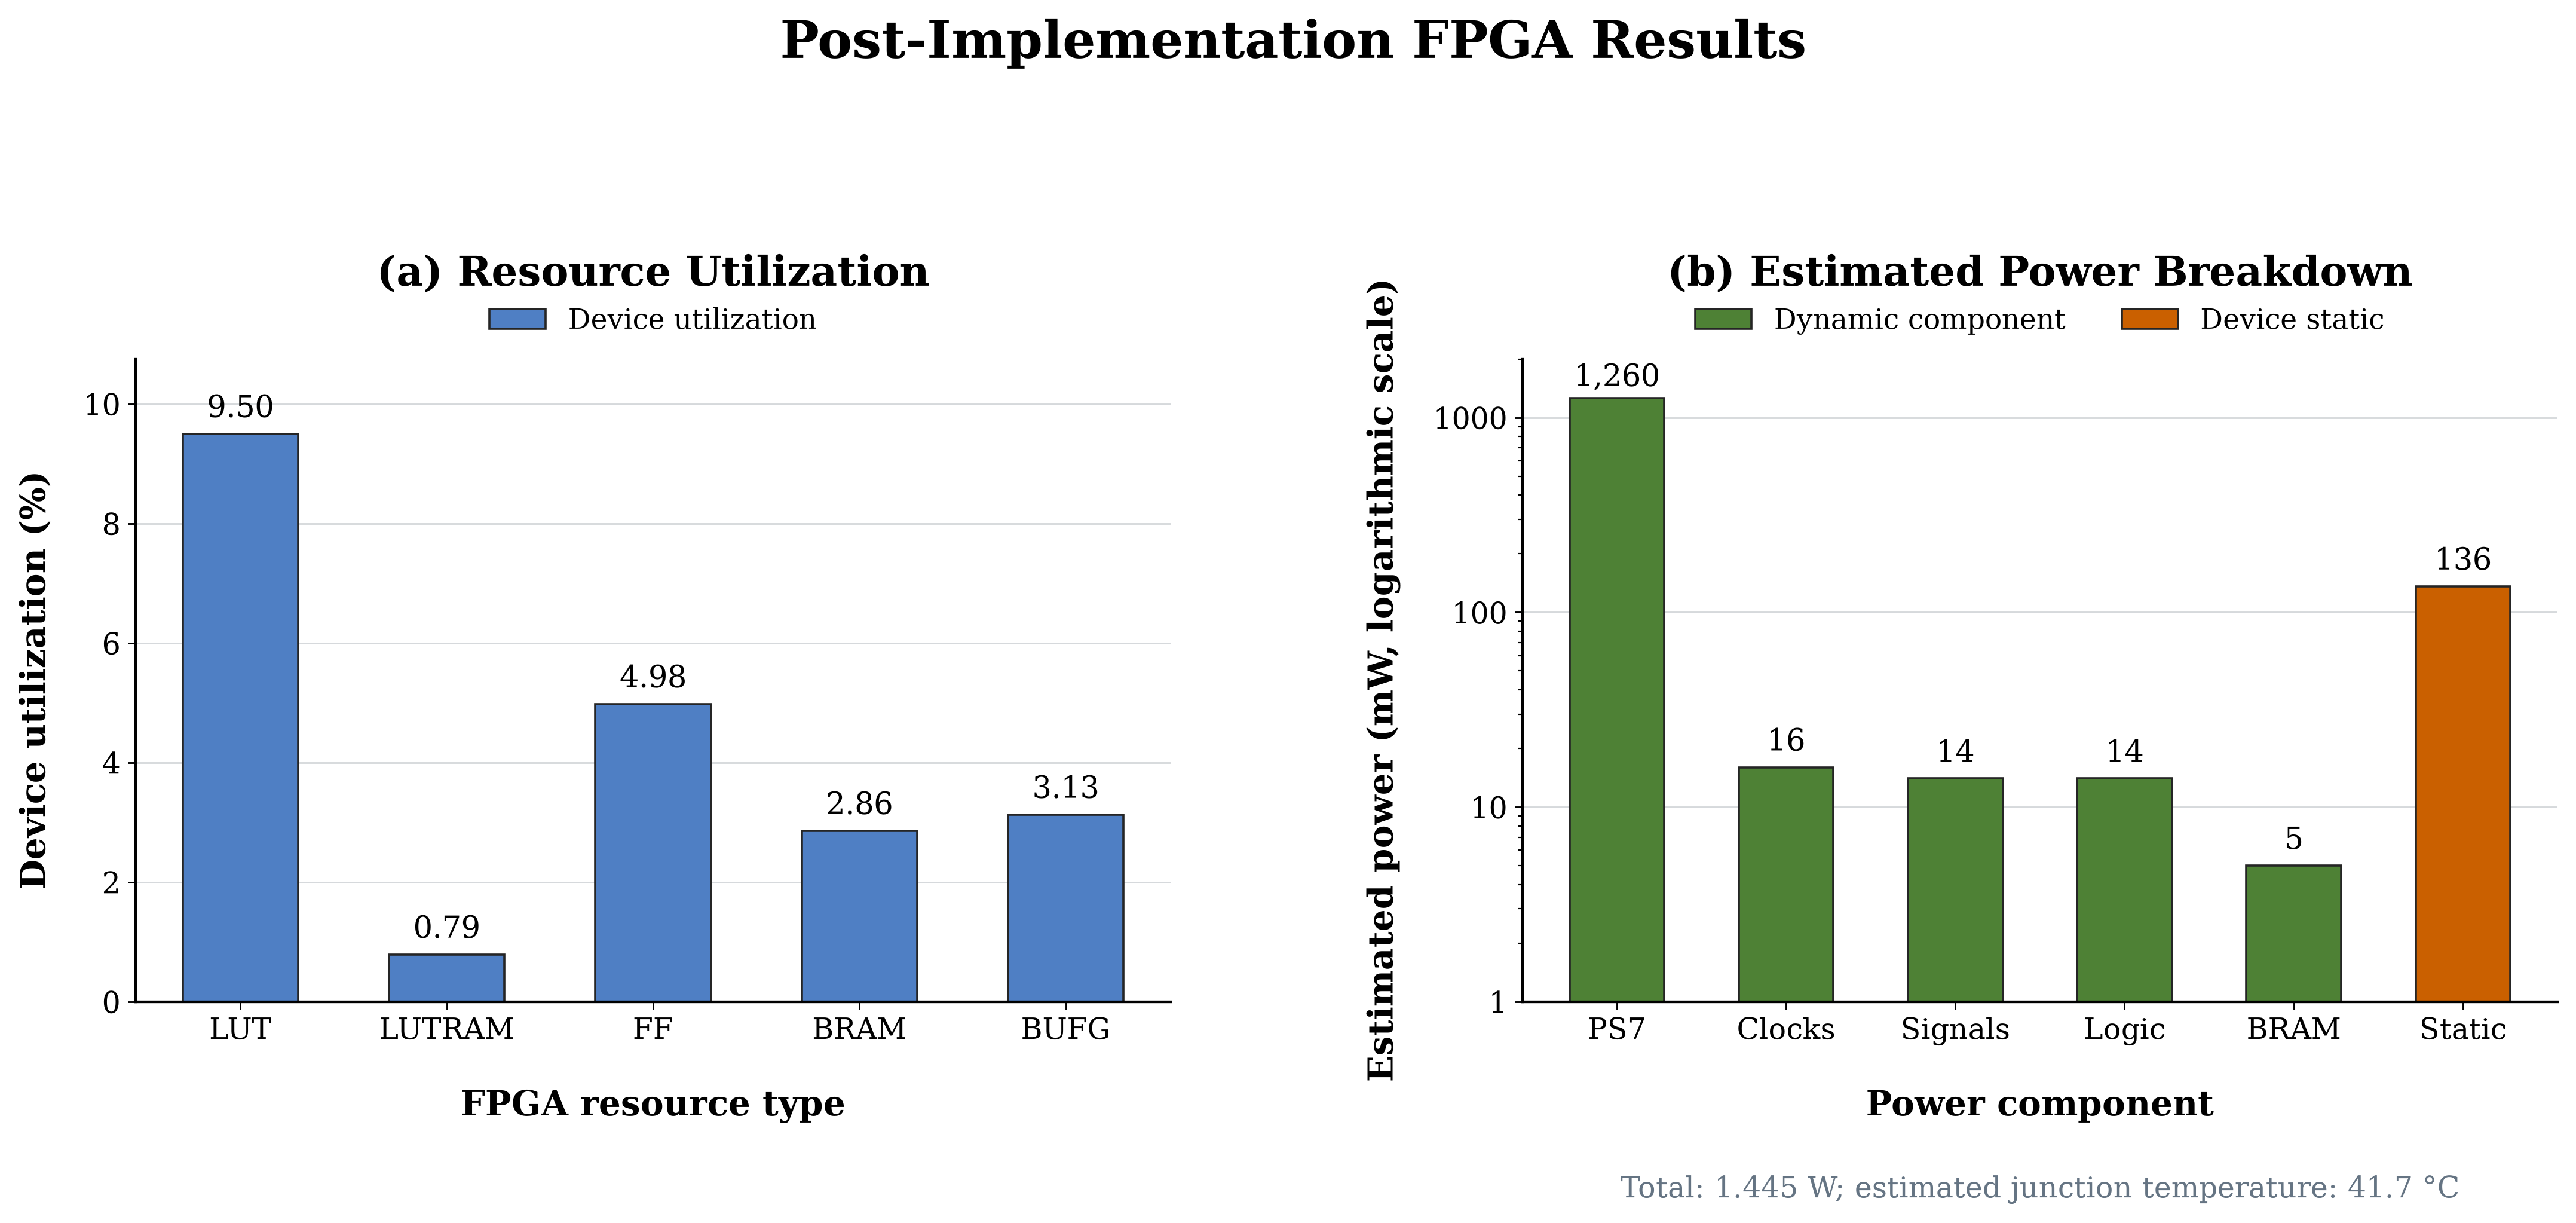
\includegraphics[width=\linewidth]{figures/implementation_results_summary.png}
	\caption{Post-Implementation Resource Utilization and Vivado Power Estimate for the Complete PYNQ-Z1 Design}
	\label{fig:implementation-results-summary}
\end{figure}

\subsection{Power and Thermal Estimate}

Table \ref{tab:implementation-power-summary} records the principal power and thermal values from the post-implementation report. Vivado estimates a total on-chip power of 1.445~W, divided into 1.309~W of dynamic power and 0.136~W of static power. Dynamic power therefore represents approximately 91\% of the estimate. Within the reported dynamic-power breakdown, the PS7 accounts for 1.260~W, or approximately 96.3\% of dynamic power. The reported contributions from clocks, signals, logic, and BRAM are 0.016~W, 0.014~W, 0.014~W, and 0.005~W, respectively. These four non-PS categories sum to approximately 49~mW, but they cover the complete programmable-logic design and cannot be attributed exclusively to the SNN accelerator.

\begin{table}[htbp]
	\centering
	\caption{Vivado Post-Implementation Power and Thermal Summary}
	\label{tab:implementation-power-summary}
	\small
	\begin{tabularx}{\linewidth}{@{}Xr@{}}
		\toprule
		\textbf{Reported quantity} & \textbf{Value} \\
		\midrule
		Total on-chip power & 1.445~W \\
		Dynamic power & 1.309~W (91\%) \\
		Static power & 0.136~W (9\%) \\
		Estimated junction temperature & 41.7~$^{\circ}$C \\
		Thermal margin & 43.3~$^{\circ}$C (3.6~W) \\
		Effective $\theta_{JA}$ & 11.5~$^{\circ}$C/W \\
		Power supplied to off-chip devices & 0~W \\
		Report confidence level & Medium \\
		\bottomrule
	\end{tabularx}
\end{table}

The estimated junction temperature is 41.7~$^{\circ}$C and the reported thermal margin is 43.3~$^{\circ}$C, indicating that the implemented configuration is not thermally constrained under the assumptions used by Vivado. Nevertheless, this result is an implementation estimate with a medium confidence level, not a measurement at the board power input. Moreover, it includes the processing system and the surrounding programmable-logic infrastructure. It is therefore unsuitable for a direct power-efficiency comparison with accelerator-only measurements reported by other neuromorphic processors unless a common measurement boundary and workload are established.

\subsection{Timing Closure}

Timing was evaluated for the implemented 100~MHz design. Table~\ref{tab:implementation-timing-summary} records the setup, hold, and pulse-width results. All three worst-case slack values are positive, the total negative slack is zero, and Vivado reports no failing endpoints. The smallest margin is the 0.012~ns worst hold slack, but it remains positive after implementation.

\begin{table}[htbp]
	\centering
	\caption{Post-Implementation Timing Summary at 100~MHz}
	\label{tab:implementation-timing-summary}
	\small
	\begin{tabularx}{\linewidth}{@{}X >{\centering\arraybackslash}p{0.16\linewidth} >{\centering\arraybackslash}p{0.20\linewidth} >{\centering\arraybackslash}p{0.16\linewidth} >{\centering\arraybackslash}p{0.12\linewidth}@{}}
		\toprule
		\textbf{Check} & \textbf{Worst slack} & \textbf{Total negative slack} & \textbf{Failing endpoints} & \textbf{Endpoints} \\
		\midrule
		Setup       & 0.117~ns & 0~ns & 0 & 16,053 \\
		Hold        & 0.012~ns & 0~ns & 0 & 16,053 \\
		Pulse width & 3.750~ns & 0~ns & 0 & 5,565 \\
		\bottomrule
	\end{tabularx}
\end{table}

These results demonstrate timing closure at the configured 100~MHz operating frequency for the final routed design. The positive setup slack should not be treated as a measured maximum clock frequency; determining such a limit would require progressively tightening the clock constraint and repeating implementation. Together with the resource and power reports, the timing results establish that the complete integrated system is implementable on the PYNQ-Z1 with substantial resource headroom and without reported timing violations at the selected operating point.

\section{Runtime Performance}
\label{subsec:runtime-performance}

Runtime was measured at the Python application boundary on the PYNQ-Z1. One image corresponds to a complete accelerator transaction containing 100 network time steps and 25 32-bit stream words per step. The reported wall times therefore include the interaction between the processing system and programmable logic rather than only the execution time of the SNN core.

\subsection{End-to-End Processing Time}

The fixed 1,000-image validation set was evaluated four times: once with the initial weights and once after each training epoch. Learning and teacher input were disabled during these measurements. As shown in Table~\ref{tab:runtime-performance}, all four evaluations took between 14.73~s and 14.80~s. Across the 4,000 inference transactions, the mean time was 14.76~ms per image, corresponding to an end-to-end throughput of approximately 67.8 images/s.

Each complete training epoch presented 60,000 images with learning and the label-dependent teacher input enabled. Epochs one, two, and three required 905.02~s, 910.33~s, and 905.42~s, respectively. Their corresponding throughputs are 66.30, 65.91, and 66.27 images/s. The three epochs processed 180,000 training images in a total of 2,720.77~s, or 45~min 20.77~s, yielding an aggregate throughput of 66.16 images/s. Figure~\ref{fig:runtime-performance} visualizes the measured consistency across the complete experiment.

\begin{table}[htbp]
	\centering
	\caption{Measured End-to-End Runtime on the PYNQ-Z1}
	\label{tab:runtime-performance}
	\small
	\begin{tabularx}{\linewidth}{@{}X >{\centering\arraybackslash}p{0.12\linewidth} >{\centering\arraybackslash}p{0.16\linewidth} >{\centering\arraybackslash}p{0.16\linewidth} >{\centering\arraybackslash}p{0.15\linewidth}@{}}
		\toprule
		\textbf{Measurement} & \textbf{Images} & \textbf{Wall time} & \textbf{Mean time/image} & \textbf{Throughput} \\
		\midrule
		Initial-weight evaluation & 1,000 & 14.80~s & 14.80~ms & 67.57 images/s \\
		Evaluation after epoch 1 & 1,000 & 14.73~s & 14.73~ms & 67.89 images/s \\
		Evaluation after epoch 2 & 1,000 & 14.73~s & 14.73~ms & 67.89 images/s \\
		Evaluation after epoch 3 & 1,000 & 14.76~s & 14.76~ms & 67.75 images/s \\
		Training epoch 1 & 60,000 & 905.02~s & 15.08~ms & 66.30 images/s \\
		Training epoch 2 & 60,000 & 910.33~s & 15.17~ms & 65.91 images/s \\
		Training epoch 3 & 60,000 & 905.42~s & 15.09~ms & 66.27 images/s \\
		\bottomrule
	\end{tabularx}
\end{table}

\begin{figure}[t]
	\centering
	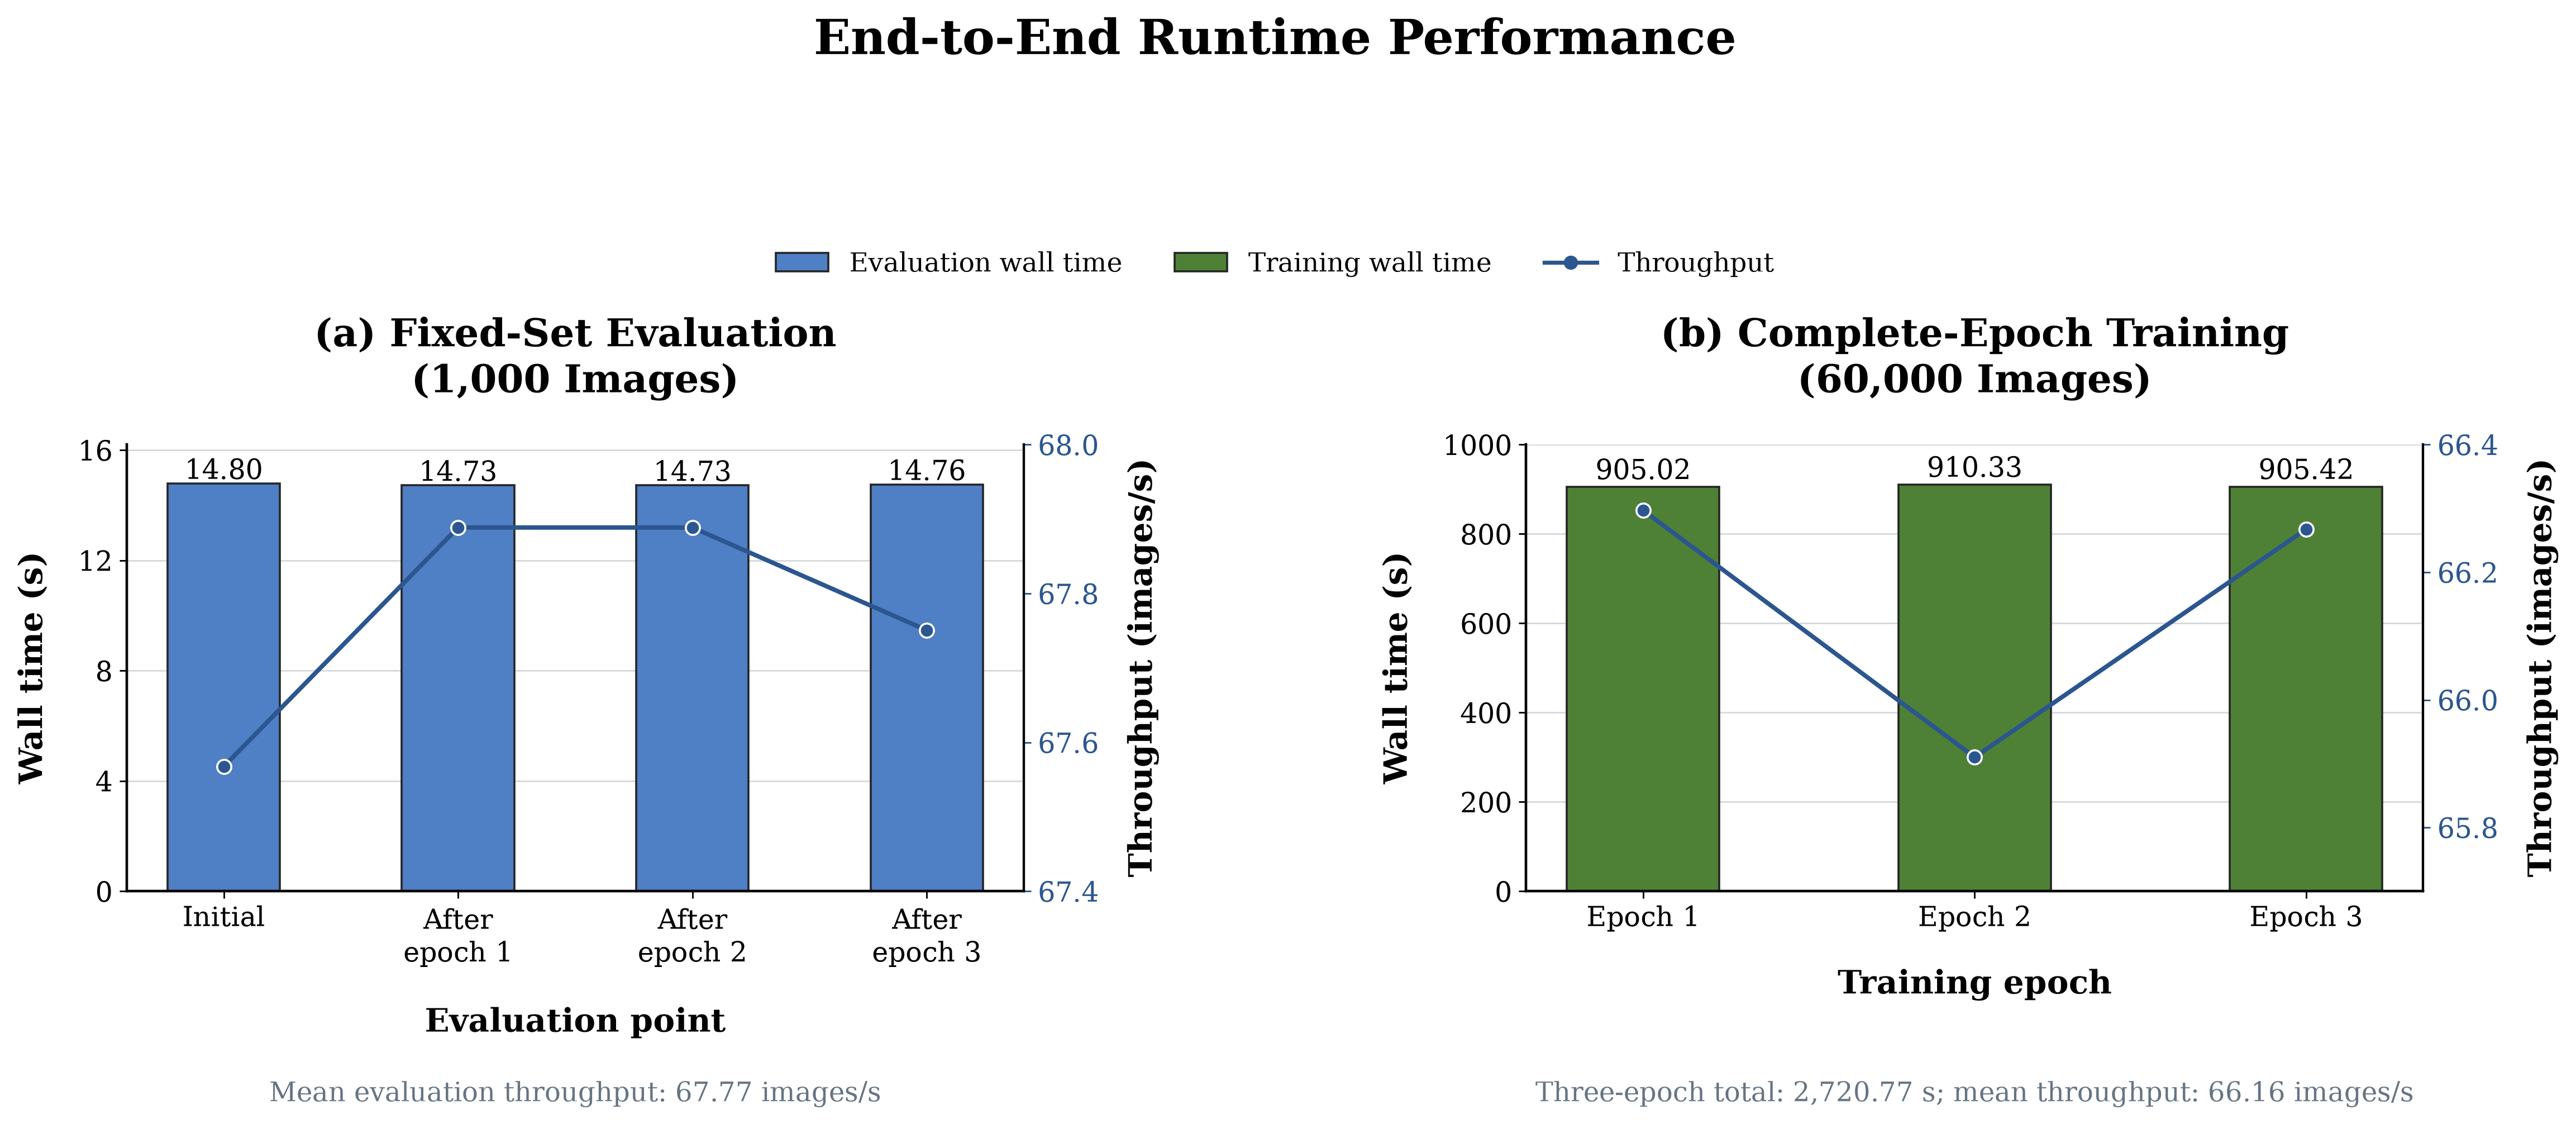
\includegraphics[width=\linewidth]{figures/runtime_performance.png}
	\caption{Measured End-to-End Runtime and Throughput for Evaluation and Training on the PYNQ-Z1}
	\label{fig:runtime-performance}
\end{figure}

The small variation between repeated validation measurements shows that the transaction time is stable as the synaptic weights and output activity change. Training is only slightly slower at the application level: the mean training time is 15.12~ms per image, compared with 14.76~ms for evaluation. This difference must not be interpreted as the isolated cost of the SDSP datapath, because the two measurements also differ in data-source handling and register configuration. It nevertheless demonstrates that enabling online learning does not prevent the system from maintaining a similar end-to-end transaction rate.

\subsection{Interpretation of the Benchmark}

The measured throughput is determined by the complete runtime sequence described in Chapter~\ref{sec:implementation}. For every image, the Python control function allocates a contiguous DMA buffer, copies and flushes 2,500 stream words, applies a soft reset, programs the required AXI4-Lite registers, starts the MM2S transfer, polls both the DMA and accelerator completion states, reads the ten output counters, and releases the buffer. The function also contains an explicit 10~ms delay after the soft reset. This delay alone establishes a substantial lower bound on the observed per-image wall time.

The evaluation data are loaded into processor memory before timing starts, so the values for the 1,000-image validation set exclude the initial NPZ-file loading time. In contrast, the epoch timer includes opening the training ZIP archive and reading and decompressing each 1,000-image shard as training proceeds. Despite this additional work, the epoch measurements remain close to the evaluation rate because both paths are dominated by per-image software control and synchronization.

Consequently, the reported 66--68 images/s characterize the implemented PYNQ application, including the Python, PS, AXI, DMA, and PL components. They are not a measurement of the maximum throughput of the SNN core alone. The design does not expose an internal cycle counter that isolates accelerator execution from DMA and processor overhead, and no batched command interface is implemented to amortize the per-image setup cost. A direct comparison between these values and a hardware-core frame rate reported by another accelerator would therefore use different measurement boundaries. The present benchmark instead establishes that the complete system operated continuously and repeatably throughout all 180,000 online-training transactions. Removing the fixed software delay, reusing DMA buffers, and batching multiple images per invocation are potential runtime optimizations, but they were not required for validating the online-learning architecture in this work.

\section{Online-Learning Results}
\label{subsec:online-learning-results}

The application-level learning behaviour was evaluated at four points during the continuous hardware experiment: before training and after each of the three complete epochs. At every evaluation point, learning and teacher input were disabled and the same 1,000 pre-encoded validation images were presented. The measurements therefore reflect the inference behaviour of the weight state produced by the preceding training, rather than the direct excitation caused by the teacher signal.

\subsection{Accuracy over Training Epochs}

Table~\ref{tab:online-learning-summary} summarizes the measured results. Strict accuracy, which counts every silent image as incorrect, increases from 5.9\% with the initialized weights to 32.0\% after the first epoch. This 26.1-percentage-point increase is the largest improvement observed in the experiment. The second and third epochs provide further increases of 4.3 and 3.3 percentage points, respectively, resulting in a strict accuracy of 39.6\% after three epochs. In absolute terms, the number of correctly classified validation images therefore increases from 59 to 396.

\begin{table}[htbp]
	\centering
	\caption{Learning Results on the Fixed 1,000-Image Validation Set}
	\label{tab:online-learning-summary}
	\small
	\begin{tabularx}{\linewidth}{@{}X >{\centering\arraybackslash}p{0.13\linewidth} >{\centering\arraybackslash}p{0.13\linewidth} >{\centering\arraybackslash}p{0.15\linewidth} >{\centering\arraybackslash}p{0.12\linewidth} >{\centering\arraybackslash}p{0.13\linewidth}@{}}
		\toprule
		\textbf{Training state} & \textbf{Strict accuracy} & \textbf{Raw argmax accuracy} & \textbf{Active-image accuracy} & \textbf{Silent images} & \textbf{Output spikes} \\
		\midrule
		Initial weights & 5.9\% & 6.3\% & 7.61\% & 225 & 26,653 \\
		After epoch 1 & 32.0\% & 33.0\% & 51.61\% & 380 & 4,116 \\
		After epoch 2 & 36.3\% & 38.3\% & 50.56\% & 282 & 6,486 \\
		After epoch 3 & 39.6\% & 40.2\% & 50.45\% & 215 & 8,522 \\
		\bottomrule
	\end{tabularx}
\end{table}

The raw argmax result is consistently higher than strict accuracy because an all-zero output vector is assigned to class zero by the software argmax operation. This difference is a measurement artifact rather than additional classification evidence, and strict accuracy is consequently used as the primary result. The active-image accuracy rises sharply from 7.61\% to 51.61\% during the first epoch but remains close to 50.5\% during epochs two and three. Figure~\ref{fig:learning-results-overview} shows both the accuracy metrics and the accompanying change in output activity.

\begin{figure}[t]
	\centering
	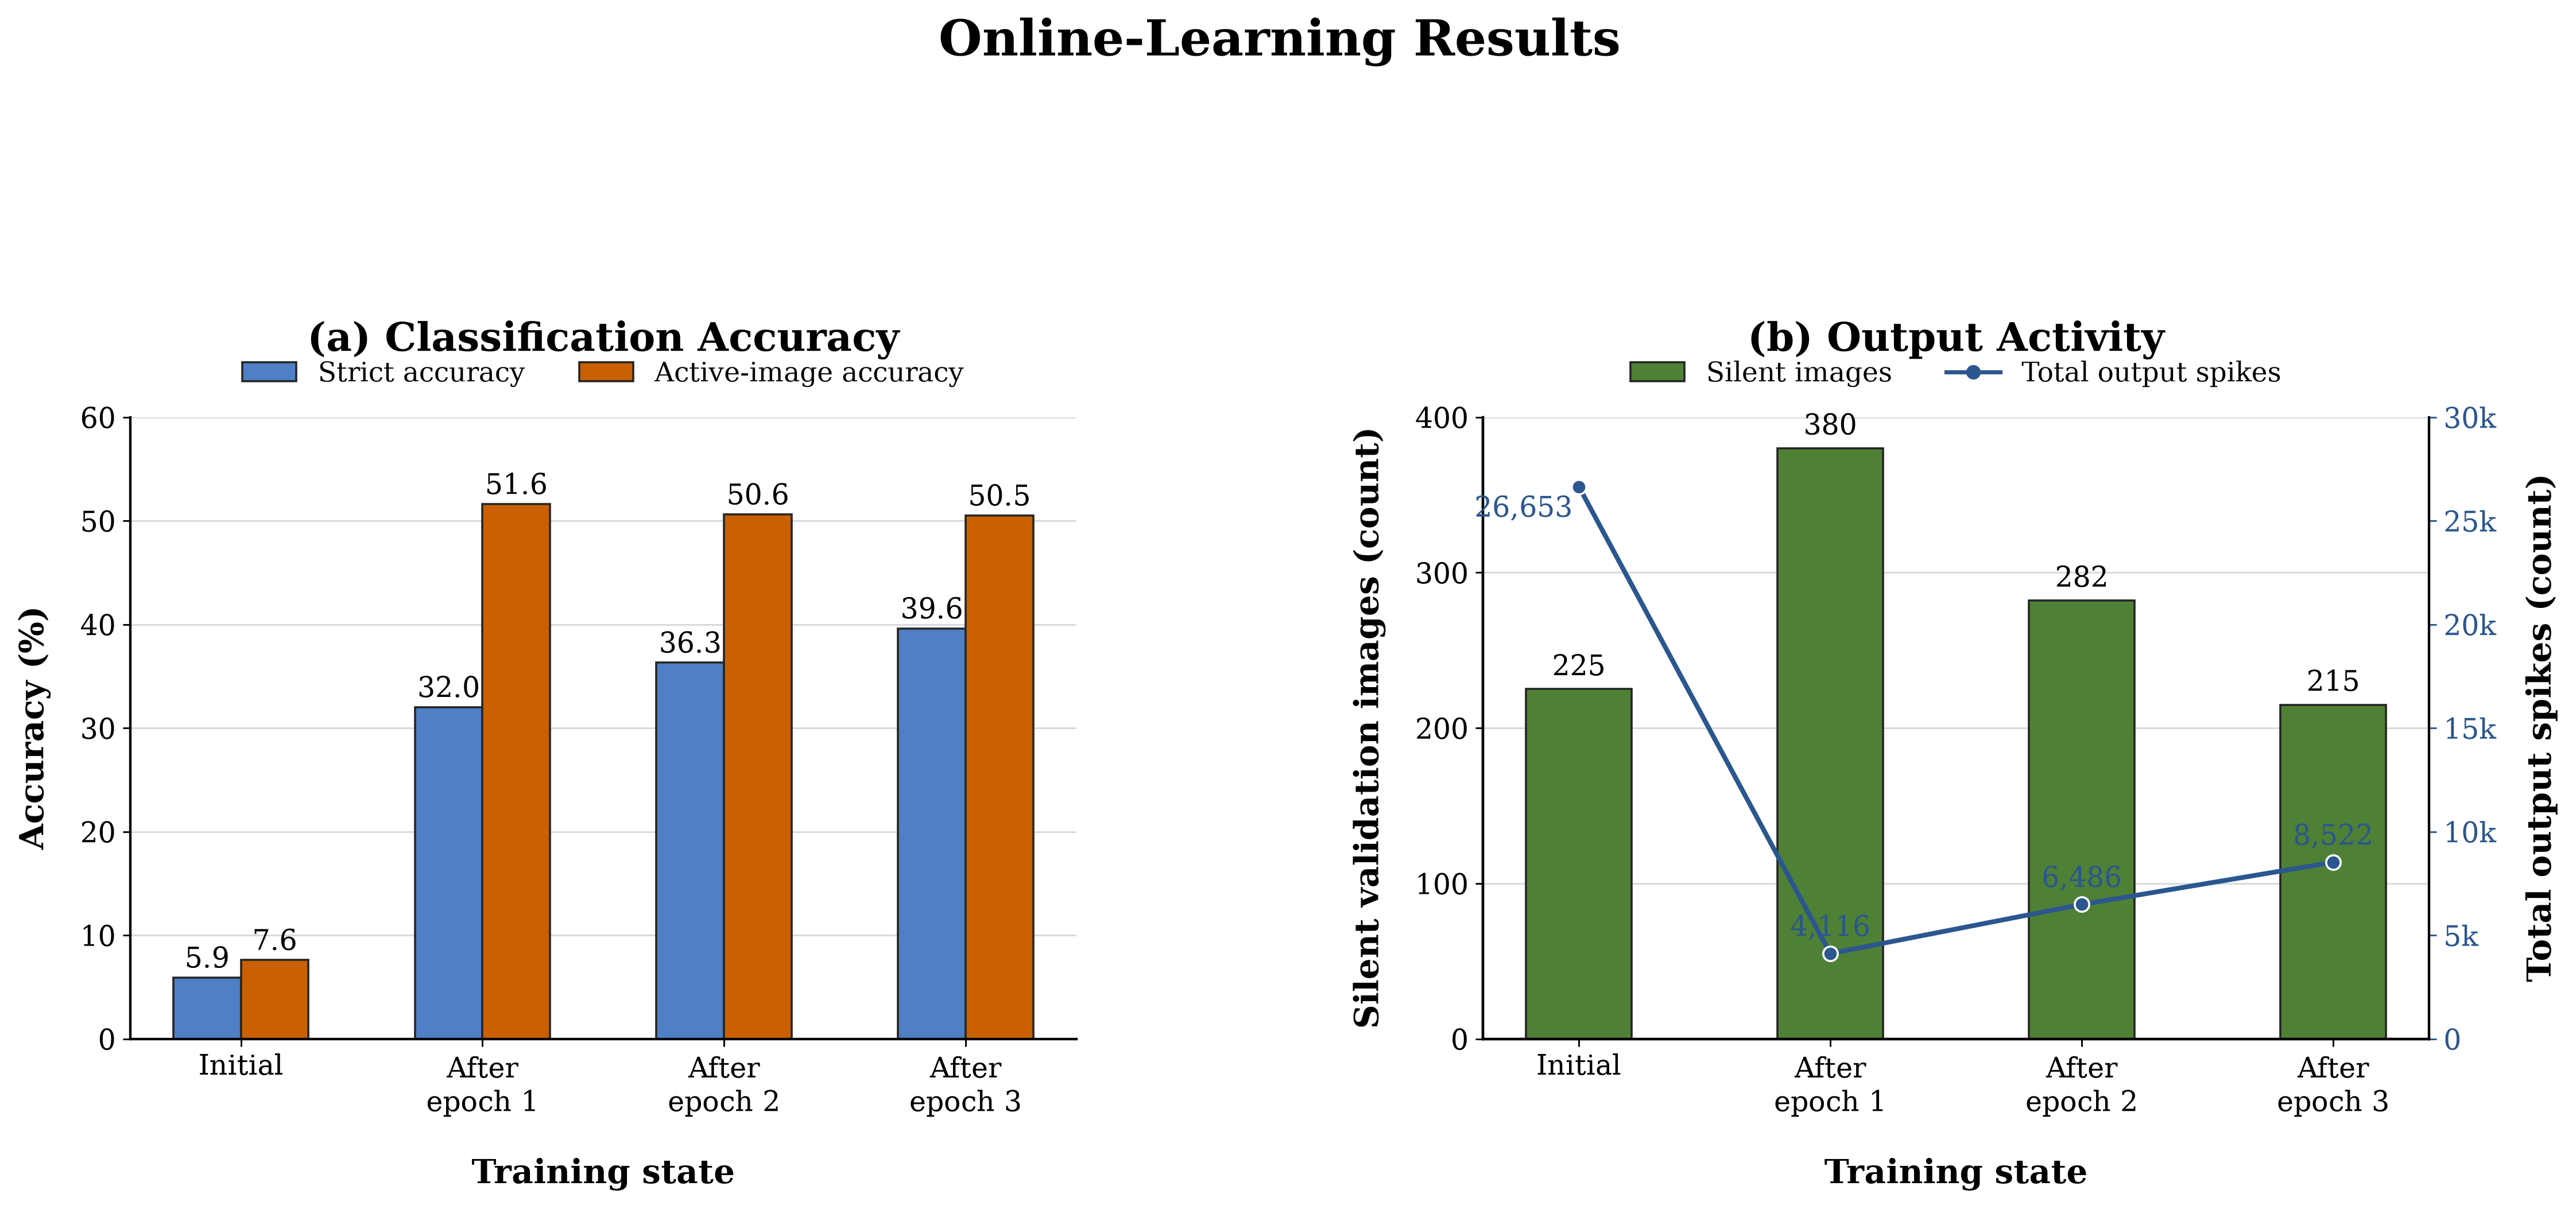
\includegraphics[width=\linewidth]{figures/learning_results_overview.png}
	\caption{Strict and Active-Image Accuracy Together with Output Activity over Three Hardware Training Epochs}
	\label{fig:learning-results-overview}
\end{figure}

The monotonically increasing strict accuracy demonstrates a positive learning trend for the tested configuration. However, the smaller gains in the later epochs and the nearly constant active-image accuracy do not establish convergence. Only one continuous training run was performed, no systematic parameter sweep was carried out, and the accuracy was still increasing after epoch three. The value of 39.6\% should therefore be interpreted as an intermediate validation result after a limited training duration, not as the maximum achievable accuracy of the architecture.

\subsection{Output Activity and Silent Samples}

The activity measurements provide important context for the accuracy curve. The initialized network produces 26,653 output spikes across the validation set, but its strict accuracy is only 5.9\%. High initial activity therefore does not correspond to useful class separation. After the first epoch, the total activity falls to 4,116 spikes and the number of silent images increases from 225 to 380. At the same time, active-image accuracy reaches 51.61\%. The first epoch thus suppresses a large amount of non-discriminative activity while substantially improving the predictions made for images that still produce a response.

During the second and third epochs, output activity partially recovers to 6,486 and 8,522 spikes, while the number of silent images decreases to 282 and then 215. Since active-image accuracy changes only from 51.61\% to 50.45\% across the three trained states, the later increase in strict accuracy is mainly caused by improved response coverage: more validation images produce at least one output spike and can therefore receive a meaningful prediction. The third epoch illustrates this effect most clearly. Strict accuracy rises by 3.3 percentage points from epoch two to epoch three, whereas active-image accuracy decreases slightly from 50.56\% to 50.45\%.

These observations show why output activity must be reported together with accuracy. A reduction in total spikes can remove unwanted responses, but excessive suppression creates silent inputs; conversely, increased activity is beneficial only if the resulting spikes support the correct class. The measured trajectory reflects both effects and cannot be described adequately by a single accuracy value.

\subsection{Per-Class Performance}

Figure~\ref{fig:per-class-learning-accuracy} presents the strict accuracy of each digit class. Because the validation set contains exactly 100 images from every class, each displayed percentage also equals the number of correct images for that class. The results reveal considerable class-dependent variation that is hidden by the aggregate accuracy.

\begin{figure}[t]
	\centering
	\makebox[\linewidth][c]{%
		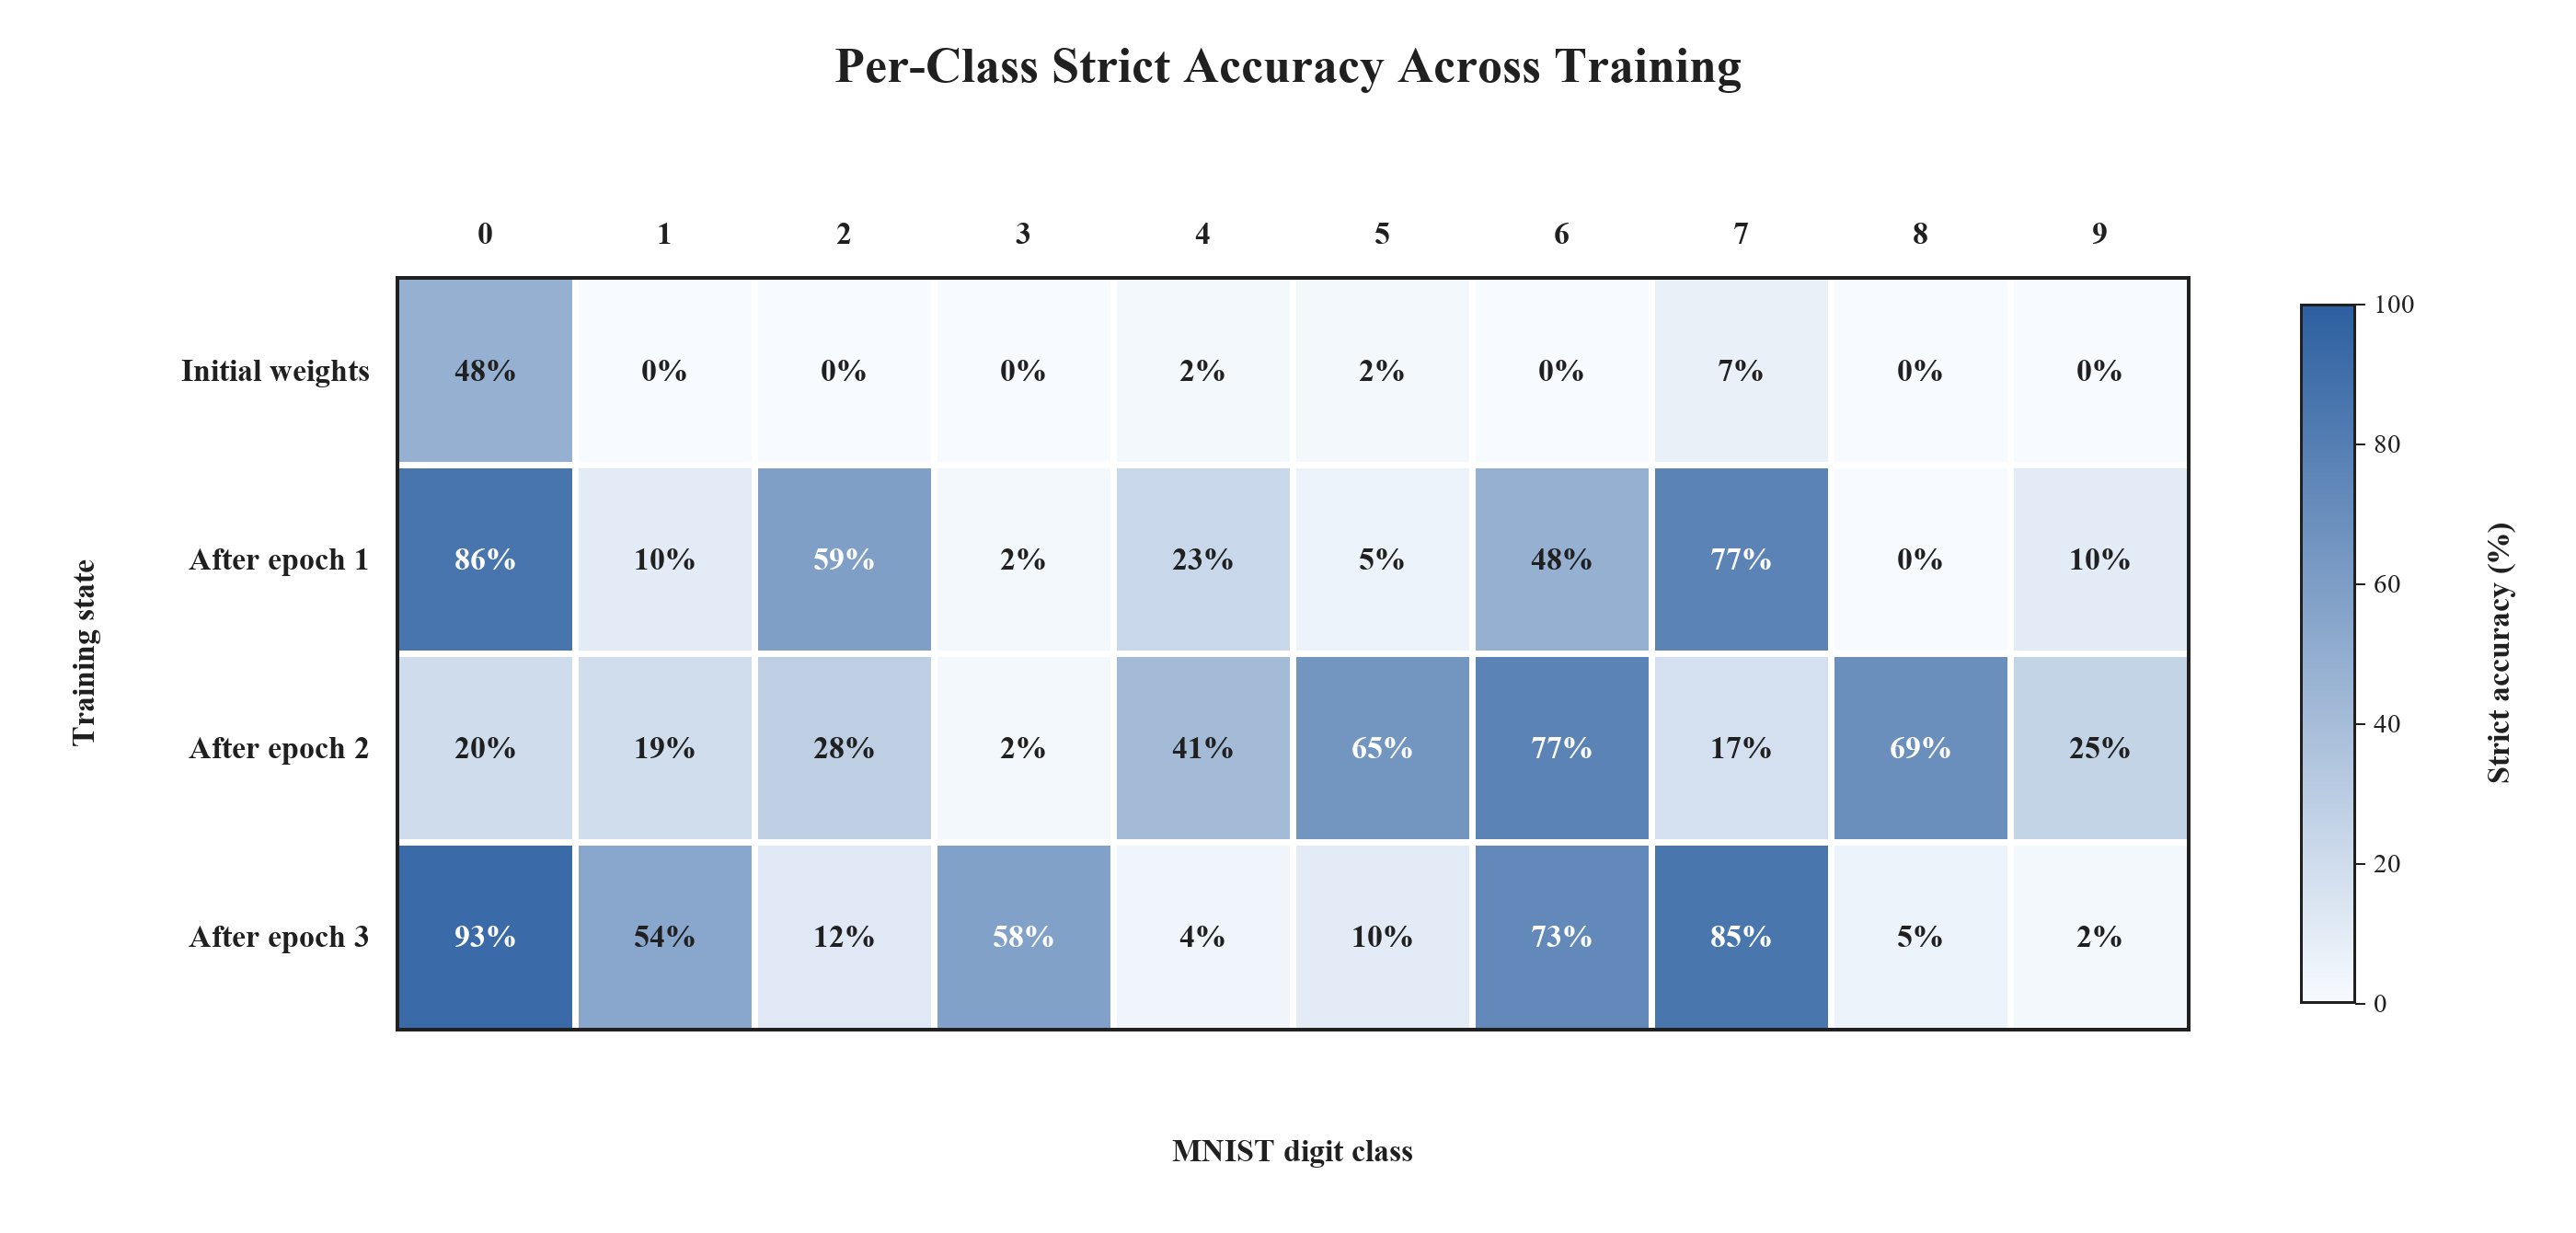
\includegraphics[width=1.06\linewidth]{figures/per_class_learning_accuracy.png}%
	}
	\caption{Per-Class Strict Accuracy on the Fixed Class-Balanced Validation Set}
	\label{fig:per-class-learning-accuracy}
\end{figure}

After the first epoch, classes zero, seven, two, and six achieve the strongest results, with accuracies of 86\%, 77\%, 59\%, and 48\%, respectively. The distribution changes substantially after the second epoch: classes six, eight, and five reach 77\%, 69\%, and 65\%, while the accuracy of classes zero and seven falls to 20\% and 17\%. After the third epoch, classes zero and seven recover to 93\% and 85\%, and classes six, three, and one reach 73\%, 58\%, and 54\%. In contrast, the final accuracies for classes four, eight, and nine are only 4\%, 5\%, and 2\%.

The weak final classes do not all fail in the same manner. For example, 48 of the class-four images and 32 of the class-nine images are silent after epoch three, whereas only 11 class-eight images are silent. The low class-eight accuracy is therefore primarily associated with incorrect competition among active outputs rather than a lack of output activity. This distinction suggests that reducing the overall number of silent samples alone would not remove the observed class imbalance.

The large changes between epochs show that individual class responses had not stabilized within the three-epoch experiment. They may be influenced by the local SDSP dynamics, the discrete 3-bit weight states, the initial weight distribution, and the fixed teacher and calcium parameters, but the present measurements do not isolate the contribution of each factor. The per-class results therefore support the same conclusion as the aggregate curve: the FPGA implements effective online adaptation, but the selected network and training configuration require further epochs and parameter investigation before their classification performance can be considered optimized.

\section{Comparison with SDSP-Based Related Work}
\label{subsec:comparison-with-related-work}

The broad literature review in Table~\ref{tab:related-work-comparison} includes both \gls{sdsp}- and \gls{stdp}-based systems. For evaluation of the implemented learning architecture, the comparison is narrowed to ODIN, MorphIC, the multiplier-less \gls{sdsp} circuit of Asgari et al., and TEDOP \cite{Frenkel2019ODIN,Frenkel2019MorphIC,Asgari2020SDSP,Shi2022TEDOP}. These works all implement \gls{sdsp} or a directly derived stochastic variant, but they differ substantially in technology, neuron dynamics, topology, input preparation, and evaluation scope. The values below therefore position the present design within this family of approaches; they do not form a normalized ranking.

\subsection{Rationale for the Single-Layer Network}

The 784--10 topology used in this work was selected deliberately to match the input and output dimensions of the MNIST network evaluated by TEDOP \cite{Shi2022TEDOP}. Using no hidden layer keeps the principal comparison focused on the integration of online synaptic plasticity into an event-driven hardware datapath. Introducing a hidden layer could improve the representational capacity of the classifier, but it would also change the synaptic memory, processing schedule, and learning dynamics. The resulting system would consequently be less useful as a structural reference to TEDOP.

This choice should not be interpreted as an assertion that a single-layer network is optimal for MNIST. Its purpose is methodological: it provides a compact and reproducible configuration in which weight write-back, teacher guidance, and persistent online adaptation can be evaluated on the \gls{fpga}. ODIN also evaluates a single-layer ten-class classifier, but its input is reduced to 256 values; MorphIC and the circuit of Asgari et al. do not provide an equivalent 784--10 online-learning experiment. TEDOP is therefore the closest topological reference, even though it is not algorithmically identical to the present network.

\subsection{Algorithmic Context}

Among the selected systems, ODIN is the closest reference for the learning rule itself. Its teacher-supervised \gls{sdsp} decision uses a presynaptic event together with the postsynaptic membrane potential and calcium state, as does the implementation developed in this thesis \cite{Frenkel2019ODIN}. However, ODIN embeds the rule in a time-multiplexed custom processor with configurable neuron dynamics and a $(3+1)$-bit synapse format. MorphIC instead adapts \gls{sdsp} to binary weights by applying eligible transitions stochastically. Its online demonstration is an eight-pattern task, whereas its 97.8\% MNIST result uses weights trained offline \cite{Frenkel2019MorphIC}. The design by Asgari et al. uses a 32-bit fixed-point state and demonstrates potentiation and depression in a two-neuron, one-synapse network, but it does not report a classification experiment \cite{Asgari2020SDSP}.

TEDOP uses a 16-bit Temporal-Integrate neuron derived from the integrate-and-fire model by removing its firing mechanism \cite{Shi2022TEDOP}. Its membrane potential is updated only when an input event is received. Each event contributes the corresponding excitatory weight minus a constant inhibitory term, while an additional teacher term may be applied during training. The neuron has no firing threshold, produces no output spikes, and performs no firing reset. After all events belonging to a sample have been processed, the decision unit selects the neuron with the largest final membrane potential.

The associated S4DSP rule also differs from the calcium-dependent \gls{sdsp} implementation used in this thesis. TEDOP evaluates the membrane potential against three update thresholds and probabilistically increments or decrements the active synaptic weight. The random decision is generated by a linear-feedback shift register. By exploiting an approximate relationship between the accumulated Temporal-Integrate potential and the output-spike count of a reference integrate-and-fire neuron, S4DSP removes the separate calcium state used by conventional \gls{sdsp}. This co-simplification of the neuron and learning models is central to TEDOP's small hardware footprint \cite{Shi2022TEDOP}.

In contrast, the present accelerator retains the modified subtractive-reset \gls{lif} neurons generated by Spiker+, including output-spike generation, reset behaviour, and recurrent output inhibition. Classification is based on the ten output spike counts rather than on final membrane potentials. The implemented \gls{sdsp} rule stores a calcium counter for each postsynaptic neuron and combines its state with the membrane-potential condition to form the \texttt{up} and \texttt{down} decisions. The selected 3-bit weight is then changed by one discrete level with saturation. Consequently, the equal 784--10 dimensions provide a useful topological reference to TEDOP, but they do not make the two classifiers equivalent.

\subsection{Quantitative Comparison and Measurement Boundaries}

Table~\ref{tab:sdsp-evaluation-comparison} repeats the \gls{sdsp}-based references from Chapter~\ref{sec:related_work}, adds the present implementation, and includes the quantitative implementation data that are relevant only after the measurement methodology of this chapter has been established. Values for the present work are those reported in the preceding sections.

% Quantitative comparison for Section 6.6.
\begin{table}[p]
	\centering
	\caption{Comparison with SDSP-Based Related Work}
	\label{tab:sdsp-evaluation-comparison}
	\begingroup
	\scriptsize
	\sloppy
	\setlength{\tabcolsep}{1.8pt}
	\renewcommand{\arraystretch}{1.03}
	\begin{tabularx}{\textwidth}{@{}
		>{\raggedright\arraybackslash}p{1.45cm}
		*{5}{>{\raggedright\arraybackslash}X}@{}}
		\toprule
		\textbf{Metric} &
		\shortstack[l]{\textbf{ODIN}\\\cite{Frenkel2019ODIN}} &
		\shortstack[l]{\textbf{MorphIC}\\\cite{Frenkel2019MorphIC}} &
		\shortstack[l]{\textbf{Asgari et al.}\\\cite{Asgari2020SDSP}} &
		\shortstack[l]{\textbf{TEDOP}\\\cite{Shi2022TEDOP}} &
		\textbf{This work} \\
		\midrule

		\textbf{Platform} &
		28-nm ASIC &
		65-nm ASIC &
		Spartan-6 XC6SLX45 FPGA &
		Zynq-7010 FPGA &
		PYNQ-Z1, XC7Z020 FPGA \\

		\textbf{Evaluated boundary} &
		Complete neuromorphic chip &
		Complete four-core chip &
		Two-neuron, one-synapse test network &
		Specialized learning core &
		Complete PL design; PS included in power estimate \\

		\textbf{Topology} &
		256--10 MNIST classifier &
		Four-core hierarchy; eight-class online benchmark &
		1--1 test network &
		784--10 MNIST classifier &
		784--10 MNIST classifier \\

		\textbf{Neuron and decision} &
		Configurable LIF or phenomenological neuron; rate or first-spike decision &
		LIF neurons; task-dependent output aggregation &
		LIF neurons with a calcium estimator &
		16-bit Temporal-Integrate; final-potential argmax &
		Modified subtractive-reset LIF; output-spike-count argmax \\

		\textbf{Learning and weights} &
		Teacher-supervised SDSP; 3-bit weight plus mapping bit &
		Stochastic SDSP; binary weights &
		Multiplier-less SDSP; 32-bit fixed point &
		Stochastic S4DSP; 8-bit weights &
		Calcium- and membrane-dependent SDSP; 3-bit weights \\

		\textbf{Input and training protocol} &
		28$\times$28 to 16$\times$16, deskewed and soft-thresholded; 6k samples presented once &
		Online eight-pattern task; reported MNIST result uses offline training &
		Synthetic spike trains; no classifier training &
		784-pixel rate code; 200 steps; epoch count N/R &
		784-pixel rate code; 100 steps; three 60k-sample epochs \\

		\textbf{Clock} &
		75~MHz &
		55~MHz &
		131~MHz &
		250~MHz &
		100~MHz \\

		\textbf{Reported implementation} &
		0.086\,$\mathrm{mm}^{2}$; 256 neurons; 64k synapses &
		2.86\,$\mathrm{mm}^{2}$; ${\sim}$2k neurons; ${>}$2M synapses &
		450 LUTs; 249 registers &
		952 LUTs; 741 FFs; 4 BRAMs; 0 DSPs &
		5,056 LUTs; 5,294 FFs; 4 BRAMs \\

		\textbf{Power or energy} &
		12.7~pJ/SOP; 15~nJ/inference at 0.55~V &
		51~pJ/SOP; 21.8~$\mu$J/classification &
		N/R &
		39~mW; 3.46~$\mu$J/training image; 3.32~$\mu$J/inference image &
		1.445~W whole-device estimate; isolated energy N/R \\

		\textbf{Online-learning result} &
		85.0\% rate; 84.5\% rank order on full 10k MNIST test set &
		800/800 pattern samples; 97.8\% MNIST is offline &
		LTP and LTD verified; no classification result &
		90.4\% MNIST test accuracy &
		39.6\% strict accuracy on fixed 1k validation set after epoch three \\

		\textbf{Reported rate} &
		N/R &
		N/R &
		N/A &
		11,268 training; 11,749 inference frames/s &
		66.16 training; ${\sim}$67.8 inference images/s end-to-end \\
		\bottomrule
	\end{tabularx}
	\endgroup
\end{table}


The implementation values describe different technologies and boundaries. ODIN and MorphIC report fabricated \gls{asic} area and capacity, which cannot be converted directly into \gls{fpga} logic utilization. The Asgari result covers only a minimal test network, and TEDOP reports a specialized neuromorphic core. By contrast, the values for this work cover the complete programmable-logic design, including the accelerator IP, AXI control, \gls{dma}, interconnect, and buffering infrastructure. The larger LUT and flip-flop totals therefore do not quantify the incremental cost of the \gls{sdsp} block alone.

The power and energy values are also unsuitable for a direct ranking. ODIN and MorphIC report operation- or classification-level energy for custom chips, while TEDOP reports prototype power and derived energy per image. The 1.445~W value for this work is a medium-confidence Vivado estimate for the complete Zynq device and is dominated by 1.260~W attributed to the PS7; no isolated accelerator energy was measured. Similarly, the 66--68 images/s measured here include Python control, buffer management, \gls{dma} transfers, register access, status polling, and an explicit 10~ms software delay per image. TEDOP's 11,268 training frames/s and 11,749 inference frames/s describe its specialized 250~MHz processing path \cite{Shi2022TEDOP}. The reported differences therefore characterize complete evaluation setups rather than equivalent learning datapaths.

\subsection{Interpretation of the Learning Results}

The accuracy values require the same separation of experimental conditions. ODIN reports 85.0\% rate-coded and 84.5\% rank-order accuracy after presenting 6,000 training samples once and evaluating the full 10,000-image MNIST test set \cite{Frenkel2019ODIN}. Before encoding, however, its images are compressed from $28\times28$ to $16\times16$, deskewed, and soft-thresholded. The present work instead retains 784 image inputs and uses the Spiker+ rate encoder for 100 time steps. ODIN's result is therefore evidence that single-layer \gls{sdsp} can perform substantially better under a different input and decision pipeline, not a controlled comparison of the learning circuit alone.

MorphIC's 97.8\% MNIST figure should not be compared with the online-learning curve because it is obtained with offline quantization-aware training; its online result is the separate eight-pattern experiment \cite{Frenkel2019MorphIC}. Likewise, Asgari et al. verify individual long-term potentiation and depression responses but do not report classification accuracy \cite{Asgari2020SDSP}. Keeping these distinctions in the table prevents an offline result or a circuit-level verification from being interpreted as an online MNIST benchmark.

TEDOP achieves 90.4\% MNIST test accuracy, whereas the present hardware reaches 39.6\% strict accuracy on the fixed validation set after three epochs. Several coupled differences can contribute to this gap. TEDOP uses 8-bit weights, a 16-bit non-spiking Temporal-Integrate state, 200 rate-coded time steps, final-potential classification, and stochastic potential-dependent S4DSP. This work uses 3-bit weights, spiking \gls{lif} neurons with recurrent inhibition, 100 time steps, spike-count classification, and an explicit calcium state. TEDOP does not state the number of training epochs, while the present experiment uses one run with one fixed parameter set. The two accuracy values consequently compare complete classifier configurations rather than isolated learning rules.

The learning curve in Figure~\ref{fig:learning-results-overview} was still increasing after the third epoch, and the per-class responses had not stabilized. The measured 39.6\% should therefore be treated as an intermediate result rather than a convergence value. Training beyond five epochs, parameter tuning, and repeated runs are required before the attainable accuracy can be assessed. At the same time, the current result cannot be explained only by insufficient training: ODIN reaches its reported result with fewer sample presentations but uses different preprocessing, encoding, neuron dynamics, and inference criteria. These comparisons identify the input pipeline and the coupled neuron--learning configuration as important evaluation variables for future experiments.

The comparison consequently supports a narrower conclusion than an accuracy ranking. ODIN and MorphIC demonstrate alternative custom-chip realizations of state-dependent learning, Asgari et al. provide a detailed high-resolution circuit reference, and TEDOP demonstrates the performance obtainable from a highly specialized joint neuron--learning architecture. The contribution of the present work is the integration and board-level validation of persistent \gls{sdsp} weight updates within the reusable Spiker+ architecture and its PYNQ deployment path. Matching TEDOP's single-layer topology makes that distinction explicit while preserving a meaningful external reference for the measured results.

\section{Discussion and Limitations}
\label{subsec:discussion-and-limitations}

The results demonstrate that the main architectural objective of this work was achieved: an accelerator generated by Spiker+ was extended with a synthesizable \gls{sdsp} learning path, writable synaptic memory, and the control required to retain updated weights during operation. The contribution should nevertheless be evaluated at two different levels. At the hardware level, the experiments provide strong evidence for correct integration and continuous operation. At the application level, they demonstrate online adaptation but not a converged or optimized MNIST classifier. Table~\ref{tab:evaluation-evidence-and-limitations} summarizes these claim boundaries.

\begin{table}[htbp]
	\centering
	\caption{Evaluation Evidence, Supported Conclusions, and Remaining Limitations}
	\label{tab:evaluation-evidence-and-limitations}
	\small
	\begin{tabularx}{\linewidth}{@{}p{0.16\linewidth}p{0.25\linewidth}X X@{}}
		\toprule
		\textbf{Aspect} & \textbf{Evidence} & \textbf{Supported conclusion} & \textbf{Not established} \\
		\midrule
		Weight update & Teacher-on/off control and restoration after bitstream reload & Supervised operation produces a persistent, target-dependent change & Direct values of every modified synapse \\
		System integration & Interface tests and 180,000 completed training transactions & The PS, DMA, accelerator, and learning path operate continuously as an integrated system & Behaviour on other boards or with other network and interface configurations \\
		Implementation & Timing closure at 100~MHz and low device utilization & The complete design is deployable on the PYNQ-Z1 with resource headroom & Maximum frequency and network-scaling limits \\
		Online learning & Strict accuracy increases from 5.9\% to 39.6\% over three epochs & The implemented local updates improve classification for the tested configuration & Convergence, optimized accuracy, or statistical variation across runs \\
		Performance & Stable end-to-end training and inference times & The deployed application provides repeatable transaction-level operation & Isolated core throughput, measured energy per image, or normalized superiority over TEDOP \\
		\bottomrule
	\end{tabularx}
\end{table}


\subsection{Assessment of the Implemented Contributions}

The controlled teacher experiment provides the clearest evidence for persistent learning. Enabling the teacher path changed later inference results only after supervised training, the changes were confined to the selected output neuron, and reloading the bitstream restored the initial response. Together with the RTL verification described in Chapter~\ref{sec:implementation}, these observations support the conclusion that the implemented read--modify--write path updates synaptic state and that the updated value affects subsequent input transactions. Because the complete weight memory is not exposed to the processor, this conclusion is based on controlled behavioural evidence rather than direct read-back of every modified weight.

The system-level tests also show that the learning extension was successfully integrated into the PYNQ deployment path. The design accepted the zero-input, dense-input, fixed MNIST, and supervised-training transactions without a stream error or incomplete input count. It then processed 180,000 training images across three continuous epochs without reconfiguration. The implemented design meets timing at 100~MHz and occupies less than 10\% of the available LUTs and less than 5\% of the flip-flops on the XC7Z020. These results establish feasibility on the target platform and leave resource headroom for future extensions. They do not, however, determine the maximum clock frequency or the largest network that can be supported, because neither frequency scaling nor network-size scaling was evaluated.

The inference-only operating mode was retained. When learning and teacher input were disabled, the same accelerator processed validation samples without issuing new weight writes. This runtime selection satisfies the design requirement that the learning extension should not require a separate bitstream for inference. The comparison with the Spiker+ software model further showed similar baseline activity after the RTL initial weights had been aligned, although the two implementations were not bit-exact because they use different numerical representations and execution schedules.

\subsection{Interpretation of the Learning Behaviour}

The increase in strict accuracy from 5.9\% to 39.6\% demonstrates that the local hardware updates produce a useful change at the network level. The result is particularly relevant because the evaluation was performed with learning and teacher input disabled. The measured improvement therefore reflects the retained weight state rather than a direct contribution from the teacher current during classification. The positive trend across all three epochs additionally shows that the first improvement was not an isolated short-term training effect.

The activity results also reveal why this improvement must be interpreted cautiously. The first epoch removes a large amount of initially non-discriminative spiking, but it also increases the number of silent samples. Later epochs restore response coverage and improve strict accuracy, while active-image accuracy remains close to 50\%. The network is therefore learning both when to respond and which class should win, and these two effects progress at different rates. The large changes in class-wise accuracy between epochs further show that the output competition had not stabilized.

Several design choices restrict the attainable result of the evaluated configuration. The single-layer topology has limited representational capacity, the 3-bit weights allow only eight synaptic states, and the 100-step input window limits the available temporal evidence. The selected teacher current, calcium-leak interval, neuron parameters, and input gain were kept fixed, while bistability was disabled. These factors may influence the silent-sample rate, competition between output neurons, and the balance between potentiation and depression. The present experiment did not vary them independently, so none of them can be identified as the sole cause of the observed class imbalance.

Most importantly, the three-epoch experiment ended while strict accuracy was still increasing. It therefore does not establish convergence or the maximum accuracy of the architecture. A convergence study should extend training beyond five epochs and evaluate intermediate checkpoints using an independent test set. Parameter tuning should be performed separately from the final assessment and should consider at least the teacher strength, calcium thresholds and leakage, neuron threshold, rate-coding gain, input duration, and the optional bistability mechanism. Repeated runs would then be required to distinguish systematic improvement from variation caused by weight initialization, sample order, and stochastic spike encoding.

\subsection{Limitations of the Experimental Evidence}

The first limitation is statistical. Only one continuous training run was performed, using one initial weight state and three predetermined spike-generation seeds. Although the validation inputs were held fixed and the complete training archives were recorded for reproducibility, the experiment provides no variance or confidence interval across independent runs. The observed learning curve is consequently evidence for the behaviour of the evaluated configuration, not an estimate of its expected performance over random initial conditions.

The second limitation concerns dataset usage. The 1,000 class-balanced images were taken from the MNIST test partition, but their results were inspected after every epoch and used when deciding whether to continue training. They therefore function as a validation set rather than an untouched final test set. Reporting the 39.6\% value as final test accuracy would overstate the strength of the evaluation. A future experiment should use separate training, validation, and test partitions, with the test set evaluated only after the training duration and parameters have been fixed.

The third limitation is observability. The processor interface exposes accepted-step counts, status information, and output-neuron spike counts, but it does not provide direct access to every online weight value or internal calcium state. The teacher-control experiment and the restoration after bitstream reload provide consistent evidence of persistent updates, yet they cannot replace a complete trace of individual synaptic transitions. Adding a debug-only weight read-back interface or an internal logic-analyser configuration would enable a more direct board-level comparison with the expected \gls{sdsp} update sequence.

Finally, the comparison in Section~\ref{subsec:comparison-with-related-work} is limited by the absence of a common measurement boundary. No physical board-power measurement, isolated accelerator cycle count, or energy-per-classification measurement was obtained for this work. The available implementation and runtime results are sufficient to demonstrate deployability and stable end-to-end execution, but not to establish a normalized performance or energy advantage over another processor.

Overall, the evaluation validates the hardware contribution more strongly than the classifier performance. The integrated system performs persistent online updates, preserves an inference mode, meets the selected timing constraint, and operates reliably for a complete multi-epoch workload. The measured accuracy confirms useful adaptation, but remains an intermediate result whose convergence, robustness, and parameter sensitivity require additional experiments. This distinction defines the conclusions that can be drawn from the present thesis without extending them beyond the available evidence.

% !TEX root = thesis.tex
\chapter{Conclusion and Future Work}
\label{sec:conclusion_and_future_work}

This chapter concludes the thesis by summarizing the developed online-learning architecture and its principal evaluation results. It then outlines a small number of extensions motivated directly by the limitations observed during implementation and hardware testing.

\section{Conclusion}

The objective of this thesis was to extend an \gls{snn} accelerator generated by Spiker+ with hardware support for \gls{sdsp}-based online learning. Achieving this objective required more than adding an isolated weight-update circuit. The generated neuron state had to be exposed to the learning logic, the originally fixed excitatory weights had to be moved into writable storage, and every completed update had to remain associated with the address from which its original weight was read. The resulting architecture retains the existing Spiker+ inference and synchronization structure while adding calcium state, local learning conditions, bounded weight arithmetic, and an address-aligned write-back path.

The accelerator was integrated as a reusable IP block in a PYNQ-Z1 system containing the required AXI control, DMA, and processor interfaces. Module-level simulation, network-level verification, and directed board tests were used to verify the individual learning functions and the complete data path. In particular, the teacher-control experiment showed that supervised operation caused a persistent and target-dependent change in later inference results. Reloading the bitstream restored the initial response, providing additional evidence that the observed change originated from the online synaptic state.

The final design meets timing at 100~MHz on the XC7Z020 and uses 5,056 LUTs, 5,294 flip-flops, and four BRAMs. The complete PYNQ application processed three continuous MNIST training epochs, corresponding to 180,000 image transactions, at an average end-to-end rate of 66.16 images/s. On the fixed class-balanced validation set, strict accuracy increased from 5.9\% before training to 39.6\% after the third epoch. The result confirms useful online adaptation, but it does not represent a converged or optimized classifier. The accuracy was still increasing, individual class responses remained unstable, and only one training run with one parameter configuration was evaluated.

The principal contribution of this work is therefore the design, integration, and board-level validation of persistent online weight adaptation within the Spiker+ hardware architecture. The experiments establish that the generated accelerator can be extended beyond inference-only operation and can retain learning results during continuous system execution. At the same time, the evaluation identifies clear opportunities for improving classification performance, experimental rigor, and system-level efficiency.

\section{Future Work}

Future work should build on the validated hardware path rather than changing several parts of the system simultaneously. Table~\ref{tab:future-work-directions} summarizes four directions and the measurements required to determine whether each extension is beneficial.

\begin{table}[htbp]
	\centering
	\caption{Prioritized Directions for Future Work}
	\label{tab:future-work-directions}
	\small
	\begin{tabularx}{\linewidth}{@{}p{0.20\linewidth}XX@{}}
		\toprule
		\textbf{Direction} & \textbf{Proposed extension} & \textbf{Evaluation target} \\
		\midrule
		Training and parameters & Longer training, controlled parameter sweeps, and repeated runs & Convergence, final test accuracy, and variation across runs \\
		Encoding and noise & Sparser or alternative encoding with controlled input and spike perturbations & Accuracy--activity trade-off, robustness, latency, and energy \\
		Network architecture & Add and train one hidden layer using a clearly defined local learning strategy & Accuracy improvement relative to memory, resource, and latency cost \\
		Measurement and runtime & Add cycle and weight observability, batch DMA transactions, and measure board power & Core latency, weight-level correctness, throughput, and energy per image \\
		\bottomrule
	\end{tabularx}
\end{table}


\paragraph{Longer Training and Parameter Evaluation.}
The first priority is to determine whether the observed learning trend continues and where it converges. Training should be extended substantially beyond five epochs, with checkpoints evaluated on a validation set that is separate from the final test set. The teacher strength, calcium thresholds and leakage, neuron threshold, rate-coding gain, input duration, and bistability mechanism should be varied systematically rather than together. Repeating the most promising configurations with different initial weights, image orders, and spike-generation seeds would make it possible to report variation as well as mean performance. This experiment would distinguish insufficient training from limitations imposed by the network and learning rule.

\paragraph{Input Encoding, Sparsity, and Noise Robustness.}
The current system uses stochastic rate coding for 100 time steps. Its computational activity is therefore determined partly by the number and distribution of generated input spikes. Rathi and Roy show that replacing Poisson-style input encoding with direct input encoding, together with neuron-parameter optimization, can substantially reduce latency and spike activity at comparable accuracy in directly trained deep SNNs \cite{Rathi2023DIETSNN}. Temporal coding provides another route to sparse activity, although the attainable accuracy and robustness depend on how information is represented in spike time. Park et al. demonstrate that neural coding choice affects the response of SNNs to spike deletion and timing jitter \cite{Park2021NoiseRobust}.

These results motivate, but do not guarantee, improvements to the local \gls{sdsp} architecture developed in this thesis. A suitable experiment should compare the present rate-encoding configuration with sparser rate settings and one alternative direct or temporal representation. For each configuration, the input-spike count, output activity, convergence behaviour, accuracy, processing time, and measured energy should be recorded. Clean inputs should additionally be compared with controlled pixel noise, spike deletion, and timing jitter. This would establish whether reducing redundant events improves efficiency without removing information required by online learning and whether input denoising produces a measurable improvement under the same training conditions.

\paragraph{Extension with a Hidden Layer.}
The single-layer 784--10 network was selected to keep the implementation compact and to provide a structural reference for comparison with TEDOP. Adding a hidden layer could improve the separation of digit features and reduce the dependence of classification on direct input--output associations. However, this extension would also increase synaptic storage, processing latency, and resource use. More importantly, a learning mechanism would be required for the hidden synapses because the class-dependent teacher signal currently acts at the output layer. Future work should therefore compare the present network with a 784--$H$--10 configuration under the same input and evaluation protocol, while explicitly defining whether the hidden layer is fixed, trained by local unsupervised plasticity, or coupled to an additional supervisory mechanism.

\paragraph{Measurement and Runtime Refinement.}
The current runtime is dominated by per-image Python control and contains a fixed software delay, while the reported power is a complete-device estimate dominated by the processing system. A hardware cycle counter and a debug-only weight read-back path would permit direct measurement of accelerator latency and individual synaptic changes. Reusing DMA buffers, batching several images per transfer, and replacing polling with interrupt-driven completion could reduce processor overhead. Finally, physical board-power measurements with controlled idle, inference, and learning phases would allow the influence of spike sparsity to be expressed as energy per image rather than inferred from a whole-device implementation estimate.

Together, these extensions would move the work from functional validation toward a more accurate and quantitatively optimized online-learning system. The immediate priority is a reproducible convergence and parameter study; architectural expansion and encoding changes should then be evaluated against that established baseline.


\appendix
% ===============================================
%	The bibliography
% ===============================================
\printbibliography[heading=bibintoc]%
% ===============================================
%	The real appendix :D
% ===============================================
%% !TEX root = thesis.tex
% ===============================================
% ===============================================
% 	LaTeX Chapter File - Appendix
% ===============================================
% ===============================================
\chapter{Appendix}

Additional supporting material may be included in this appendix if required.

		
\end{document}
